\documentclass{jsbook}

% パッケージ類の読み込み

\usepackage[dvipdfmx,hidelinks]{hyperref}			% ハイパーリンクと \namelink に使う
\usepackage{pxjahyper}
\usepackage{otf}									% 丸囲みの①を出すのに使う
\usepackage{title}								% タイトル等の見た目を調整する手製スタイルファイル
\usepackage{comment}							% 複数行にわたるコメントアウト

\usepackage{amsmath,amssymb,amsfonts}			% AMS パッケージ
\usepackage[dvipdfmx]{pict2e}					% picture 環境の拡張
\usepackage[dvipdfmx]{graphicx}					% 外部画像の取り込みなど
\usepackage{subfigure}							% 小さい図を並べるためのパッケージ
\usepackage{ulem}								% 下つきの波線など、色々な下線を引くためのパッケージ

\def\qed{\hfill\raisebox{-1pt}{\scalebox{0.9}[1.4]{$\blacksquare$}}}
\def\bm{\boldsymbol}

\DeclareMathOperator\cosec{cosec}
\DeclareMathOperator\sech{sech}
\DeclareMathOperator\cosech{cosech}
\DeclareMathOperator\arccosh{arccosh}
\DeclareMathOperator\arcsinh{arcsinh}

\DeclareMathOperator\tr{tr}
\DeclareMathOperator\Ad{Ad}

\begin{document}

\frontmatter

\title{数理科学基礎(線形代数学) / 線形代数学\\レポート解答解説}
\author{穂坂 秀昭}

\maketitle

\tableofcontents

\mainmatter

\part{数理科学基礎(線形代数学)}\label{part1}

\chapter{複素数と代数学の基本定理}

\lectureinfo{2015年4月15日 1限}

\section{はじめに}

\paragraph{ごあいさつ}

みなさん、はじめまして。この授業のTA (ティーチング・アシスタント)をすることになりました、数理科学研究科博士課程の穂坂といいます。これから$1$セメスターの間、よろしくお願いします。

この授業では毎回レポート問題が課され、それをTAの穂坂が添削して返却します。また答案返却に合わせて、この文書のような解説プリントを配付していく予定です。何か疑問要望等があれば、提出するレポートの片隅にメッセージを書くなり、メールを \url{hosaka@ms.u-tokyo.ac.jp} に送るなり、授業後に聞くなりしてください。

\paragraph{課題提出時のお願い}
答案が消えたら困りますので、次の$2$点は必ず守ってください。\vspace{-0.5zw}
\begin{itemize}
\item \textbf{氏名、学生証番号の両方}を書いてください。
\item 答案が複数枚に渡るときは、\textbf{左上をホチキス止め}してください。
\end{itemize}

\vspace{-1zw}

\paragraph{問題を解くにあたって}

毎週出題される問題はレポート課題ですから、とにもかくにも期限までに提出しないといけません。とは言っても、どうせ解くなら$1$問$1$問からなるべく多くの教訓を引きずり出したいし、何よりなるべく楽しい問題を解きたいものです。レポートに取り組むときは、次のようなことを意識してください。\vspace{-0.5zw}
\begin{itemize}
\item 簡単な計算問題は、授業で扱った定理などを確かめるための具体例です。常に「どの定理を、どう使っているのか」を考えながら解きましょう。
\item どんな問題であっても、ただ解くだけでなく、見通しの良い解法を探すべきです。計算問題ならなるべく手間を減らし、証明問題なら本質的な部分を捉えるよう努力しないといけません。
\end{itemize}\vspace{-1zw}

%\paragraph{プリントのオンライン公開}

%このプリントは毎回教室で配布するのに加え、インターネット上でも配布されます。そのURLは下記の通りですので、必要な方はアクセスしてください。

\paragraph{このプリントの作り方について}

せっかくなので、このプリントをどう作っているかについて説明しておきます。

ふつう「コンピュータで文書を作る」というと、大抵の人がMicrosoft Wordとか一太郎といったワープロソフトを連想すると思います。ところが残念なことに、市販のワープロソフトでは数式を入力するのに大変な苦労を強いられてしまいます。そこで数学が専門の人はどうするかというと、そういったワープロソフトの代わりに``\LaTeX''というソフトウェアを使います。これはD.~E.~Knuth\footnote{\href{http://www-cs-faculty.stanford.edu/~uno/}{\url{http://www-cs-faculty.stanford.edu/~uno/}}}という非常に有名な数学者・計算機科学者が作った``\TeX''というソフトウェアを、色々な人が改良してできあがったものです。

\LaTeX はワープロソフトとはちょっと違い、文字のスタイルを変えたり見出しをつけたりするのに「コマンド」というものを使います。ですから\LaTeX を使うにはコマンドの使い方を覚えなければいけません。加えてキーボードが打ち込んだものが、見た目通りに出てくるわけでもありません。一旦コマンドも含めて打ち込んだ文書を\LaTeX というプログラムその他色々に処理させることによって、やっと整形された文書がでてきます。ですから使い始めるにはちょっとハードルが高いのですが、使い慣れるとワープロソフトよりも手際よく文書が書けるし、また数式を中心として文書の仕上がりが美しいというメリットもあります。

もしかしたら皆さんの中には\LaTeX を既に知っている人がいるかもしれませんし、また将来\LaTeX を使う必要に迫られる人がいるかもしれません。そこで
%\begin{center}
\ \url{https://github.com/HideakiHosaka/2015_linear_algebra}
%\end{center}
に、この文書のPDFファイルと\LaTeX ソースコードを置いておきます。もし\LaTeX の方に興味がある人は、ページ右下の``Download ZIP''のボタンから一式をダウンロードしてください。また東京大学が持つ情報処理システムのオンライン自習教材「はいぱーワークブック」の第27章\footnote{\url{http://hwb.ecc.u-tokyo.ac.jp/current/applications/latex/}}に、\LaTeX の説明があります。\LaTeX を使う人は、一度読んでおくと良いと思います。

ちなみにソースコードの公開には``GitHub''というサービス\footnote{もしあなたが既に``GitHub''を知っているなら、きっと``pull request''の機能も知っているはずです。プリントに対して何か意見があれば、積極的にpull requestを送ってください。\textsf{\raisebox{1pt}{:}D}}を利用しています。上に貼ったURLを開くと、古いバージョンのプリントや、そうしたプリントがどう更新されていったかも見ることができます。授業自体の役には立たないと思いますが、興味があれば見てみてください。

\section{複素(数)平面の幾何}

\subsection{複素数と複素平面}

\paragraph{複素数の定義}

まず、最初に複素数の定義をおさらいしましょう。$i^2=-1$という規則で$i$という「数」\footnote{誰もが一度は「$-1$の平方根を数と呼んでいいのか」という疑問を抱いたことがあると思います。その疑問に対する答えをまだ書いていなかったので、ここでは括弧つきで「数」と書きました。でも一々こう書くと面倒なので、以下では括弧をつけないことにします。}を定めます。このとき、$2$つの実数$x,y\in\mathbb{R}$を用いて$z=x+yi$と表される数を複素数と言うのでした。また$z=x+yi$の$x$を実部、$y$を虚部と言うことも知っているはずです。足し算と掛け算はそれぞれ、分配法則などが上手く成り立つよう
\begin{align*}
(x+yi) + (x'+y'i) &:= (x+x')+(y+y')i, &  (x+yi)(x'+y'i) &:= (xx' - yy') + (xy'+x'y)i
\end{align*}
と決めていました\footnote{ここで出てくる$:=$は「左辺のものを右辺で定義する」という意味です。式変形をするときの$=$とは意味が違うので、定義の際には$:=$が使われることがあります。また左右を入れ替えて$=:$とすると「右辺のものを左辺で定義する」という意味になります。}。また、これらのルールがあれば、$x'+y'i\neq 0$のとき
\begin{align*}
\frac{x+yi}{x'+y'i}
= \frac{(x+yi)(x'-y'i)}{(x'+y'i)(x'-y'i)} = \frac{(xx'+yy')+(x'y-xy')i}{(x')^2+(y')^2}
= \frac{xx'+yy'}{(x')^2+(y')^2} + \frac{x'y-xy'}{(x')^2+(y')^2}i
\end{align*}
というように割り算もできます。こうして複素数では四則演算が全部できると分かりました。

\paragraph{複素平面}

さて、全ての複素数は$x+yi$の形に、$(x,y)$という二つの実数$x,y$のペアを用いて表せます。また複素数を二つの実数$x,y$で$x+yi$の形に表す方法がただ一通りなことも明らかでしょう。これらの事実\footnote{集合と写像の言葉できちんと書くと、$(x,y)\in\mathbb{R}^2$に$x+yi\in\mathbb{C}$を対応させる写像$\mathbb{R}^2\rightarrow\mathbb{C}$が全単射、ということです。}から、\textbf{複素数$z=x+yi$と座標平面上の点$(x,y)$とを$1:1$に対応させられる}ことが分かります。このように平面$\mathbb{R}^2$上の点一つ一つを複素数と見なしたとき、平面$\mathbb{R}^2$のことを\textbf{複素(数)平面}\footnote{複素平面と複素数平面は、どっちの言葉も同じ意味です。複素平面の方を使う人が多いですが、複素数平面と言っても誤解を招くことはないですし、昔は複素数平面という言葉も割と良く使われていたそうです。関西学院大学の示野信一先生のブログに詳しい事情が書いてありますので、気になる人は読んでみてください: \url{http://mathsci.blog41.fc2.com/blog-entry-60.html}}と呼びます。また$x$軸, $y$軸をそれぞれ\textbf{実軸}(real axis)、\textbf{虚軸}(imaginary axis)と言います。

\begin{figure}[h!tbp]
\begin{center}
\begin{picture}(210,100)
\put(201,12){Re}
\put(11,92){Im}
\put(15,0){\vector(0,1){90}}
\put(0,15){\vector(1,0){200}}
\put(15,15){\dashbox{1.2}(100,50)}
\put(7,6){$0$}
\put(112,8){$x$}
\put(7,63){$y$}
\put(115,65){\circle*{3}}
\put(118,67){$x+yi$}
\end{picture}
\caption{複素平面における数と点の対応}
\end{center}
\end{figure}

少し大げさに言うと、我々は「複素数という代数的なもの」と「平面という幾何的なもの」を対応付けました。このことには、非常に重要な意味があります。なぜなら\textbf{代数の観点と幾何の観点を行ったりきたりすることで、色々なことが分かるようになる}からです。たとえば長さなどの幾何的な情報を代数的な操作で捉えたり、逆に掛け算などの代数的な操作を図形的に捉えたりというように。これから、それをやってみましょう。

\subsection{幾何を代数で捉える}

\paragraph{複素数の大きさと共役}

幾何的な情報の最も典型的なものとして「$2$点間の距離」が挙げられます。複素平面の場合、原点$0$と$z\in\mathbb{C}$との距離を$z$の\textbf{絶対値}または\textbf{大きさ}と言い、$|z|$で表します。三平方の定理から、すぐに$|x+yi|=\sqrt{x^2+y^2}$が従います。またベクトルのときと同様、複素数$z,z'\in\mathbb{C}$の間の距離は$|z-z'|$となります。

幾何的な観点からは、「線/点対称移動」といった操作を考えられるというメリットもあります。たとえば「実軸に対する線対称移動」で$z$が写る点を$\overline{z}$と書くと、$\overline{x+yi}=x-yi$です。この$\overline{z}$を$z$の\textbf{共役}と言います\footnote{この部分は嘘ではないですが、若干語弊があります。今は「実軸に関する線対称移動」という幾何学的な操作として共役を定義しましたが、本来「共役」とは、実数$\mathbb{R}$から複素数$\mathbb{C}$を作る「拡大」という代数的な操作に伴って定義されるものです。}。共役は$\overline{z+w}=\overline{z}+\overline{w}$, $\overline{zw}=\overline{z}\,\overline{w}$という性質を満たすことが、計算で確かめられます。また共役を用いて、複素数の大きさを表すことができます。


\paragraph{複素数と複素数平面: 問1の解答}
$z=x+iy$のとき、$z\overline{z}=(x+yi)(x-yi)=x^2+y^2=|z|^2$となる。$z=0$であることは$z$と原点$0$との距離が$0$であることと同値なので、直ちに$z=0\Leftrightarrow|z|=0$を得る。 \qed

\paragraph{複素数と複素数平面: 問4の解答}

(1) $z_1 = x_1+y_1 i$, $z_2 = x_2 + y_2 i$とおく。絶対値は$0$以上の実数だから、$|z_1+z_2|\leq |z_1|+|z_2|$の代わりに$|z_1+z_2|^2\leq (|z_1|+|z_2|)^2$を示せばよい。実際計算すると
\begin{align*}
(|z_1|+|z_2|)^2 - |z_1+z_2|^2 
&= |z_1|^2 + 2|z_1||z_2| + |z_2|^2 - |z_1+z_2|^2 \\
&= x_1^2+y_1^2 + 2\sqrt{x_1^2+y_1^2}\sqrt{x_2^2+y_2^2} + x_2^2 + y_2^2 - \bigl((x_1+x_2)^2+(y_1+y_2)^2\bigr) \\
&= 2\Bigl(\sqrt{x_1^2+y_1^2}\sqrt{x_2^2+y_2^2} -(x_1x_2+y_1y_2) \Bigr)
\end{align*}
となる。そして括弧の中は、平方根が非負であることと次の計算とを組み合わせれば、$0$以上と分かる。
\begin{align*}
\Bigl(\sqrt{x_1^2+y_1^2}\sqrt{x_2^2+y_2^2}\Bigr)^2 - (x_1x_2+y_1y_2)^2
&= x_1^2y_2^2+y_1^2x_2^2 - 2x_1x_2y_1y_2 = (x_1y_2-x_2y_1)^2 \geq 0
\end{align*}
これで示すべきことが言えた。(2)は(1)を使えば$|z_1-z_2| = |z_1 + (-z_2) | \leq |z_1|+|{-z_2}| = |z_1| + |z_2|$となる。 \qed


\subsection{代数を幾何で捉える}

続いて、四則演算という代数的な操作を複素平面で見てみましょう。複素数の足し算や引き算がベクトルの足し算や引き算と全く同じであることは、すぐに分かると思います。非自明なのは\textbf{平面上の点やベクトルには掛け算が定義されていないのに対し、複素数には掛け算がある}という点です\footnote{「ベクトルにも内積や外積があるじゃん」という声が聞こえてきそうですが、内積や外積は、いわゆる普通の「積」とは違う性質を持ちます。$2$つのベクトルの内積は数になってしまい、ベクトルにはなりません。また$2$つのベクトルの外積はベクトルになりますが、ベクトルの外積は順序を入れ替わると結果が変わります。この辺が数の掛け算と全然違うところです。}。そこで「$2$つの複素数を掛け算した結果は、複素平面上ではどのように見えるか」が問題となってきます。まずは問題を$1$つ解いてみましょう。

\paragraph{複素数と複素数平面: 問2の解答} $z=2+i$とおくと
\begin{align*}
z^2 &= 3+4i, & z^3 &= 2 + 11i, & z^4 &= -7+24i, & z^5 &= -38+41i, & z^6 &= -117+44i \\[-2zw]
\end{align*}
である。これらをプロットした結果\footnote{$z^5$と$z^6$は図から激しくはみ出るので描いていません。}は次の図の通り。

\begin{figure}[h!tbp]
\begin{center}
\begin{picture}(200,130)
\put(201,12){Re}
\put(96,127){Im}
\put(100,0){\vector(0,1){125}}
\put(0,15){\vector(1,0){200}}
\put(93,6){$0$}
\put(104,15){\circle*{2}}
\put(106,6){$1$}
\put(108,19){\circle*{2}}
\put(111,19){$z$}
\put(112,31){\circle*{2}}
\put(113,32){$z^2$}
\put(108,59){\circle*{2}}
\put(109,60){$z^3$}
\put(72,111){\circle*{2}}
\put(70,113){$z^4$}
\put(100,15){\line(2,1){8}}
\put(100,15){\line(3,4){12}}
\put(100,15){\line(2,11){8}}
\put(100,15){\line(-7,24){28}}
\end{picture}
\caption{$z=2+i$のべき乗のプロット}
\end{center}
\end{figure}

\paragraph{極形式表示}

いま複素数$z\neq 0$に対し$z^0=1$, $z^1=1$, $z^2$, $z^3$, $z^4$を平面上にプロットし、これらの点を原点と結んだ結果を眺めると、隣り合う角が全て同じ大きさであるように見えます。それを実際に確かめてみましょう。

角度を計算したいので、極座標を使うのが筋がよさそうです。そこで$z=x+yi$の表す点$(x,y)$を、極座標$(r,\theta)$を用いて$x=r\cos\theta$, $y=r\sin\theta$と表します。これを対応する複素数の方で表すと
\begin{align*}
z =x+yi = r\cos\theta + (r\sin\theta)i = r(\cos\theta+i\sin\theta)
\end{align*}
となります。この書き方を、複素数の\textbf{極形式表示}と呼びます。極形式表示のもとで$r=|z|$です。また$\theta$は、複素平面の半直線$0z$と実軸の非負の部分がなす角を、反時計回りに測った角度となっています。この$\theta$を複素数$z$の\textbf{偏角}と言い、$\theta=\arg z$と書きます。$\arg z$は一通りでなく$2\pi$の整数倍だけずらせますが、今は気にしないでおきます。


\begin{figure}[h!tbp]
\begin{center}
\begin{picture}(200,90)
\put(201,12){Re}
\put(11,87){Im}
\put(15,0){\vector(0,1){86}}
\put(0,15){\vector(1,0){200}}
\put(15,15){\line(2,1){100}}
\put(15,15){\dashbox{1.2}(100,50)}
\put(0,0){\qbezier(30,15)(30,20)(27,21)}
\put(7,6){$0$}
\put(102,7){$r\cos\theta$}
\put(-13,62){$r\sin\theta$}
\put(115,65){\circle*{3}}
\put(118,67){$r(\cos\theta+i\sin\theta)$}
\put(60,43){$r$}
\put(32,16){$\theta$}
\end{picture}
\caption{複素数の極形式表示}
\end{center}
\end{figure}\vspace{-0.5zw}

さて、極形式で表された$2$つの複素数を掛け算すると
\begin{align*}
r(\cos\theta+i\sin\theta) \times r'(\cos\theta'+i\sin\theta')
&= rr'\bigr\{ (\cos\theta\cos\theta' - \sin\theta\sin\theta') + i(\sin\theta\cos\theta'+\cos\theta\sin\theta') \bigl\} \\
&= rr'\bigl(\cos(\theta+\theta') + i\sin(\theta+\theta')\bigr)
\end{align*}
となります。最後の式変形は、もちろん三角函数\footnote{函数と関数は同じ意味です。少々古臭い言い回しですが、好みの問題でこちらを使います。}の加法定理を使っています。この式は非常に重要なことを示唆しています。それは複素数$z$, $z'$の積$zz'$について\vspace{-0.5zw}
\begin{itemize}
\item 大きさは、$|zz'|=|z||z'|$で与えられる
\item 偏角は$\arg zz' = \arg z + \arg z'$で与えられる
\end{itemize}\vspace{-0.5zw}
ということです。言い換えれば、複素数$z$に対して別の複素数$z'$を掛け算する操作は\vspace{-0.5zw}
\begin{itemize}
\item $z$の大きさを$|z'|$倍し
\item $z$の偏角に$\arg z'$を足し算する
\end{itemize}
ということに他ならないからです。このように極形式を使うことによって、複素数の掛け算が「拡大縮小」と「回転」の組み合わせという図形的意味を持つことが読み取れるのです。

% TODO: ここに図を挟む

なお、一々$\cos\theta+i\sin\theta$と書いているのは長ったらしくて大変なので、以下では実数$\theta$に対して$e^{i\theta} = \cos\theta + i \sin\theta$や$\exp i\theta = \cos\theta + i \sin\theta$と表すことにします。たとえば
$e^{i\pi} = \cos\pi + i\sin\pi = -1$
という感じです。指数函数$e^x$と同じ記法を用いることには実は意味がある\footnote{そのうち微分積分学の授業で、函数のTaylor展開というものを習うはずです。その後に巾(べき)級数で指数函数$e^x$を定義し直すと、元々の「$e$のなんとか乗」という意味を越えて、$e^x$の$x$に複素数を代入できるようになります。そうして初めて$e^{i\theta}=\cos\theta+i\sin\theta$という式に正しく意味を与えることができます。}のですが、今は「単なる記号」だと思っていてください。この記号を使うと、極形式表示での掛け算は
\[
re^{i\theta} \times r'e^{i\theta'} = rr'e^{i(\theta+\theta')}
\]
と書けます。スッキリしてていいですね。

極形式表示は計算面でも、非常に威力を発揮することがあります。


\paragraph{複素数と複素数平面: 問3の解答} $z=e^{2k\pi i/n}$ ($k=0,1,\ldots,n-1$)とおくと、
\[
z^n = \bigl(e^{\frac{2k\pi i}{n}}\bigr)^n = \exp\Bigl(\frac{2k\pi i}{n}+\frac{2k\pi i}{n}+\cdots+\frac{2k\pi i}{n}\Bigr) = \exp \Bigl(\frac{2k\pi i}{n} \times n\Bigr) = e^{2k\pi i} = (e^{2\pi i})^k = 1
\]
となる。ここで$k$が$k=0,1,\ldots,n-1$を動けば、$n$個の異なる複素数が得られる\footnote{複素平面上にプロットすれば、異なることが直ちに分かります。}。また多項式$z^n-1$は$n$次式だから、$n+1$個以上の根を持つことはない。ゆえに$z=e^{2k\pi i/n}$ ($k=0,1,\ldots,n-1$)が全ての根を与える。 \qed

\subsection{残りの問題}

ここまでで紹介していなかった問題の解答を記します。

\paragraph{複素数と複素数平面: 問6の解答} 

$x,y\in M$とすると$x=a^2+b^2$, $y=c^2+d^2$となる整数$a,b,c,d\in\mathbb{Z}$が取れる。このとき$x=|a+bi|^2$, $y=|c+di|^2$なので$xy=|a+bi|^2|c+di|^2=|(a+bi)(c+di)|^2=|(ac-bd)+(ad+bc)i|^2=(ac-bd)^2+(ad+bc)^2$となる。$a,b,c,d\in\mathbb{Z}$より$ac-bd,ad+bc\in\mathbb{Z}$である。よって$xy\in M$である。 \qed

\paragraph{複素数と複素数平面: 問7の解答} 
次の式の$t$に好きな有理数を代入すればよい。
\[
\Bigl(\frac{2t}{1+t^2}\Bigr)^2 + \Bigl(\frac{1-t^2}{1+t^2}\Bigr)^2 = 1
\]
$t=\tan\theta$とおくと、この式は$\sin^2 2\theta+\cos^2 2\theta=1$に化ける。したがって$0\leq t \leq 1$の範囲で$2t/(1+t^2)$は短調増加する。これと$0$以上$1$以下の有理数が無限個存在することから、有理点も無限個存在することが分かる。 \qed 

\section{多項式の性質}

\subsection{多項式の割り算}

実数係数や複素数係数\footnote{有理数係数でも大丈夫です。より一般に、係数が「体」と呼ばれるものであれば、複素数係数と同様に割り算ができます。}の多項式では、割り算と余りの計算ができます。$f(x)$を$m$次多項式、$g(x)$を$n$次多項式、$m\geq n$とすると、$f(x)=g(x)q(x)+r(x)$を満たす多項式$g(x)$と$n$次未満の多項式$r(x)$がただ一つだけ存在します。実際$f(x) = a_m x^m + a_{m-1}x^{m-1} + \cdots + a_0$, $g(x) = b_n x^n + b_{n-1} x^{n-1} +\cdots + b_0$とおくと、$f(x) - b_n x^{m-n} g(x) / a_m$の次数は$m-1$次以下になります。こうやって「$g(x)$に上手い数と$x$のべき乗をかけ、$f(x)$の項を次数が高い順に消していく」という操作をすれば、商と余りの計算ができます。実際の計算には筆算を使ったり、あるいは$g(x)$が$1$次式のときは「組立除法」という技が使えたりしますが、その辺は割愛します。

特に$g(x)$が$1$次式$x-\alpha$のとき、$f(x)=(x-\alpha)q(x)+r(x)$に出てくる$r(x)$は$0$次以下\footnote{$0$でない定数は$0$次式ですが、$0$だけは次数を$-\infty$と定めます。これは多項式の次数を$\deg$で表すとき、$\deg fg=\deg f + \deg g$が常に成り立つようにするためです。}の式、つまり定数です。なので$r(x)$の代わりに$r$と書くと、$f(x)=(x-\alpha)q(x)+r$の両辺に$x=\alpha$を代入して$r=f(\alpha)$が得られます。よって、$f$が$x-\alpha$で割り切れることと$f(\alpha)=0$が同値になります。この事実を\textbf{因数定理}と呼ぶのでした。

因数定理などを用いて解ける問題を、まとめて片付けてしまいましょう。


\paragraph{多項式: 問1の解答}
$f(x)$が$x-\alpha$で割り切れるので、$f(x)=(x-\alpha)g(x)$と書ける。また$f(x)$は$x-\beta$でも割り切れるので、$f(\beta)=0$である。よって$0=f(\beta)=(\beta-\alpha)g(\beta)$となるが、$\alpha\neq\beta$より$g(\beta)=0$でないといけない。よって$g(x)$は$(x-\beta)$で割り切れる。これより$f(x)$は$(x-\alpha)(x-\beta)$で割り切れる。 \qed

\paragraph{多項式: 問2の解答}
$f(x)=x^3+10x^2+ax-2$に$x=2,-3$を代入した値が等しい。よって$f(2)=46+2a$と$f(-3)=-3a+61$が等しいのだから、$a=3$が得られる。求める余りは$52$である。 \qed

\paragraph{多項式: 問3の解答}
$f(x)=mx^3+nx^2-5$とおく。$f(-\frac{1}{2})=0$より$-\frac{m}{8}+\frac{n}{4}-5=0$である。また$f(\frac{2}{3})=7$より$\frac{8}{27}m+\frac{4}{9}n-5=7$である。これより$m=6$, $n=23$である。 \qed

\paragraph{多項式: 問4の解答} 	$F(x)$を$2x^2+x-1$で割った余りを$px+q$と書くと、何か多項式$P(x)$を用いて
\[
F(x) = (2x^2+x-1)P(x) + px + q
\]
と書ける。$F(x)$を$x+1$で割った余りが$6$なので$F(-1)=6$である、よって上式に$x=-1$を代入して$6=-p+q$を得る。同様に$F(x)$を$2x-1$で割った余りが$3$なので、$F(\frac{1}{2})=3$である。これより$3=\frac{1}{2}p+q$を得る。こうして$p,q$の連立$1$次方程式が得られたので、解くと$p=-2$, $q=4$が得られる。よって余りは$-2x+4$である。 \qed

\paragraph{多項式: 問6の解答}
$3$次多項式$f(x)$は、適当な多項式$g(x)$と$h(x)$によって$f(x)=g(x)(x^2-1)+5x-8=h(x)(x^2-x-6)+17x+4$と書ける。これに$x=1,-1,-2,3$を代入すると、それぞれ$f(1)=-3$, $f(-1)=-13$, $f(-2)=-30$, $f(3)=55$が得られる。そこで$f(x)=ax^3+bx^2+cx+d$とおくと
\begin{align*}
\begin{cases}
a+b+c+d &= -3 \\
-a+b-c+d &= -13 \\
-8a+4b-2c+d &= -30 \\
27a + 9b + 3c + d &= 55
\end{cases}
\end{align*}
という連立一次方程式が得られる。これを$a,b,c,d$について解けば$f(x) = 2x^3+3x-8$と分かる。 \qed

\subsection{有名な多項式}

今回の問題の中にはいくつか有名な多項式が出てくるので、問題を解きつつ紹介します。

\paragraph{複素数と複素数平面: 問5の解答} $f(z)=z^4+z^3+z^2+z+1$である。

\noindent (1) $z$を$f(z)=0$の根とする。$z^5-1=(z-1)f(z)=0$なので、$z\neq 0$である。よって$f(z)/z^2=0$である。また$f(z)/z^2=z^2+z+1+z^{-1}+z^{-2} = (z+z^{-1})^2 + (z+z^{-1}) - 1 = t^2+t-1$である。よって$t^2+t-1=0$となるので、これを解いて$t=\frac{-1\pm\sqrt{5}}{2}$を得る。

\noindent (2) $t=z+z^{-1}$より$z^2-tz+1=0$である。$t=\frac{-1+\sqrt{5}}{2}$のとき、この方程式を解くと
\[
z = \frac{t\pm\sqrt{t^2-4}}{2} = \frac{-1+\sqrt{5}\pm\sqrt{(1-\sqrt{5})^2-16}}{4}
= \frac{-1+\sqrt{5}\pm\sqrt{-10-2\sqrt{5}}}{4}
= \frac{-1+\sqrt{5}\pm\sqrt{10+2\sqrt{5}}\,i}{4}
\]
となる。同様に$t=\frac{-1-\sqrt{5}}{2}$のとき
\[
z = \frac{t\pm\sqrt{t^2-4}}{2} = \frac{-1-\sqrt{5}\pm\sqrt{(-1-\sqrt{5})^2-16}}{4}
= \frac{-1-\sqrt{5}\pm\sqrt{-10+2\sqrt{5}}}{4}
= \frac{-1-\sqrt{5}\pm\sqrt{10-2\sqrt{5}}\,i}{4}
\]
が得られる。これらが全ての解である。

\noindent (3) $z = e^{2k\pi i/5}$ ($k=0,1,2,3,4$)が$z^5=1$の全ての解である。複素平面にプロットすれば、(2)で求めた解のうち実部と虚部がともに正なものが$e^{2\pi i/5}$だと分かる。これと$\sin(\frac{\pi}{2}-\theta) = \cos\theta$, $\cos(\frac{\pi}{2}-\theta) = \sin\theta$より
\[
\frac{-1+\sqrt{5}+\sqrt{10+2\sqrt{5}}\,i}{4} = e^{2\pi i/5}
= \cos\frac{2\pi}{5} + i \sin \frac{2\pi}{5} = \sin\frac{\pi}{10} + i \cos \frac{\pi}{10}
\]
となる。この式の実部と虚部を見ればよい。 \qed

\paragraph{多項式: 問5の解答}
\noindent (1) $x^n-a^n = (x-a)(x^{n-1}+ax^{n-2}+a^2x^{n-3}+\cdots+a^{n-1})$

\noindent (2) もし$x^n-a^n$が$x+a$で割り切れることは、$x$に$-a$を代入した結果が$0$になることと同値である。すなわち$0=(-a)^n-a^n=\bigl((-1)^n-1\bigr)a^n$より、$(-1)^n=1$が必要十分条件である。これは$n$が偶数であることに他ならない。

\noindent (3) $x^n+a^n$に$x=-a$を代入すると$(-a)^n+a^n = \bigl((-1)^n+1\bigr)a^n$となる。これが$0$になることは$n$が奇数であることと同値である。よって$n$が奇数なら$x^n+a^n$は$x+a$で割り切れる。 \qed

\paragraph{円周等分多項式} 今の問題で出てきた因数分解$x^n-a^n=(x-a)(x^{n-1}+ax^{n-2}+\cdots+a^{n-1})$は非常に良く見かけます。特に$a=1$と置いてできる多項式$x^n-1$の複素根は、極形式で考えれば直ちに$e^{2k\pi i/n}$ ($k=0,1,\ldots,n-1$)と分かります。これらの解をプロットすると、原点を中心とする半径$1$の円周が$n$等分されます。そういう理由で$n$が素数のとき\footnote{$n$が素数でないときも円周等分多項式は定義されますが、諸々の事情で$z^{n-1}+z^{n-2}+\cdots+1$そのものにはなりません。}、$z^n-1$を$z-1$で割ってできる多項式$z^{n-1}+z^{n-2}+\cdots+1$のことを円周等分多項式と呼びます。

\paragraph{多項式: 問7の解答} 答えのみ記す。
\begin{itemize}
\item[(1)] %\ \\[-4zw]
%\begin{align*}
$4(ab+cd)^2-(a^2+b^2-c^2-d^2)^2
%&= (2ab+2cd+a^2+b^2-c^2-d^2)(2ab+2cd-a^2-b^2+c^2+d^2) \\
%&= \bigl((a+b)^2-(c-d)^2\bigr)\bigl((c+d)^2-(a-b)^2\bigr) \\
= (a+b+c-d)(a+b-c+d)(a-b+c+d)(-a+b+c+d)$
%\end{align*}
\item[(2)] $x^3-(a+b+c)x^2+(ab+bc+ca)x-abc = (x-a)(x-b)(x-c)$ \qed
\end{itemize}

\paragraph{基本対称式}

今の問題の(2)で出てきた$a+b+c$, $ab+bc+ca$, $abc$はいずれも$a$, $b$, $c$について対称な多項式です。このような多項式を$a$, $b$, $c$の対称式と言う\footnote{変数の数が増えても同様で、多項式$f(x_1,\ldots,x_n)$がどの$2$つの$x_i$, $x_j$を入れ替えても変わらないとき、$f$を$n$変数の対称式と言います。}のでした。特に、ここに出てきた$3$つの対称式は\textbf{基本対称式}という名前がついています。これは「全ての対称式は基本対称式たちの定数倍の和と積で書ける」という重要な定理があるからです。遠くない将来にまた登場すると思いますので、その時に改めて詳しく解説します。

\subsection{複素数について}
\begin{citation}
{}``Was sind und was sollen die Zahlen?''
\end{citation}

これは、ドイツの数学者Richard Dedekindが記した本\footnote{ちなみに、1893年に出版されたドイツ語原著の第2刷が、東大駒場キャンパスの数理科学図書室にあります。}のタイトルです。『数とは何か、また何であるべきか?』この問題を、考えてみましょう。

\paragraph{複素数は数なのか?}

我々が日常生活の中で出会う「数」にはどんなものがあるでしょうか?たとえば物の個数を数えるときは自然数を使いますし、お金の計算をするときは収入と支出を表すのに正の数と負の数を使います。また料理をすればレシピの中に分数が出てきますし、円周の長さを測ろうとしたら$\pi$のような無理数も現れます。これらに登場する数は、いずれも実数の範囲に収まっていますね。

一方、複素数は実数の範囲を超えるものです。そのため$i^2=-1$となる数$i$を我々の世界で目にすることはありません。たとえばおつかいに行った子供が「ママー!\negthinspace おつりで$300+250\,i$円もらったよ!」なんて言うわけないですね。複素数を「気持ち悪い」と感じる主たる理由は、おそらくここにあるのではないでしょうか。英語では空想上の数``imaginary number''と呼ばれますし、日本語ではさらにネガティブな含みを持つ「虚」数という呼び名もあります。

ですが「我々の身の回りに見当たらないから」というだけの理由で、複素数を数と呼ぶべきではないのでしょうか。ここで一度、我々の身近にある数について「何が数たらしめているのか」を考えてみましょう。数を考える上で何よりも大事なことは「計算」です。たとえば自然数だったら足し算と掛け算ができます。整数なら、引き算がいつでもできます。有理数や実数なら、$0$以外の数による割り算もできます。また計算とは別に「大小の比較」ができることも、数の大きな特徴でしょう。

複素数は残念なことに「大小の比較」をすることはできません。ですが既に見てきたとおり、複素数では四則演算の全てを行うことができます。これをもって「数」と呼んでも良いのではないでしょうか。また「$-1$の平方根」というと気味が悪いかもしれませんが、「形式的に$i$という数を付け加え、$i^2=-1$というルールで計算を行う」という風に思えば、$i$の存在も受け入れられる気がします。

実際、現代数学では今のような方法で複素数を捉えています。一般に実数や有理数のように「四則演算ができる数の範囲」を、数学では\textbf{体(たい)}と呼びます。そしていま、実数係数の$1$変数多項式全体を$\mathbb{R}[x]$と書きます。このとき多項式$f(x)$に対して「$x^2$に$-1$を代入する」という操作、より正確には「多項式$f(x)$を$x^2+1$で割った余りを考える」という操作\footnote{代数学の用語では「多項式環$\mathbb{R}[x]$をイデアル$(x^2+1)$で割る」という操作に相当します。}をすれば、多項式の変数だった$x$が$-1$の平方根であるかのように振る舞います。これを「多項式$x^2+1$の根を添加して実数体$\mathbb{R}$を拡大する」と言います。このように体が与えられたとき、その中にない元を付け加えて大きい体を作る\textbf{拡大}という操作を定義することによって、きちんと複素数体$\mathbb{C}$を定義できるのです。

\paragraph{複素数: 問8の解答}

大体の人が「実数の範疇を飛び出る」とか「大小がなくなる」と書いてくれました。もちろん、どちらも数の性質を踏まえた、真っ当な感じ方だと思います。 \qed

\subsection{代数学の基本定理}

今回最後の話題は、複素数係数の多項式の根です。多項式$P(x)$に対し、方程式$P(x)=0$の解を根と言うのでした。まずは「係数が全て実数」という特別な場合に、複素数の根が「共役とペアで現れる」という事実を確認しましょう。

\paragraph{代数学の基本定理: 問1の解答}

$f(z) = a_0 + a_1 z + \cdots + a_n z^n$とおく。このとき$a_0,a_1,\ldots,a_n\in\mathbb{R}$である。よって$\alpha\in\mathbb{C}$が$f(z)$の解であるとき、$f(\alpha)=0$の共役を取ると
\begin{align*}
0 &= \overline{f(\alpha)}
= \overline{a_0 + a_1 \alpha + \cdots + a_n \alpha^n}
= \overline{a_0} +\overline{a_1 \alpha} + \cdots + \overline{a_n \alpha^n}
= a_0 + a_1 \overline{\alpha} + \cdots + a_n \overline{\alpha}^n
= f(\overline{\alpha})
\end{align*}
となる。よって$\overline{\alpha}$も解である。 \qed

\paragraph{代数学の基本定理}

さて多項式が根を持つかどうかは、「考える数の範囲」によって変わってきます。たとえば$P(x)=x^2+1$は実数の範囲で根を持ちませんが、複素数の範囲に広げると$x=\pm i$という根を持ちます。このように「多項式がいつも根を持つか」は係数の範囲に依存するのですが、実はなんと、複素数で考える限り\textbf{定数でない多項式は必ず$1$個は根を持つ}のです\footnote{ただし「解を持つ」ことと「解が計算で求まる」ことは全く別の問題です。たとえば$f$を連続函数とします。このとき$a<b$とすると、$f$は閉区間$[a,b]$上のどこかの点$c$で最大値を取ります。この事実はグラフを描けばすぐ納得できますが、でも「最大値を取る$c$がどこにあるか」について、全く教えてくれません。代数学の基本定理も、これと同じ状況になっています。

ちなみに$2$次方程式は解の公式を使えば常に解けますが、Galois理論というものを使うと、$5$次以上の多項式に対する「解の公式」が存在しないことまで証明できます。}。これが代数学の基本定理と呼ばれる内容です。

そして「根が$1$個は存在する」ことが分かると、そこから「定数でない$n$次多項式はいつも$n$個の根を持つ」ことまで言えてしまいます。このことを問題で確かめてから、最後に代数学の基本定理の完全な証明を与えましょう\footnote{この証明には微分積分学の知識が必要なので、今は読み解くのが難しいかもしれません。連続函数の性質を習った後で読むと、手頃な勉強になるでしょう。}。

\paragraph{代数学の基本定理: 問2の解答}
$f$の次数に関する帰納法で示す。まず$\deg f=1$のときは$1$次式$1$個の積である。次に、$n-1$次以下の全ての複素係数多項式が$1$次式の積に分解すると仮定する。このとき$f(z)$を$n$次多項式とすると、代数学の基本定理より$f(z)$の根が存在する。それを$\alpha$とすると$f(z)=(z-\alpha)g(z)$と書け、$g(z)$は$n-1$次多項式となる。帰納法の過程から$g(z)$は$1$次式の積に分解するので、$f(z)$全体も$1$次式の積となる。


\paragraph{代数学の基本定理: 問3の解答}

$g(0)\neq 0$より、$g(z)$の定数項は$0$でない。定数項の次に低い次数の項が$a_k z^k$だとして、$g(z) = a_0 + a_k z^k + a_{k+1} z^{k+1} + \cdots + a_n z^n$とおく。うまく$z$の偏角を調節すれば$a_0$と$a_k z^k$の偏角が$\pi$だけずれ、原点から見て逆向きになるようにできる。その上で$|z|$を十分小さくすれば、$|a_0+a_k z^k|$は$|a_0|$より小さくなるはずである。さらに$|z|$を小さくすれば、$z$の$(k+1)$乗以上の項の絶対値は、$z^k$の項の絶対値に比べていくらでも小さくなる。そうすれば$|g(z_0)|<|g(0)|$となるはずである。この考え方に基づき、$z$の適切な偏角と絶対値を見出そう。

いま$a_0 = r_0 e^{i\theta_0}$, $a_k = r_k e^{i\theta_k}$ ($r_0,r_k > 0$)と書ける。これらを用いて$z_0:=re^{i(\theta_0-\theta_k+\pi)/k}$と定めると
\begin{align*}
g(z_0) &= a_0 + a_k z_0^k \Bigl( 1 + \frac{a_{k+1}}{a_k} z_0 + \cdots + \frac{a_n}{a_k} z_0^{n-k}\Bigr)
= r_0e^{i\theta_0} + r_k e^{i\theta_k} \Bigl(re^{i(\theta_0-\theta_k+\pi)/k}\Bigr)^k \Bigl( 1 + \frac{a_{k+1}}{a_k} z_0 + \cdots + \frac{a_n}{a_k} z_0^{n-k}\Bigr)\\
&= r_0e^{i\theta_0} + r_k r^k e^{i(\theta_0+\pi)} \Bigl( 1 + \frac{a_{k+1}}{a_k} z_0 + \cdots + \frac{a_n}{a_k} z_0^{n-k}\Bigr)
= (r_0-r_kr^k) e^{i\theta_0} - r_k r^k e^{i\theta_0} \Bigl( \frac{a_{k+1}}{a_k} z_0 + \cdots + \frac{a_n}{a_k} z_0^{n-k}\Bigr)
\end{align*}
となる。よって$|e^{i\theta_0}|=1$と三角不等式より、$|f(z_0)|$は
\begin{align*}
|g(z_0)| &\leq |r_0-r_k r^k | + r_k r^k \Bigl| \frac{a_{k+1}}{a_k} z_0 + \cdots + \frac{a_n}{a_k} z_0^{n-k}\Bigr|
= |r_0-r_k r^k| + r_k r^k|z_0| \Bigl| \frac{a_{k+1}}{a_k} + \frac{a_{k+2}}{a_{k+1}}z_0  + \cdots + \frac{a_n}{a_k} z_0^{n-k-1}\Bigr| \\
&\leq |r_0-r_k r^k| + r_k r^{k+1}\Bigl\{\Bigl|\frac{a_{k+1}}{a_k}\Bigr| + \Bigl|\frac{a_{k+2}}{a_k} z_0\Bigr| + \cdots + \Bigl|\frac{a_{n}}{a_k} z_0^{n-k-1}\Bigr|\Bigr\}
\end{align*}
となる。この式で
\[
M := \max\Bigl\{\Bigl|\frac{a_{k+1}}{a_k}\Bigr|, \Bigl|\frac{a_{k+2}}{a_k} z_0\Bigr|, \ldots, \Bigl|\frac{a_{n}}{a_k} z_0^{n-k-1}\Bigr|\Bigr\}
\]
とおくと、$|g(z_0)|\leq |r_0-r_kr^k| + r_k r^{k+1}(n-k-1)M$が得られる。そこで
\[
r := \min\Bigl\{\Bigl|\frac{r_0}{r_k}\Bigr|^{\frac{1}{k}} , \frac{1}{2(n-k-1)M}\Bigr\}
\]
と取れば、$ r_0-r_k r^k \geq 0 $ かつ$ r \leq \frac{1}{2(n-k-1)M} $なので
\[
|g(z_0)|\leq r_0 - r_k r^k + r_k r^{k+1}(n-k-1)M \leq r_0 - r_k r^k \bigl( 1 - r(n-k-1)M\bigr)
\leq r_0 - \frac{r_k r^k}{2} < r_0
\]
である。これより$|g(z_0)|<r_0=|g(0)|$となることが分かった。 \qed


\paragraph{代数学の基本定理の証明}

せっかく問$3$の解答を与えたので、代数学の基本定理の証明を与えておきます。以下、$f(z)$を複素係数の多項式とします。証明のアイデアは次の通りです。
\begin{enumerate}
\item $f(z)=0$となる$z$が存在することを「$z$が複素平面全体を動く時の$|f(z)|$の最小値が$0$」と言い換える。
\item 原点を中心とする十分大きい半径$R$の円板を考え、その外側には$|f(z)|$の最小値が決して現れないことを言う。
\item 半径$R$の円板内のどこかで、$|f(z)|$が最小値を取ることを言う。
\item $|f(z)|$の最小値が$0$でないと、矛盾が生じることを示す。
\end{enumerate}


\noindent \underline{step 1.} $|z|>R$なる全ての複素数$z$に対して$|f(z)|>|f(0)|$が成り立つような正の実数$R>0$が取れることを示す。

$f(z)=a_n z^n + a_{n-1} z^{n-1} + \cdots + a_0$とおく。このとき
\[
|f(z)| = |a_n||z|^n\Bigl|1+\frac{a_{n-1}}{a_n z} + \cdots + \frac{a_0}{a_n z^n}\Bigr|
\]
である。ここで三角不等式$|z_1|-|z_2|\leq|z_1-z_2|$を使うと、$|z_1+z_2|\geq|z_1|-|-z_2|=|z_1|-|z_2|$なので
\begin{align*}
\Bigl|1+\frac{a_{n-1}}{a_n z} + \cdots + \frac{a_0}{a_n z^n}\Bigr|
&\geq \Bigl|1+\frac{a_{n-1}}{a_n z} + \cdots + \frac{a_1}{a_n z^{n-1}}\Bigr| - \Bigl|\frac{a_0}{a_n z^n}\Bigr| \geq \cdots
\geq 1-\Bigl|\frac{a_{n-1}}{a_n z}\Bigr| - \cdots -\Bigl|\frac{a_{0}}{a_n z^n}\Bigr|
\end{align*}
となる。ここで
\[
R_0:=\max\Biggl\{\frac{n|a_{n-1}|}{0.1|a_n|},\Biggl(\frac{n|a_{n-2}|}{0.1|a_n|}\Biggr)^{\frac{1}{2}},\ldots,\Biggl(\frac{n|a_{0}|}{0.1|a_n|}\Biggr)^{\frac{1}{n}}\Biggr\}
\]
とおく\footnote{$0.1$という数に本質的な意味はありません。この$0.1$は、$1$未満の任意の正の数$\varepsilon$に置き換えて構いません。}と、$|z|>|R_0|$のとき、全ての$1\leq k\leq n-1$に対し
\[
\Bigl|\frac{a_{n-k}}{a_n z^k}\Bigr| = \frac{|a_{n-k}|}{|a_n||z|^k} < \frac{|a_{n-k}|}{|a_n|R_0^k} \leq \frac{|a_{n-k}|}{|a_n|}\Biggl(\frac{0.1|a_n|}{n|a_{n-k}|}\Biggr)^{\frac{1}{k}\cdot k} = \frac{0.1}{n}
\]
となる。よって
\[
\Bigl|1+\frac{a_{n-1}}{a_n z} + \cdots + \frac{a_0}{a_n z^n}\Bigr| \geq
1-\Bigl|\frac{a_{n-1}}{a_n z}\Bigr| - \cdots -\Bigl|\frac{a_{0}}{a_n z^n}\Bigr|
> 1-\frac{0.1}{n}-\cdots-\frac{0.1}{n} = 0.9
\]
となる。さらに正の実数$R$を
\[
R:=\max\Biggl\{\Biggl(\frac{|f(0)|}{0.9|a_n|}\Biggr)^{\frac{1}{n}},R_0\Biggr\}
\]
とおくと、$|z|>R$のとき
\[
|f(z)| = |a_n||z|^n\Bigl|1+\frac{a_{n-1}}{a_n z} + \cdots + \frac{a_0}{a_n z^n}\Bigr| > |a_n|\Biggl(\frac{|f(0)|}{0.9|a_n|}\Biggr)^{\frac{1}{n}\cdot n} \cdot 0.9 = |f(0)|
\]
となる。

\noindent \underline{step 2.} 複素平面上の実数値函数$|f(z)|$が最小値を持つことを示す。

半径$R$の閉円板$\Delta_R:=\{z\in\mathbb{C}\mid |z|\leq R\}$を考える。$|f(z)|$は$\mathbb{C}=\mathbb{R}^2$上の連続函数である。そして$\Delta_R$は平面$\mathbb{R}^2$内の有界閉集合だから、$|f(z)|$は$\Delta_R$上で最小値を取る。その点を$z_0$とする。いま$|z|>R$とすると、$R$の取り方から$|f(z)|>|f(0)|$が従う。一方$0\in\Delta_R$より$|f(z_0)|\leq |f(0)|$である。これらより$|z|>R$のときも$|f(z)|>|f(z_0)|$が従う。かくして$|f(z_0)|$は、複素平面全体における$|f(z)|$の最小値である。

\noindent \underline{step 3.} 方程式$f(z)=0$が解を持つことを示す。

もし$|f(z_0)|\neq 0$だとすると、$f(z_0)\neq 0$である。そこで新しい多項式$g(z)$を$g(z):=f(z+z_0)/f(z_0)$で定めることができる。このとき$g(0)=1$なので、問3の結果より、適当な複素数$z_1\in\mathbb{C}$を取ると$|g(z_1)|<1$とできる。ところが$|g(z_1)| = |f(z_1+z_0)| / |f(z_0)|$と合わせると$|f(z_1+z_0)| < |f(z_0)|$が導かれてしまう。これは$|f(z_0)|$が複素平面全体で$|f(z)|$の最小値になることに矛盾する。ゆえに$|f(z_0)|=0$である。つまり、$z_0$は$f(z)$の根である。 \qed


\chapter{種々の函数}

\begin{flushright}
担当教員: 植野 義明 / TA: 穂坂 秀昭 \\
講義日時: 2015年4月22日 1限
\end{flushright}

\section{逆函数について}

\section{逆三角函数}

\paragraph{問2, 3} $\tan$の加法定理
\[
\tan(x+y) = \frac{\tan x + \tan y}{1 - \tan x\tan y}
\]
に$u=\tan x$, $v=\tan y$を代入すると
\begin{align*}
\arctan u + \arctan y
&= x + y = \arctan \tan(x+y)
= \arctan \frac{\tan x + \tan y}{1 - \tan x\tan y}
= \arctan \Bigl(\frac{u+v}{1-uv}\Bigr)
\end{align*}
を得る。この式で$u=1/2$, $v=1/3$とおくと、右辺は
\[
\arctan \Bigl(\frac{u+v}{1-uv}\Bigr) = \arctan \Bigl(\frac{1/2+1/3}{1-1/6}\Bigr) = \arctan 1 = \frac{\pi}{4}
\]
なので
\[
\frac{\pi}{4} = \arctan \frac{1}{2} + \arctan \frac{1}{3}
\]
が得られる。これはEulerの公式と呼ばれる

また$u=v=1/5$とおくと、同じように計算することで
\[
2\arctan\frac{1}{5} = \arctan\frac{2/5}{1-(1/25)} = \arctan\frac{5}{12}
\]
となる。さらに$u=v=5/12$に対しては
\[
2\arctan\frac{5}{12} = \arctan\frac{10/12}{1-(25/144)} = \arctan\frac{120}{119}
\]
である。そして$u=120/119$に対し$(u+v)/(1-uv)=1$となる$v$を求めると、$v=(1-u)/(1+u)=-1/239$となる。これらをまとめると
\begin{align*}
\frac{\pi}{4}
&= \arctan \frac{\frac{120}{119}+\frac{-1}{239}}{1-\frac{120}{119}\frac{-1}{239}}
= \arctan \frac{120}{119} + \arctan\frac{-1}{239}
= 2\arctan\frac{5}{12} - \arctan\frac{1}{239}
= 4\arctan\frac{1}{5} - \arctan\frac{1}{239}
\end{align*}

\paragraph{問4}
\begin{enumerate}
\item[(1)] $(3+i)(7+i) = 20+10i$
\item[(2)] $(2+i)(3+i) = 5+5i$
\item[(3)] $(5+i)^4/(239+i) = 2+2i$
\end{enumerate}
\[
\arctan\frac{1}{3} + \arctan\frac{1}{7} = \arctan\frac{1}{2},
\arctan\frac{1}{2} + \arctan\frac{1}{3} = \arctan{1} = \frac{\pi}{4},
4\arctan\frac{1}{5} - \arctan\frac{1}{239} = \arctan{1} = \frac{\pi}{4}
\]

\paragraph{問5} 45度

\paragraph{円周率の計算}

$\arctan$には次のような公式があります:
\[
\arctan x = x - \frac{x^3}{3} + \frac{x^5}{5} - \frac{x^7}{7} + \cdots
\]
この公式は、形式的には
\[
\arctan x = \int_0^x (\arctan t)' dt = \int_0^x \frac{1}{1+t^2} dt = \int_0^x (1-t^2+t^4-t^6+\cdots) dt
= x - \frac{x^3}{3} + \frac{x^5}{5} - \frac{x^7}{7} + \cdots
\]
のようにして求められます\footnote{この証明は全然厳密ではありません。まず、何も考えずに無限和と積分の順序を入れ替えてはいけません。また$1/(1+t^2)$の展開ができるのは$t^2<1$の範囲だけです。}。右辺は頑張ればいくらでも精度よく計算できますから、この公式をガリガリ計算することで$\arctan x$の値を求めることができます。たとえば$x=1$とすれば
\[
\frac{\pi}{4} = \arctan 1 = 1 - \frac{1}{3} + \frac{1}{5} - \frac{1}{7} + \cdots
\]
という風にして円周率が求められます。これはLeibnizの公式と呼ばれているようです。

ただし、今の$\pi/4$公式は非常に効率が悪いです。というのも第$50$番目の項が$-1/99 = 0.010101\cdots$ですから、$50$番目の項を計算すると小数第$2$位の値が変わります。円周率を求める上では「ちょこっと計算しただけで、上の方の桁が正確に分かる」ような公式が望ましいわけで、こんな「$50$項も計算してもまだ小数第$2$位が分からない」なんて公式は役に立ちません。そこで登場するのがEulerの公式やMachinの公式です。たとえばEulerの公式なら
\begin{align*}
\frac{\pi}{4}
&= \arctan \frac{1}{2} + \arctan \frac{1}{3}
= \Bigl(\frac{1}{2} - \frac{1}{3\cdot 2^3} + \frac{1}{5\cdot 2^5} - \cdots\Bigr)
+ \Bigl(\frac{1}{3} - \frac{1}{3\cdot 3^3} + \frac{1}{5\cdot 3^5} - \cdots\Bigr) \\
&= \Bigl(\frac{1}{2} - \frac{1}{24} + \frac{1}{160} - \cdots\Bigr)
+ \Bigl(\frac{1}{3} - \frac{1}{81} + \frac{1}{1215} - \cdots\Bigr)
\end{align*}
のように、分母にある$x^n$の項が効いてきて、足し引きされる項の値が急激に小さくなっていきます。今の場合、最初から$3$つずつの項を拾うだけで$\pi=3.14\cdots$が求まります。さっきより断然楽ですね。Machinの公式に至っては$1/239$という項がありますから、少ない手間でもっと精度よい値を求められます。William Jonesという数学者が1706年に著した``Synopsis Palmariorum Mathesos''という本\footnote{ちなみに本郷キャンパスにある総合図書館の書庫内に、この本があるそうです。OPACで検索すると出てきます。}に、Machinが求めたとされる円周率が100桁以上載っていますが、今の公式を使ったのでしょうか?

もちろん$x$に放り込む数が小さくなれば小さくなるほど、計算はどんどん楽になります。したがって「$\pi$が上手く出てくる$\arctan$の公式を見つけて、君だけのオリジナルの円周率近似公式をつくろう!」…という話になりそうですが、実はこの公式は頑張ってもそんなに精度が出ません。いまの公式では分母に$x^n$が出てくることがキモだったので「$1$つ先の項を計算したときに、何桁分だけ精度が良くなるか」は毎回同じです。もし$x$が$100$だったら、次の項を考えてもせいぜい$2$桁程度しか制度が良くならないわけです。ところが世の中には「$n$回目の計算で、それまでの桁数の倍の桁数だけ精度が良くなる」という、圧倒的に強い公式があります。Gauss--Legendreの公式といいますので、興味のある人は調べてみてください。

\section{双曲線函数と逆双曲線函数}


\paragraph{問6}
(a) 点$(u_0,v_0)$を双曲線$u^2-v^2=1$上の、$u_0,v_0>0$を満たす点とする。このとき$\sinh\colon\mathbb{R}\rightarrow\mathbb{R}$は全単射だから、$v_0=\sinh t_0$となる$t_0$がただ一つ存在する。このとき$u_0^2=1+v_0^2=\cosh^2 t_0$となるので、$u_0>0$と合わせて$u_0=\cosh t_0$を得る。そして$u$軸、双曲線と直線$\mathrm{OP}$とで囲まれる部分の面積は
\begin{align*}
\int_0^{u_0} \frac{v_0}{u_0}u du - \int_1^{u_0} \sqrt{u^2-1} du
&= \frac{u_0v_0}{2} - \int_0^{t_0} \sqrt{\cosh^2 t -1} \sinh t \,dt 
= \frac{u_0v_0}{2} - \int_0^{t_0} \sinh^2 t \,dt  \\
&= \frac{u_0v_0}{2} - \int_0^{t_0} \frac{\cosh 2t - 1}{2} \,dt
= \frac{u_0v_0}{2} + \frac{t_0}{2} - \frac{\sinh 2t_0}{4} \\
&= \frac{\cosh t_0 \sinh t_0}{2} + \frac{t_0}{2} - \frac{\sinh t_0 \cosh t_0}{2} = \frac{t_0}{2}
\end{align*}
となる。

(b)
\begin{align*}
\cosh x \cosh y + \sinh x \sinh y
&= \frac{e^x + e^{-x}}{2} \frac{e^y + e^{-y}}{2} + \frac{e^x - e^{-x}}{2}\frac{e^y - e^{-y}}{2} \\
&= \frac{e^{x+y} + e^{x-y} + e^{-x+y} + e^{-(x+y)}}{4} + \frac{e^{x+y} - e^{x-y} - e^{-x+y} + e^{-(x+y)}}{4} \\
&= \cosh(x+y) \\
\sinh x \cosh y + \cosh x \sinh y
&= \frac{e^x - e^{-x}}{2} \frac{e^y + e^{-y}}{2} + \frac{e^x + e^{-x}}{2}\frac{e^y - e^{-y}}{2} \\
&= \frac{e^{x+y} + e^{x-y} - e^{-x+y} - e^{-(x+y)}}{4} + \frac{e^{x+y} + e^{x-y} - e^{-x+y} - e^{-(x+y)}}{4} \\
&= \sinh(x+y)
\end{align*}

\noindent (c) 
$y=\cosh x = (e^x+e^{-x})/2$とおくと、$(e^x)^2 + 1 = 2ye^x$である。よって$e^x$の$2$次方程式$(e^x)^2 - 2y e^x+1=0$を解いて
$e^x = y\pm\sqrt{y^2-1}$を得る。よって$\arccosh y = x = \log(y\pm\sqrt{y^2-1})$である。$\pm$の符号は上の枝と下の枝

同様に$y=\sinh x = (e^x - e^{-x})/2$を$e^x$について解くと$e^x=y\pm\sqrt{y^2+1}$を得る。ただし$e^x>0$なので$-$の符号は不適である。よって$x=\arcsinh x=\log(y+\sqrt{y^2+1})$が得られる。

\noindent (d)
\begin{align*}
(\cosh x)' &= \sinh x & 
(\arccosh x)' &= \frac{1+\frac{2x}{2\sqrt{x^2-1}}}{x+\sqrt{x^2-1}} = \frac{1}{\sqrt{x^2-1}} \\
(\sinh x)' &= \cosh x &
(\arcsinh x)' &= \frac{1+\frac{2x}{2\sqrt{x^2+1}}}{x+\sqrt{x^2+1}} = \frac{1}{\sqrt{x^2+1}}
\end{align*}

\chapter{座標空間と数ベクトル}

\lectureinfo{2015年5月7日 1限}

\section{情報の調べ方}

\subsection{文献調査の一般論}

数学的なことではありませんが、今回の「vectorの語源を調べる」という問題に対して不適切な答案が多かったので、文献調査に関する最低限の基礎を述べておきます。きっと他の授業でも同じようなことを教わると信じていますが、念のため一読しておいてください。

まず\textbf{調査に使った文献を明記しないのは問答無用でアウト}です。今回は「調査すること」自体が課題ですから、どのような答案であってもどこかから引用されていることは分かります。ですが他のレポートで、出典を書かずにで他人の文章を取りこんだら、それは剽窃と呼ばれることになります。他人の文章を引っ張るときは「引用」という決まった作法に従い、自分の文章でないことを明らかにした上で、「誰がどこに書いたものなのか」を確実に分かるようにしてください\footnote{\url{http://www.bengo4.com/topics/1332/} に、著作権の視点からの分かりやすい説明があります。}。「たかが授業のレポートごときで」などと甘く見てはいけません。事が極限まで大きくなると、STAPの人がやらかしたように「学位論文の$1$つの章が丸ごとコピペ」という事態になるのですから\footnote{\url{http://stapcells.blogspot.jp/2014/02/blog-post_2064.html}}。

次に、出典を明記するにしても\textbf{信頼できる文献をきちんと選んで}引用しましょう。特にWikipediaは便利なもので、キーワードをインターネットでググると頻繁にヒットします。ですがWikipediaの記事は専門家が書いているとは限りません。大抵の場合Wikipediaの記事には出典が付いていますから、引用する場合は元の文献にきちんと当たり、孫引き (引用の引用) にならないようにしましょう。引用でなくとも[要出典]タグが付いた場所など、出典がはっきりしない部分を鵜呑みにしてはいけません。

Wikipedia以外のwebサイトでも同じです。「公的機関のwebサイトだから信頼できる」等の特別な事情がない限り、インターネット上の文書は「誰だか知らない人が書いたもの」に過ぎません。しばらく昔にYahoo!知恵袋を使って京都大学の受験生がカンニングしたことが話題になりましたが、その際Yahoo!知恵袋で「英文和訳問題の答」を教えた人は、翻訳ソフトを使っていたそうです\footnote{\url{http://www.47news.jp/CN/201102/CN2011022801000578.html}}。この程度の低品質な情報も平然と転がっているのですから、\textbf{インターネットで調べた情報を使うときは、その情報が信頼できるという裏付けを取ってください}。

実際``vector''の語源を一つとっても、インターネット上には不正確な情報があふれていることが垣間見えます。せっかくの機会ですから、少し気合を入れて情報を調べてみましょう。

\subsection{``vector''の語源}

\paragraph{ネット上の記事}

最終的には信頼できる文献を探さねばいけないとはいえ、調査の最初の段階ではインターネットを使うのが楽です。手始めに「vector 語源」などでググってみましょう。見つかったサイトの記述から、関連個所をいくつか引用してみます\footnote{以下でのwebサイトの引用は、いずれも2015/5/14に閲覧したときの情報に基づいています。}。

\begin{itemize}
\item \url{http://www.nn.iij4u.or.jp/~hsat/techterm/vector.html} \\
辞書を紐解くと, 数学用語の vector は 1843 年に数学者 William Rowen Hamilton (ハミルトン)(1805--1865) がラテン語 vectum から作ったとある。この vectum は「運ぶ」という意味であり, ギリシャ語の `\'oχoζ が語源。 更に遡ると veh\u{e}re に行き着くらしい。サンスクリットのヴァーハナは北インドで子供を守る女神の乗り物を意味するということである。
% カレッジクラウン英和辞典, 三省堂?
\item \url{ http://hooktail.sub.jp/vectoranalysis/restudyVector1/} \\
vectorという言葉は,1843年にHamiltonがラテン語のvectumから作った造語ですが,vectum とは運ぶもの,という意味です.更に遡ると,サンスクリット語で女神の乗り物を意味するヴァーハナと同根のようです.
\item \url{http://detail.chiebukuro.yahoo.co.jp/qa/question_detail/q1485274904}  \\
語源はラテン語です。ラテン語の意味は `carrier' 「運び屋」です。
\item \href{http://ja.wikipedia.org/wiki/\%E3\%83\%99\%E3\%82\%AF\%E3\%83\%88\%E3\%83\%AB}{\texttt{http://ja.wikipedia.org/wiki/ベクトル}} \\
ベクトルは ドイツ語: Vector\footnote{(引用者注) これはスペルミスです。ドイツ語での「ベクトル」は``Vector''ではなく``Ve\underline{k}tor''になります。}に由来し、ベクターは 英語: vector に由来する。…(中略)… vector は「運ぶ」を意味するラテン語: vehere に由来し、18世紀の天文学者によってはじめて使われた
\end{itemize}

これらの記事から、どうもラテン語の``vehere''とか``vectum''といった単語と関係があるようです。またHamiltonという数学者が関わっている気配も見てとれます。ところがvectorという言葉が生まれた時期について、1843年および18世紀という、$2$種類の食い違う記述が見られます。どちらが正しいのでしょう?もう少しWikipediaを調べてみましょう。\href{http://ja.wikipedia.org/wiki/\%E7\%A9\%BA\%E9\%96\%93\%E3\%83\%99\%E3\%82\%AF\%E3\%83\%88\%E3\%83\%AB}{\texttt{http://ja.wikipedia.org/wiki/空間ベクトル}} を見てみます。
\begin{quotation}
ハミルトンは1846年に四元数の複素数における実部と虚部に相当するものとしてスカラーとベクトルという用語を導入した(今日の用法とは異なることに注意されたい):
\end{quotation}

この記事は「ベクトルという用語を、Hamiltonが1846年に導入した」と書いてあります。18世紀でも1843年でもありません。ふと某名探偵の「真実はいつもひとつ!」という言葉が脳裏をよぎります。何が真実なのでしょうか?

\paragraph{書籍や論文の調査}

こういう時は、きちんとした文献の出番です。まず英単語としての語源を調べるなら、やはり使うべきは辞書でしょう。研究社から出ている『\href{http://webshop.kenkyusha.co.jp/book/978-4-7674-1016-6.html}{新英和大辞典 第6版}』\footnote{辞書のチョイスは個人的な好みによるものです。ちゃんとした辞書なら、何でもOKです。受講生の皆さんの中には、大修館書店の『\href{http://plaza.taishukan.co.jp/shop/product/detail/10177}{ジーニアス英和大辞典}』を引用した人もいました。}を引いてみると、p.~2727に大体こんなことが書いてあります\footnote{まるっきりこのままではありません。辞書の方では、凡例記号で色々省略がされています。}。この辞書は「18世紀にvectorが誕生」という説を支持するようです。
\begin{quotation}
vectorは元々ラテン語で `carrier'という意味の単語。そしてvectorはvehereの過去分詞形vectusから派生している\footnote{(引用者注) 水谷智洋編『改訂版 羅和辞典』(研究社) の記述と一致することを確認しました。またvectusは「動詞veh\=oの不定法現在形」だそうです。ラテン語を読めないので、この辺の事情を深く調べるのは諦めました。}。初出は1704年\footnote{(引用者注) ただし凡例によると、初出は「`利用可能な文献による限りの初出例の年代' ということで, 絶対的なものではない」とのこと。}。 
\end{quotation}

一方Wikipediaの「空間ベクトル」の記事には、Hamiltonが1846年に導入したという事実がきちんと出典付で書いてあります。それによれば``London, Edinburgh \& Dublin Philosophical Magazine 3rd series 29 27''が出典だそうです。皆さんはまだ見慣れないかもしれませんが、これは学術雑誌と呼ばれるものです。ですからこの文献を直接当たれば、1846年に``vector''という言葉をHamiltonが使ったか確認できますね。
%PDF http://www.maths.soton.ac.uk/EMIS/classics/Hamilton/OnQuat.pdf 16 ページ / articles 4, 15, 18, 物理図書に原論文蔵書あり

ここで皆さんの中に「1846年の文献なんてどこで探すんだよ」と思った人がいるかもしれません。最近は便利なもので、なんと昔の学術雑誌がスキャンされてインターネット上に公開されていたりするのです。実際、今回のも雑誌のタイトルでググれば見つかります\footnote{\url{http://www.biodiversitylibrary.org/bibliography/58679\#/summary} にある``ser.3:v.31 (1846:July-Dec)''です。}。その上、英語版WikipediaでHamiltonの記事 \footnote{\url{http://en.wikipedia.org/wiki/William_Rowan_Hamilton}} を見てみると、Referencesの節に``David R. Wilkins's collection of Hamilton's Mathematical Papers''\footnote{\url{http://www.maths.soton.ac.uk/EMIS/classics/Hamilton/}} というリンクがあります。なんとHamiltonの論文を、全てまとめて (しかも\TeX で打ち直して!\negthinspace) webサイトを作ってくれた人がいるのです。そこで \url{http://www.maths.soton.ac.uk/EMIS/classics/Hamilton/OnQuat.pdf} の16ページを見ると
\begin{quotation}
``... the algebraically imaginary part, being geometrically constructed by a straight line, or radius vector, which has, in general, for each determined quaternion, a determined length and determined direction in space, may be called the vector part ...''
\end{quotation}
という記述が見られます。Wikipediaの「空間ベクトル」の記事で引用されてたやつですね。これは1846年7月の記事らしいので、確かに1846年にHamiltonがvectorという用語を使ったことは間違いありません\footnote{さらに東京大学OPACで検索すると、本郷にある理学部の物理図書室にLondon, Edinburgh \& Dublin Philosophical Magazineの現物が眠っていることが分かります。1846年の文献でありながら、直接現物を確認することもできてしまうのです。}。

\paragraph{2種類の問題}

ここまでで、$2$つ確実に分かったことがあります。\vspace{-0.5zw}
\begin{itemize}
\item 新英和大辞典によると、vectorはラテン語の「運び屋」という意味の単語で、初出は1704年である
\item Hamiltonは1846年にvector partという用語を導入した
\end{itemize}\vspace{-0.5zw}
これらの事実は疑いようがありません。そこで浮かび上がってくるのは「vectorという英単語が誕生したのは1704年で、それを数学の文脈で最初に用いたのがHamiltonだった」という可能性です。

このような「一般的に使われている単語が、数学用語として用いられるようになる」という事案は、現代でも日常的に起こっています。たとえば ``cellular algebra'' という数学の言葉がありますが、これは1996年、J.~J.~Grahamと G.~I.~Lehrerという$2$人の数学者によって定義されたことがはっきりしています\footnote{正確な文献情報は次の通り: J.~J.~Graham, G.~I.~Lehrer, ``Cellular algebras'', \textit{Inventiones Mathematicae} \textbf{123}, 1--34.}。ですがcellularという単語は、1996年よりずっとずっと昔から存在していました\footnote{「Wikipediaによれば」1665年にRobert Hookeが細胞を``cell''と名付け、1674年にLeewenhoekが詳しく観察したそうです。気になる人はきちんと調べてみてください。}。そこでvectorについても、同じことが起きているのではないかと推測されるわけです。

インターネットで見つけた2つのwebページには、これらの記述と食い違う内容が書かれています。一番最初に挙げたwebサイトを見直すと「辞書を紐解いたら」Hamiltonがvectorを作ったと書かれているそうです。ところが参考文献として挙げられている、三省堂の『\href{http://www.sanseido-publ.co.jp/sinagire/col_cr_ej.html}{カレッジクラウン英和辞典}』\footnote{カレッジクラウン英和辞典第2版は1986年に出版された古い辞書ですが、頑張って現物を調達しました。}および岩波書店の『岩波理化学辞典 第5版』を実際に紐解いても、ベクトルの語源とか意味だけが書いてあって、「Hamiltonが作った」とはどこにも書いてありません。したがって、一番最初に挙げたwebサイトの著者はvectorについて「言葉が作られたこと」と「言葉を数学に持ち込んだこと」を混同していると推測されます\footnote{Hamiltonが1833年に``Introductory Lecture on Astronomy''という本を出版していることを考えると、Hamiltonが天文学の`vector'という言葉を知らなかった可能性はほとんど無いでしょう。}。また、1843年に出版されたHamiltonの論文全部を検索してもvectorという単語は出ず、1844年にやっと ``radius vector'' という単語が飛び出します。1843年説も間違いでしたね。このようにインターネットには、著者の勘違い等に基づく不正確な情報が転がっていることがしばしばあるのです。

ついでに言えばページが作成された日時と内容を見るに、「物理のかぎしっぽ」の記事は$1$つ目の文献を剽窃した上、精査していないようにも見えます。「クロ」とまで言い切る証拠はないですが、皆さんはこのような疑わしい文章を書かないように心がけましょう。

\paragraph{vectorの語源と初出は?}

これまでの調査で、vectorの語源がラテン語の動詞``vectus''であること、元々の意味が「運び屋」であることはほぼはっきりしました。ですが初出がまだはっきりしません。せっかくだから、もう少し頑張りましょう。こういう時に岩波書店の『数学辞典』が役立ちそうですが、残念ながら今回は欲しい情報が載っていませんでした。そこでWikipediaの「ベクトル」のページにある参考文献、Daniel Fleisch著、河辺哲次訳 『物理のためのベクトルとテンソル』 (岩波書店、2013年) のp.~1を開いてみます。
\begin{quotation}
\textbf{ベクトル}(vector)という言葉は「運ぶ」を意味するラテン語vehereに由来します.この言葉は,太陽の周りを「運ばれる」惑星の運動を研究していた18世紀の天文学者たちによって,初めて使われました.
\end{quotation}

新英和大辞典と合わせると、初出1704年で、かつ最初に天文学で使われたとみてよさようです。ですがこの本には「誰が使ったか」まで書いてないので、ここで\href{http://www.oed.com/}{Oxford English Dictionary} (OED) の第2版を持ち出してみましょう。19巻のp.~470で``vector''を引くと、こんな風に書いてあります。

\begin{quotation}
$\dagger$\textbf{1}. \textit{Astr.} (See quot. 1704) Also \textit{vector radius}, = \textit{radius vector} \textsc{Radius} 3 \textbf{e}. \textit{Obs.}
\textbf{1704} J. \textsc{Harris} \textit{Lex. Techn.} I. s.v., A Line supposed to be drawn from any Planet...
\end{quotation}

これでようやく、初出文献が分かりました。J.  Harris という人の ``Lex. Techn.'' という本だそうです。略されているため正確なタイトルが分からないので、東京大学OPACで検索してみましょう。「著者Harris, 出版年1704」で検索をかけると何も出ないのですが、他大学の図書まで含めた検索をかけると、放送大学図書館の蔵書がヒットします。そのレコードで著者とタイトルがJohn Harris, ``Lexicon technicum, or, An universal English dictionary of arts and sciences'' (1704) だと確定します。これを見れば、1704年に本当にvectorが登場したか分かります。

あとはどうやってこの本を調べるか、という問題が残ります。東京大学内の図書館に所蔵がありません。一つには、東京大学の図書館を経由して\href{http://lib.ouj.ac.jp/}{放送大学付属図書館}に文献の複写を依頼する手があります。また国立国会図書館の郵送複写サービス等も利用可能です。ところが今回「国立国会図書館サーチ」\footnote{\url{http://www.ndl.go.jp/index.html} の左上です。NDL-OPACとは別なので注意してください。}に書籍タイトルを突っ込むと、なんとこの本のスキャン画像が出てきます: \url{http://jairo.nii.ac.jp/0108/00002692} これの頭文字``V''のページを見れば、``Vector''の項目に\vspace{-0.5zw}
\begin{quotation}
A Line supposed to be drawn from any Planet moving round a Center, or the Focus of an Ellipsis, to that Center or Focus, is by some Writers of the New Astronomy, called the Vector; because 'tis that Line by which the Planet seems to be carried round its Center, and with which it describes proportional Areas in proportional Times.
\end{quotation}\vspace{-0.5zw}
と説明が書いてあります。確かに1704年に``vector''が登場したことがはっきりします\footnote{ちなみにvectorの初出については、Harrisの本よりさらに遡ろうとしてみました。しかしHarrisの本にある``the New Astronomy''がどこにあるのか、天文学専攻の友人に聞いても良く分からなかったので、諦めました。}。

ちなみにOEDには「数学の``vector''は、Hamiltonが1846年に使った」とも書かれていて、そこでは上で挙げたHamiltonの論文が引用されています。頑張れば、独自の調査でOEDの初出年代にたどり着くこともできるんですね。

% Michael J. Crowe, A History of Vector Analysis; see also his lecture notes on the subject
% http://ja.wikipedia.org/wiki/%E7%A9%BA%E9%96%93%E3%83%99%E3%82%AF%E3%83%88%E3%83%AB
% ハミルトンは1846年に四元数の複素数における実部と虚部に相当するものとしてスカラーとベクトルという用語を導入した: 代数的な虚部(ベクトル)は、幾何的には直線または半径ベクトルであり、それらは一般的には、各々の四元数によって決定され、空間における向きと長さが定まり、それをベクトル部(虚部)または単に四元数のベクトルと呼ぶ
% ベクトルの先祖は四元数であり、ハミルトンが1843年に複素数の一般化によって考案したものである。
% W. R. Hamilton (1846) London, Edinburgh & Dublin Philosophical Magazine 3rd series 29 27

\subsection{教訓}

このように、普段「ネットでちょこっと調べればいいや」と思いがちな情報検索も、頑張ろうとすると結構時間と手間がかかるものなのです。ただ、ここまで読んだ皆さんは「何か無駄が多くなかったか?」と思うかもしれません。それは正しいです。実際webサイトの記述を検証するために余分な手間がかかっていはいますが、それを差っ引いても
\begin{itemize}
\item 一番最初にOEDと『新英和大辞典』をセットで調べてみる
\item 出てきた参考文献の原本を、東京大学/国会図書館のOPACやHamiltonの業績コレクションを使って検索する
\end{itemize}
という順で作業してしまえば、もっと手早く正確な情報にたどり着けたはずです。また今回、「昔の書物がオンラインで見られること」が非常に重要な役割を果たしました。ですから、今回の例を教訓に
\begin{itemize}
\item 情報検索に「使える」文献や手段 (今回はOEDなど) を知っておくこと
\item オンラインで見られる文献を頑張って探すこと
\end{itemize}
の大事さを認識しておいてください。

最後に、これまでの``vector''の語源の話は全て検証可能です。ですからもしTAが嘘をついているとすれば、挙げた文献に当たればそれを見抜くことができます。今回そこまでするかどうかは皆さんにお任せしますが、先生やTAが言ったことも必要に応じて検証せねばならないし、もし検証不可能なことがあれば皆さんは考え、質問をしなければいけません。そのことを忘れないでください。

\section{空間内における直線と平面の取り扱い}

皆さんは既に、平面$\mathbb{R}^2$内の直線の扱いについては十分習熟しているはずです。たとえば$2$点を通る直線の方程式を求めるとか、直線の法線ベクトルを求めるといった計算は、すぐにできるでしょう。同じようなことを$1$次元上げもできるようになろう、というのが今回のお題の一つです。

まず最初に、平面を決定するための条件を確認しておきます。平面は
\begin{itemize}
\item $3$つの相異なる点
\item $1$つの点と、平面を張る$2$本の$1$次独立なベクトル
\item $1$つの点と、$1$本の法ベクトル
\end{itemize}
が与えられれば定まります。これは頭の中で想像すればすぐ分かります。また、平面の表し方には
\begin{itemize}
\item 方程式による表示
\item パラメータ表示
\end{itemize}
という$2$通りのやり方がありました。ですから
\begin{itemize}
\item 与えられた平面の決定条件から、平面の方程式やパラメータ表示を求めること
\item 平面の決定条件のうちどれか$1$つから、残りの$2$つの条件を導くこと
\item 平面の方程式とパラメータ表示をいったりきたりすること
\end{itemize}
がスムーズにできなければいけません。

それから、今回の問題では「$2$次元版と$3$次元版」が並列されていることに気づいた人が多いと思います。以下で見るように、問題の次元が$1$個変わっても、解き方はほとんど変わりません。そして皆さんが後で学ぶ「線型代数」とは、そのような\textbf{次元によらず同じように使えるテクニック}を身に着けることだと言えます。そのような「何で同じように問題が解けるのか」という原理に関しても、注意してみてください。

\subsection{直線と平面のパラメータ表示}

まず最初に、直線のパラメータ表示を復習しましょう。空間内の直線は、通る点$\bm{x}_0 = (x_0, y_0, z_0)$と方向ベクトル${}^t(a,b,c)$が\footnote{記号${}^t$は、縦ベクトルを横ベクトルに直す記号です。縦ベクトルを使うと紙面上で面積を消費するので、印刷物ではこんな書き方をすることがしばしばあります。また「別に横ベクトルでもいいじゃん」と思うかもしれませんが、後で行列の話をするとき、縦ベクトルと横ベクトルを区別する必要が出てきます。なので以下、空間内のベクトルは転置記号をつけて縦ベクトルにします。}与えられれば決まります。そのとき直線上の点$\bm{x}$に対し$\bm{x} - \bm{x}_0$は${}^t(a,b,c)$と平行なので、適当な実数$t\in\mathbb{R}$を用いて$\bm{x} - \bm{x}_0 = t\,{}^t(a,b,c)$ と書けます。逆に全ての実数$t$に対して$\bm{x}=\bm{x_0} + t\,{}^t(a,b,c)$は直線上の点です。こうして$\bm{x}=\bm{x_0} + t\,{}^t(a,b,c)$ ($t\in\mathbb{R}$) が直線のパラメータ表示を与えることが分かりました。平面の場合も同様です。通る点$\bm{x}_0$と平面を張るベクトル$\bm{u}$, $\bm{v}$が与えられると、$\bm{x} = \bm{x}_0 + a \bm{u} + b \bm{v}$ ($a,b\in\mathbb{R}$)がパラメータ表示です。

さて今度は、$2$点$\bm{p}_1$, $\bm{p}_2$が与えられたとします。この$2$点を通る直線の方向ベクトルは$\bm{p}_2 - \bm{p}_1$なので、直線のパラメータ表示は$\bm{x} = \bm{p}_1 + t(\bm{p}_2 - \bm{p}_1) = (1-t) \bm{p}_1 + t\bm{p}_2$となります。したがってベクトル$\bm{p}_1$と$\bm{p}_2$を係数が$1$になるよう足し合わせることで、直線の方程式が得られます。書き方を変えると、$s\bm{p}_1+t\bm{p}_2$ ($s + t = 1$) という表示もできます。

平面についても同じように、$\bm{p}_1$,  $\bm{p}_2$, $\bm{p}_3$を通る平面のパラメータ表示は$\bm{x} = \bm{p}_1 + s (\bm{p}_2 - \bm{p}_1) + t (\bm{p}_3 - \bm{p}_1) = (1-s-t) \bm{p}_1 + s \bm{p}_2 + t \bm{p}_3 $ ($s,t\in\mathbb{R}$)あるいは$\bm{x} = s \bm{p}_1 + t \bm{p}_2 + u \bm{p}_3$ ($s + t + u = 1$)となります。

これらの式は結構利用価値が高いので、覚えておいてください。

\subsection{平面の方程式と法ベクトル}

次に、平面の法ベクトルについて考えてみましょう。平面は、通る点と法ベクトルがあれば一通りに決定されます。そこで$\bm{x}_0={}^t(x_0, y_0, z_0)$を通り$\bm{n}={}^t(a,b,c)$を法ベクトルとする平面を考えます。すると平面上の任意の点$\bm{x}$に対し、$\bm{x}-\bm{x}_0$は$\bm{n}$と垂直になります。したがって
\[
0 = \bm{n} \cdot (\bm{x}-\bm{x}_0) = a(x - x_0) + b(y - y_0) + c(z - z_0)
\]
です。この式で$d := -a x_0 - b y_0 - c z_0$とおけば、平面上の点$\bm{x}$は方程式$ax+by+cz+d=0$を満たします。

逆に方程式$ax+by+cz+d=0$が与えられたとき、この方程式を満たす点全体の集合は平面になります。まず$(a,b,c)\neq(0,0,0)$なので、$ax+by+cz+d=0$の解が一つは存在します。たとえば$a\neq 0$なら、$\bm{x}_0 := {}^t(-d/a,0,0)$とすれば良いです。そして$\bm{x} = {}^t (x,y,z)$が方程式の解だとすれば、$ax+by+cz+d=0$なので
\[
0 = ax + by + cz + d  = {}^t (a,b,c) \cdot \bm{x} - {}^t (a,b,c) \cdot \bm{x}_0 = {}^t (a,b,c) \cdot (\bm{x}-\bm{x}_0)
\]
となります。こうして全ての解ベクトルは${}^t(a,b,c)$と垂直なので、方程式$ax+by+cz+d=0$の定める集合は平面だと分かりました。

この事実を踏まえれば、問6と問7が解けます。

\paragraph{問6, 7の解答} 平面$\Pi\colon ax+by+cz+d=0$\footnote{$\Pi$は、ギリシャ文字$\pi$ (パイ) の大文字です。}の法ベクトルは${}^t(a,b,c)$である。また点$(p, q, r)$が与えられたとき、この点を通り方向ベクトルが${}^t(a,b,c)$であるような直線$\ell$のパラメータ表示は${}^t(p, q, r)+\alpha\,{}^t(a, b, c)$ ($\alpha\in\mathbb{R}$)である。いま${}^t(a,b,c)$は平面$\Pi$の法ベクトルだから、平面$\Pi$と直線$\ell$は$1$点で交わる。すなわち平面$ax+by+cz+d=0$にベクトル${}^t(p, q, r)+\alpha\,{}^t(a, b, c)$が乗るような$\alpha\in\mathbb{R}$が唯一存在する。この$\alpha$を用いて、$(p, q, r)$から平面までの距離は$\|\alpha\,{}^t(a, b, c)\|=|\alpha|\sqrt{a^2+b^2+c^2}$と書ける。他方${}^t(p,q,r)+\alpha\,{}^t(a,b,c)$が方程式$ax+by+cz+d=0$を満たすので
\[
a(a\alpha + p) + b(b\alpha + q) + c(c\alpha + r ) + d = 0 \quad \text{すなわち} \quad \alpha(a^2+b^2+c^2) = -(ap+bq+cr+d)
\]
よって求める距離は
\[
|\alpha|\sqrt{a^2+b^2+c^2} = \frac{|ap+bq+cr+d|}{\sqrt{a^2+b^2+c^2}}
\]
で与えられる。この式で$c=r=0$と置けば、平面内の場合の式が得られる。 \qed

\paragraph{与えられた点を通る平面}

これまでの議論で、与えられた$3$点を通る平面を求める方法が分かりました。
\begin{itemize}
\item まずその方程式を$ax+by+cz+d=0$とおき
\item この方程式に$3$点の座標を代入して、$a,b,c$の連立$1$次方程式を得る
\item 得られた方程式を解く
\end{itemize}
とすればOKです。ただ、ここで出てくる方程式は$3$変数の連立$1$次方程式なので、一般の場合に解くのは面倒です。問2~問5のように、通る点の座標に$0$がたくさん出てくる場合は解くのが楽ですが、そうでない場合は
\begin{itemize}
\item パラメータ表示を使う
\item 後で説明するベクトルの外積を使い、法線ベクトルを求めてから方程式を得る
\end{itemize}
など別の手を使う方が賢いでしょう。

\paragraph{問2, 3の解答} 平面の方程式を$\alpha x + \beta y + \gamma z = \delta$とおき、この式に$(a,0,0)$, $(0,b,0)$, $(0,0,c)$を代入して、方程式
\[
\frac{x}{a} + \frac{y}{b} + \frac{z}{c} = 1
\]
が直ちに得られる。この式で$z/c$の項を落とせば、直線の式が得られる。 \qed

\paragraph{問4, 5の解答} 原点を通るので、方程式の定数項は$0$である。あとは座標$(1,0,a)$と$(1,0,b)$を代入すれば、求める式は$z = ax + by$と分かる。平面上の直線の場合は、同様にして$y = ax$が求まる。 \qed

\subsection{平面の方程式と決定条件}

% 平面の決定条件と方程式の解の存在

\paragraph{問8, 10の解答} $2$点$(p_1,q_1)$と$(p_2,q_2)$を通る直線がただ一つに決まる条件は$(p_1,q_1)\neq(p_2,q_2)$である。同様に$3$点$(p_1,q_1,r_1)$, $(p_2,q_2,r_2)$, $(p_3,q_3,r_3)$を通る平面がただ一つに決まる条件は、$3$点が同一直線上にないことである。 \qed

\paragraph{代数的な考察}
この問題の結果自体は、直感的にはほとんど明らかです。そもそもEuclidの『原論』にも、公理として「相異なる$2$点を通る直線がただ$1$つ存在する」と書かれています。が、ここでちょっと視点を変え「直線がただ一つに決まる」という事実を、代数的に捉えてみましょう。

平面$\mathbb{R}^2$内の直線$ax+by+c=0$が点$(p_1,q_1)$と$(p_2,q_2)$を両方通るとします。このとき
$a p_1 + b q_1 + c =0$および$a p_2 + b q_2 + c  = 0$という式が成り立ちます。この$2$つの式の差を取れば
\[
a(p_1-p_2) + b(q_1-q_2) = 0
\]
という式が得られます。逆にこの式を$a$と$b$の満たすべき方程式だと思えば、この$0$でない解の一つ一つが$(p_1,q_1)$と$(p_2,q_2)$の両方を通る直線に対応することになります。ただし$0$でない任意の実数$\alpha\in\mathbb{R}$に対し、方程式$ax+by+c=0$と$\alpha ax + \alpha by + \alpha c=0$は同じ直線を表します。ですから$(p_1-p_2) a + (q_1-q_2) b = 0$の解$(a,b)$に$0$でない定数$\alpha$をかけたとき、$(a,b)$と$(\alpha a,\alpha b)$は同じ直線に対応します。

いま$(p_1,q_1)\neq(p_2,q_2)$だとしたら、$(p_1-p_2 ) a + (q_1 - q_2) b = 0$は、原点を通る$(a,b)$平面の直線を表します。したがって、$(0,0)$以外のどの二つの解も定数倍でうつります。ゆえに直線はただ一つに定まります。ところが$(p_1,q_1)=(p_2,q_2)$なら、全ての$(a,b)$が解となってしまいます。これらの解のうちには定数倍でうつり合わないものが無数にありますから、$(p_1,q_1)$と$(p_2,q_2)$の両方を通る直線は無数に存在します。

このように「相異なる$2$点$(p_1,q_1)$, $(p_2,q_2)$を通る直線がただ一つ存在する」という条件が「方程式$(p_1 - p_2) a + (q_1 - q_2) b = 0$の$(0,0)$でない解が、定数倍を除いてただ一つに決まる」という代数的な言葉に言い換えられたわけです。若干言い方がまどろっこしいですが、少しして線型代数の勉強をすると「方程式$(p_1 - p_2) a + (q_1 - q_2) b = 0$の解空間が$1$次元」という、もっとすっきりした表現が使えるようになります。

空間の場合も話は同じです。平面の方程式$ax+by+cz+d = 0$に通る$3$点の座標を代入すると、$a,b,c,d$に関する$3$つの連立$1$次方程式が得られます。変数が$4$つで式が$3$つですから、この連立方程式の解はただ$1$つに決まらず、解を動かす自由度が残ります。ただ$0$でない定数を$(a,b,c,d)$にかけても平面自体は変わらないので、「$1$次元分の自由度」が「平面が$1$個に決まること」に相当します。

\subsection{直線の方程式}

ここまで使いませんでしたが、直線の方程式についても少しだけ触れておきます。パラメータ表示された直線$\ell\colon\,{}^t(x_0, y_0, z_0) + t\,{}^t(a, b, c)$が与えられたとします。このとき直線上の点$\bm{x}={}^t(x,y,z)$は、ある実数$t\in\mathbb{R}$に対し
\begin{align*}
\begin{cases}
x = x_0 + at \\
y = y_0 + bt \\
z = z_0 + ct
\end{cases}
\end{align*}
を満たします。この式を$t$について解くことで、直線上の点が満たす式
\[
\frac{x - x_0}{a} = \frac{y - y_0}{b} = \frac{z - z_0}{c}
\]
が得られるのでした。ちなみにこの式は$a,b,c$の中に$0$が混ざっているとマズいですが、そういう時も使えるような式を得るなら、分母を払っておけば大丈夫です。$a,b,c$の中に、少なくとも$1$つは$0$でないものがあります。それが$a$だった場合は、今の方程式を
\[
b(x - x_0) = a(y - y_0), c(x - x_0) = a(z - z_0)
\]
と書き換えれば問題ありません。逆にこの方程式が与えられていれば、$t = (x - x_0)/a$とおくことで、$a\neq 0$と合わせて$y - y_0=bt$, $z - z_0 = ct$が得られます。こうして直線の方程式からパラメータ表示を復元することもできました。

ここで、直線の方程式は\vspace{-1zw}
\begin{align*}
\begin{cases}
\Pi_1\colon bx - ay - (b x_0 - a y_0) = 0 \\
\Pi_2\colon cx - az - (c x_0 - a z_0) = 0
\end{cases}
\end{align*}
という$2$本の平面の方程式を連立して得られています。これらの平面は
\begin{itemize}
\item いずれも点$(x_0, y_0, z_0)$を通り
\item それぞれの法ベクトル$(b, -a, 0)$と$(c, 0, -a)$が共に$\ell$の方向ベクトル$(a,b,c)$と垂直
\end{itemize}
なことに気を付けましょう。したがって平面$\Pi_1$, $\Pi_2$は共に直線$\ell$を含んでいることが分かります。すなわち直線$\ell$の方程式は、$\ell$を\textbf{$2$枚の平面$\Pi_1$, $\Pi_2$の共通部分}として表しているわけです。

このような手は、他の場合にも応用できます。空間内の図形をつかむには、その図形をいくつかの分かりやすい図形の共通部分として表しておいて、それぞれのパーツの方程式を作れば良いのです。そうすれば連立方程式の形で、求める図形を表す方程式が得られます。

\section{ベクトルの$1$次独立性と行列式}

\subsection{ベクトルの$1$次独立性}

\paragraph{$1$次独立性}
空間内の$n$本のベクトル$\bm{v}_1, \ldots, \bm{v}_n$が$1$次独立であることの定義は、$\alpha_1 \bm{v}_1 + \cdots + \alpha_n \bm{v}_n$となる$(\alpha_1,\ldots,\alpha_n)$が$(0,\ldots,0)$以外に存在しないことでした。$1$次独立でなく、たとえばもし$\alpha_1=1$だったなら、$\bm{v}_1 = -\alpha_2 \bm{v}_2 - \cdots - \alpha_n \bm{v}_n$というように、$\bm{v}_1$が他のベクトルのスカラー倍と足し算で表されます。なので$1$次独立性は、大体「ベクトルたちがバラバラの方向を向いている」ということに相当します。また$1$次独立でないことを$1$次従属と呼びます。これを踏まえた上で、問9, 11の解答を見てみましょう。

\paragraph{共線条件と共面条件 (問9, 11の解答)}

$2$点$(p_1,q_1)$, $(p_2,q_2)$を通る直線のパラメータ表示は、$s\,{}^t(p_1,q_1)+t\,{}^t(p_2,q_2)$ ($s+t=1$) で与えられます。したがって$3$点が同一直線上にあるためには、$(p_3,q_3)=s\,{}^t(p_1,q_1)+t\,{}^t(p_2,q_2)$, $s+t=1$という連立方程式が解を持つか、$(p_1,q_1)=(p_2,q_2)$であることが必要十分です。

ただ、この方程式は「ベクトルのパラメータ表示」と「$1$次方程式」がバラバラに出てきてちょっと扱いづらいです。そこで平面ベクトルの話ですがわざと次元を上げて、$\,{}^t(1, p_1, q_1)$, $\,{}^t(1, p_2, q_2)$というベクトルを考えてみます。そうすると$s\,{}^t(1, p_1, q_1) + t\,{}^t(1, p_2, q_2) = \,{}^t( s+t, s p_1,+ t p_2, s q_1 + t q_2)$となるので、求める条件が「$s\,{}^t(1, p_1, q_1)+t\,{}^t(1, p_2, q_2) = \,{}^t(1, p_3, q_3)$となる$s$, $t$が存在すること」でまとまります\footnote{この「一度次元を上げてから、見やすいように書き直す」という手法は、他の場面でもしばしば用いられます。}。この式は移項すれば
\[
s\,{}^t(1, p_1, q_1)+t\,{}^t(1, p_2, q_2) - \,{}^t(1, p_3, q_3) = \bm{0}
\]
となります。すなわち「$\,{}^t(1,p_1,q_1)$, $\,{}^t(1, p_2, q_2)$, $\,{}^t(1, p_3, q_3)$が$1$次従属であること」が求める条件です。

空間の場合も、議論は全く同じです。求める共面条件は「ベクトル$\,{}^t(1,p_1,q_1,r_1)$, $\,{}^t(1,p_2,q_2,r_2)$, $\,{}^t(1,p_3,q_3,r_3)$, $\,{}^t(1,p_4,q_4,r_4)$が$1$次従属であること」となります。

\subsection{ベクトルの外積}

\paragraph{問12の解答} ${}^t(p_1,q_1)$に垂直なベクトルは、明らかに$\alpha\,{}^t(-q_1,p_1)$ ($\alpha\neq 0$)である。実際内積を取れば、
${}^t(p_1, q_1)\cdot\alpha \,{}^t(-q_1,p_1) = \alpha(- p_1 q_1 + q_1 p_1 ) =0$となる。

\paragraph{ベクトルの外積 (問13の解答)}

平面$\mathbb{R}^2$の場合はこのように垂直なベクトルはすぐ求まるわけですが、空間の場合はどうなるでしょうか。すなわち空間の場合、$2$本のベクトル$\bm{u}$, $\bm{v}$が与えられたとき、両方のベクトルに垂直なベクトルを作るにはどうすれば良いでしょうか。実は「ベクトルの外積」というものを使うと、それを求めることができます。

$\bm{u} = {}^t(p_1, q_1, r_1)$, $\bm{v} = {}^t(p_2, q_2, r_2)$に対し、$\bm{u}$と$\bm{v}$の外積は$\bm{u}\times\bm{v} := (q_1 r_2-q_2 r_1, r_1 p_2-r_2 p_1, p_1 q_2-p_2 q_1)$という式で与えられるベクトルです。そうすると
\begin{align*}
\bm{u}\cdot(\bm{u}\times\bm{v})
&= p_1(q_1 r_2-q_2 r_1) +  q_1(r_1 p_2-r_2 p_1) + r_1(p_1 q_2-p_2 q_1) = 0\\
\bm{v}\cdot(\bm{u}\times\bm{v})
&= p_2(q_1 r_2-q_2 r_1) + q_2(r_1 p_2-r_2 p_1) + r_2(p_1 q_2-p_2 q_1) = 0
\end{align*}
となるので、確かに$\bm{u}\times\bm{v}$は$\bm{u}$および$\bm{v}$と垂直になることが分かります。今は天下りな定義を与えましたが、これから行列式を使い、もう少しマシな説明をします。

\subsection{行列式}

ベクトルの$1$次独立性 / 従属性や外積の話は「行列式」というものを知っていると良く理解できます。本格的に勉強するのは後ですから、ここではラフに話をしておきます。

色々な定義がありますが、$\mathbb{R}^2$内の$2$本の縦ベクトル$\bm{u}$, $\bm{v}$の張る平行四辺形の符号付き面積\footnote{符号は、$\bm{u}$から$\bm{v}$に向かう方向が正の向きであるときに$+$とし、負の向き$-$とします。}を$\det( \bm{u} \  \bm{v} )$と書きます。また$\mathbb{R}^3$内の$3$本の縦ベクトル$\bm{u}$, $\bm{v}$, $\bm{w}$の張る平行六面体の符号付き体積\footnote{符号は、$\bm{u}$, $\bm{v}$, $\bm{w}$がこの順で右手系をなすときに$+$, 左手系をなすときに$-$とします。}を$\det( \bm{u} \ \bm{v} \ \bm{w})$と書きます。このとき、$\det$をベクトルの成分で書き下すと
\[
\det
\begin{pmatrix}
a & c \\
b & d 
\end{pmatrix}
= ad-bc, \quad
\det
\begin{pmatrix}
p_1 & p_2 & p_3 \\
q_1 & q_2 & q_3 \\
r_1 & r_2 & r_3
\end{pmatrix}
=
p_1 \det
\begin{pmatrix}
q_2 & q_3 \\
r_2 & r_3
\end{pmatrix}
-
q_1 \det
\begin{pmatrix}
p_2 & r_3 \\
r_2 & p_3
\end{pmatrix}
+
r_1 \det
\begin{pmatrix}
p_2 & p_3 \\
q_2 & q_3
\end{pmatrix}
\]
となることが知られています。

さて平面内に$2$本のベクトルがあったとき、これらが$1$次独立だったら平行四辺形が張れます。逆に$1$次従属だったら、平行四辺形を張ろうとすると面積が$0$になります。したがって$\bm{u}$, $\bm{v}$が$1$次独立であることと$\det( \bm{u} \ \bm{v} ) \neq 0$が同値になります。$3$次元以上の場合でも同様に$\det$を使えば、すごくややこしくなりますが「ベクトルが$1$次独立であるか」を成分計算する式が得られるのです。これを使えば共線・共面条件をたった$1$本の式で書き下せます。

さらに$3$次元の$\det$を注意深く観察すると、
\[
\det
\begin{pmatrix}
p_1 & p_2 & p_3 \\
q_1 & q_2 & q_3 \\
r_1 & r_2 & r_3
\end{pmatrix}
=
{}^t(p_1, q_1, r_1)
\cdot
{}^t
\Biggl(
\det
\begin{pmatrix}
q_2 & q_3 \\
r_2 & r_3
\end{pmatrix}
, 
-
\det
\begin{pmatrix}
p_2 & p_3 \\
r_2 & r_3
\end{pmatrix}
, 
\det
\begin{pmatrix}
p_2 & p_3 \\
q_2 & q_3
\end{pmatrix}
\Biggr)
\]
のように、$\det$が$2$本のベクトルの内積で書けることが分かります。ここで$2$次元のときの$\det$を見ると、列の入れ替えで符号が$(-1)$倍されると分かります。よって今の式で$\det$の前の$-$が消せて
\[
\det
\begin{pmatrix}
p_1 & p_2 & p_3 \\
q_1 & q_2 & q_3 \\
r_1 & r_2 & r_3
\end{pmatrix}
=
{}^t(p_1, q_1, r_1)
\cdot
{}^t
\Biggl(
\det
\begin{pmatrix}
q_2 & q_3 \\
r_2 & r_3
\end{pmatrix}
, 
\det
\begin{pmatrix}
r_2 & r_3 \\
p_2 & p_3
\end{pmatrix}
, 
\det
\begin{pmatrix}
p_2 & p_3 \\
q_2 & q_3
\end{pmatrix}
\Biggr)
\]
となります。この右辺に出てくる、成分に$\det$が入ったベクトルが、さっき外積と呼んだものです。したがって、ここまでの議論で$\det(\bm{u}\ \bm{v}\ \bm{w}) = \bm{u}\cdot(\bm{v}\times\bm{w})$が分かりました。この式を使えば、なぜ$\bm{v}\times\bm{w}$が$\bm{v}$と直交するのか一目瞭然ですね。$\bm{v}\cdot(\bm{v}\times\bm{w})$はベクトル$\bm{v}$, $\bm{v}$, $\bm{w}$の張る平行六面体の体積ですが、この平行六面体はぺっちゃんこなので、どう見ても体積$0$です。こうして内積の値が$0$となり、$\bm{v}$と$\bm{v}\times\bm{w}$が直交すると分かります。$\bm{w}$についても同じです。

このようにベクトルの$1$次独立性を$\det$と関連付けることによって、ベクトルが一段と便利な道具になります。また$\det$を用いてベクトルの情報を得る過程には、$\det$が持つ諸々の計算公式が重要な役割を果たします。そういう事も追々勉強しますので、楽しみにしていてください。

\section{残りの問題}

\paragraph{問14の解答} $3$つの点が同一直線上にないことが必要十分条件です。このとき$3$点は三角形をなすから、外接円が$3$点全てを通過します。続いて円の方程式を$(x-a)^2  + (y-b)^2 = r^2$とおく。これに$(x, y) = (p_1, q_1), (p_2, q_2), (p_3, q_3)$を代入すると、$a, b, r$に関する$3$変数の連立一次方程式が得られる…のですが、これを真面目に解いてもあまり徳しません。$\triangle\mathrm{ABC}$の$3$点の位置ベクトルを$\bm{a},\bm{b},\bm{c}$とすると、外心が$\displaystyle \frac{\sin 2\angle A \bm{a} + \sin 2\angle B \bm{b} + \sin 2\angle C \bm{c}}{\sin2\angle A + \sin 2\angle B + \sin 2 \angle C}$と表せます。こっちの式の方が使い勝手が良いと思います\footnote{頂点の取り方を工夫していくらか計算してみましたが、座標ベースではあんまり綺麗な式や面白い式が得られませんでした。すいません。}。

\paragraph{問15の解答}

存在しないことを背理法で示す。全ての頂点が格子点である正三角形があったとする。このとき
\begin{itemize}
\item 成分が整数であるようなベクトルに沿って格子点を平行移動したものは、再び格子点になる
\item 図形を平行移動すると、元の図形と合同になる
\end{itemize}
という事実があるので、正三角形の頂点の$1$つが原点であると仮定して差支えない。そこで正三角形の頂点を$(0,0)$, $(a,b)$, $(c,d)$ ($a,b,c,d\in\mathbb{Z}$)とする。

いま正三角形の一辺の長さは$\sqrt{a^2+b^2}$である。したがって正三角形の面積は
\[
\frac{1}{2}\times \sqrt{a^2+b^2} \times \frac{\sqrt{3}}{2}\sqrt{a^2+b^2} = \frac{\sqrt{3}(a^2+b^2)}{4}
\]
である。一方、座標を使って計算すると面積が$|ad-bc|/2$と求まる。したがって
\[
\frac{\sqrt{3}(a^2+b^2)}{4} = \frac{|ad-bc|}{2} \quad \text{より} \quad \sqrt{3} = \frac{2|ad-bc|}{a^2+b^2} \in \mathbb{Q}
\]
となる。これは$\sqrt{3}$が無理数である事実に反する。 \qed


\chapter{2変数函数のグラフ}

\begin{flushright}
担当教員: 植野 義明 / TA: 穂坂 秀昭 \\
講義日時: 2015年5月13日 1限
\end{flushright}

\section{講評}

最初に採点をしてて思ったことを、ちょっとだけ書いておきます。\vspace{-0.5zw}
\begin{itemize}
\item 全体的に正答率は高かったです。
\item グラフを描く問題は、コンピュータで頑張った人と手書きで頑張った人が半々ぐらいでした。またコンピュータを使った人の中ではMathematicaで描いた人が一番多く、次にgnuplotを使った人が多かったと思います。
\item グラフ$z = xy$を回転する問題や平面で切断したときの断面を考える問題は、正答率が極めて低かったです。$2$変数函数のグラフの回転操作は、まだなじみがなかったのかもしれません。「グラフの平行移動のやり方」と「点の回転のしかた」が分かれば、グラフの回転もできるようになります。落ち着いて復習してみてください。
\end{itemize}\vspace{-2zw}

\section{2変数函数のグラフの切断}

$2$変数函数$z = f(x, y)$のグラフは$3$次元的形状を持つため、$1$変数函数のグラフと比べて理解が難しくなります。それを何とかするための一つの手段として「平面で切断した様子を観察する」という手があります。

前回の内容を思い出しましょう。「$x, y, z$の$1$次方程式が定める図形は平面である」という事実を確認しました。ですからグラフの方程式$z = f(x, y)$と平面の方程式$ax + by + cz + d = 0$を連立すれば、グラフ$z = f(x, y)$の平面$ax + by + cz + d=0$による断面が得られます。特に平面の方程式として分かりやすいもの、たとえば\vspace{-0.5zw}
\begin{itemize}
\item $xy$平面、$yz$平面、$zx$平面のいずれかに平行な平面
\item $z$軸を含む平面
\end{itemize}\vspace{-0.5zw}
を上手く取って来れば、グラフの形状をよく理解できる可能性が高まります。\vspace{-0.5zw}

\subsection{座標軸の張る平面に平行な切断}

\paragraph{等高線}

実数$c$に対し、方程式$z=c$は$z$座標の値が$c$である、$xy$平面と平行な平面を表します。したがって$z = f(x, y)$と連立して$c = f(x, y)$とすれば、平面$z=c$による断面が見えます。この断面のことをグラフの\textbf{等高線}といいます。等高線が把握できれば、$c$の値を動かすことでグラフの形状が把握できます。たとえば$z = \sqrt{x^2+y^2}$と$z = x^2 + y^2$のグラフを、$xy$平面に平行な平面を$z=0$から$z=1$まで$0.1$刻みで動かしてみましょう。

\begin{figure}[h!tbp]
\centering
\subfigure[$z  = \sqrt{x^2+y^2}$]{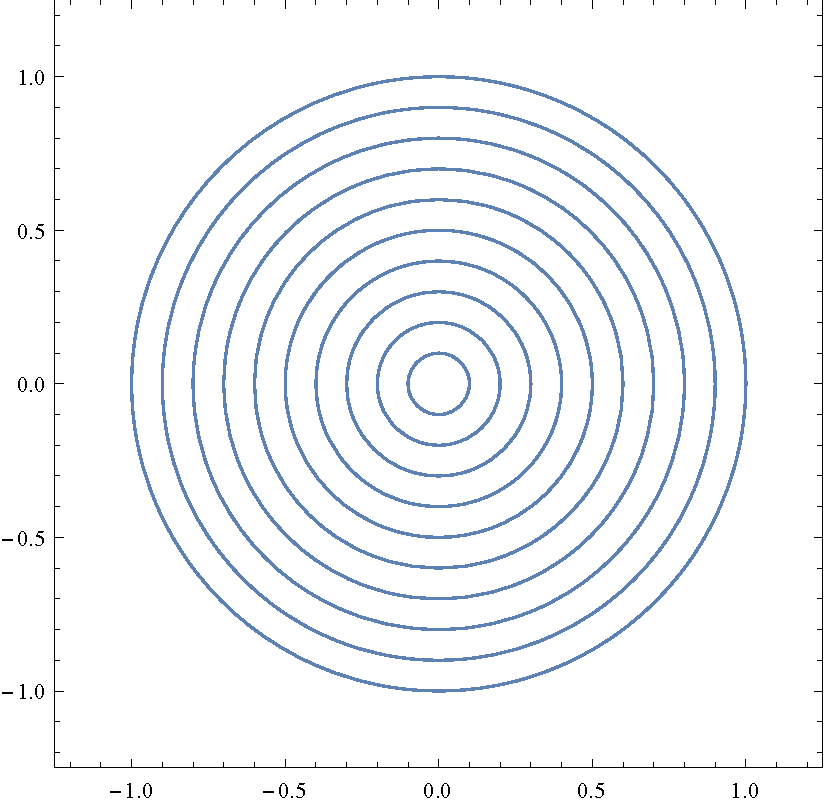
\includegraphics[width = .25\textwidth]{20150513-fig-cone1.pdf}} \quad
\subfigure[$z  = x^2+y^2$]{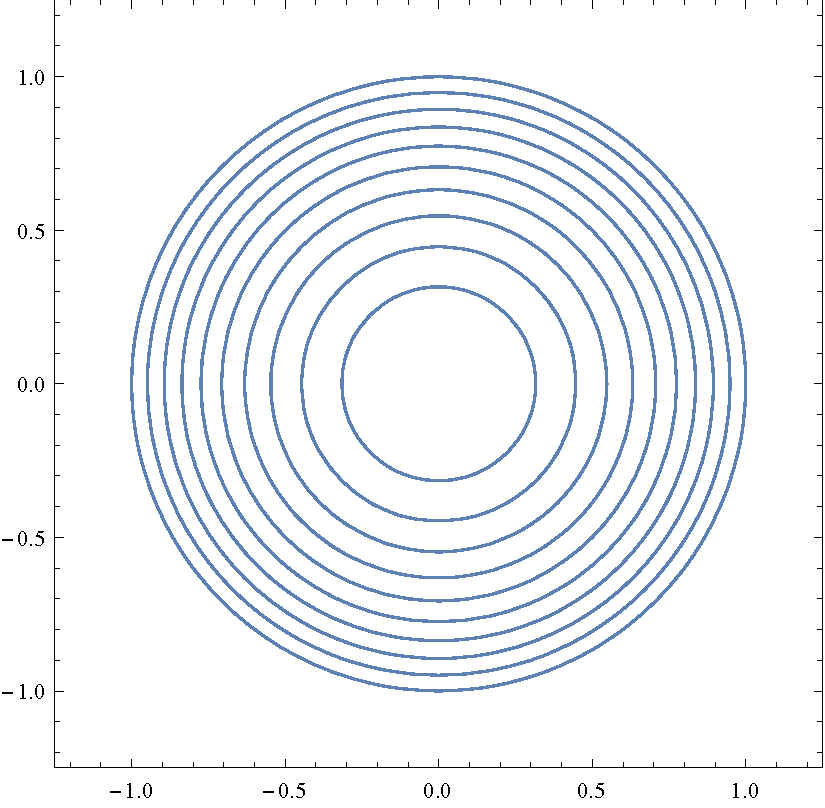
\includegraphics[width = .25\textwidth]{20150513-fig-elliptic-paraboloid1.pdf}}
\end{figure}

この図から明らかに、どちらのグラフも$z$軸回りの回転対称性を持つと分かります。また等高線の密度から、$z = \sqrt{x^2 + y^2}$では高さが一定の間隔で増し、$z = x^2 + y^2$では急激に高さが増していく感じがします。ですがどの程度増えるのかは、この図だけでははっきりしません。詳しい情報を得るためには、他の平面での切断面などが必要です。

\paragraph{$x$軸や$y$軸に垂直な平面での切断}

全く同様に平面$x = c$あるいは$y = c$ ($c\in\mathbb{R}$は定数) を使うことで、それぞれ$x$軸と$y$軸に垂直な平面でグラフを切断できます。

さっきの$z = \sqrt{x^2+y^2}$と$z = x^2 + y^2$で試してみましょう。まずは$x=0$とおくと、式はそれぞれ$z = \sqrt{y^2} = |y|$, $z = y^2$となります。これらが$yz$平面による断面です。そのグラフは次の通りです。

\begin{figure}[h!tbp]
\centering
\subfigure[$z  = |y|$]{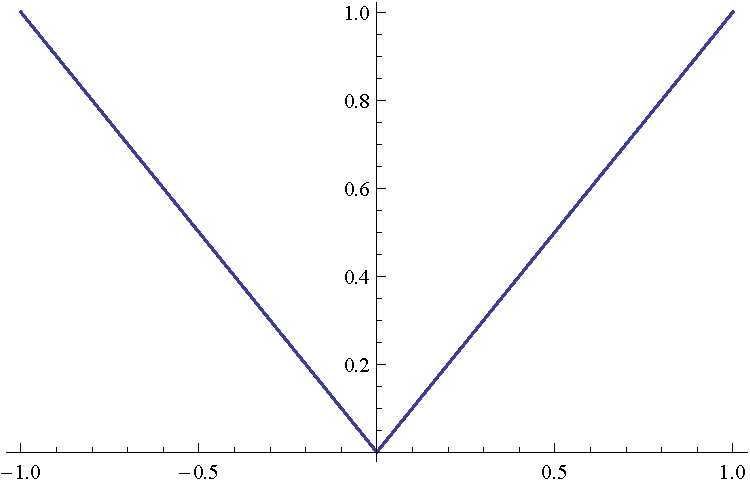
\includegraphics[width = .3\textwidth]{20150513-fig-cone2.pdf}} \quad
\subfigure[$z  = y^2$]{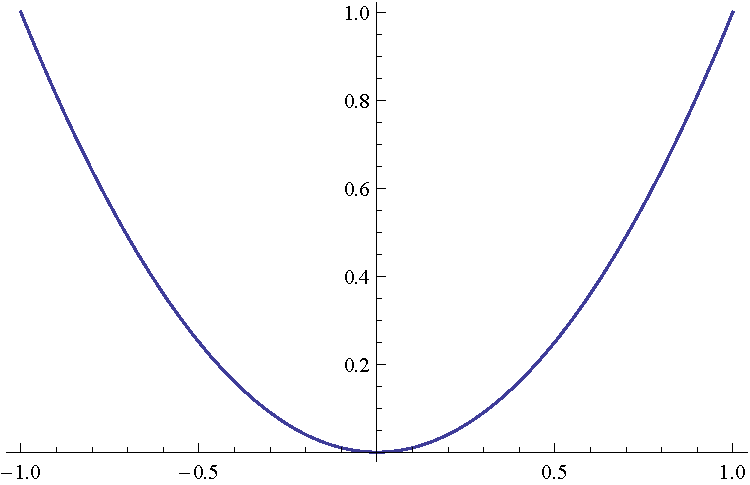
\includegraphics[width = .3\textwidth]{20150513-fig-elliptic-paraboloid2.pdf}}
\end{figure}

あとは$z$軸回りの回転対称性があるので、このグラフを$z$軸回りにぐるっと一周回転させれば求めるグラフの正体が分かります。$z = \sqrt{x^2 + y^2}$は円錐、$z = x^2 + y^2$は回転放物面です。

\begin{figure}[h!tbp]
\centering
\subfigure[$z  = \sqrt{x^2 + y^2}$]{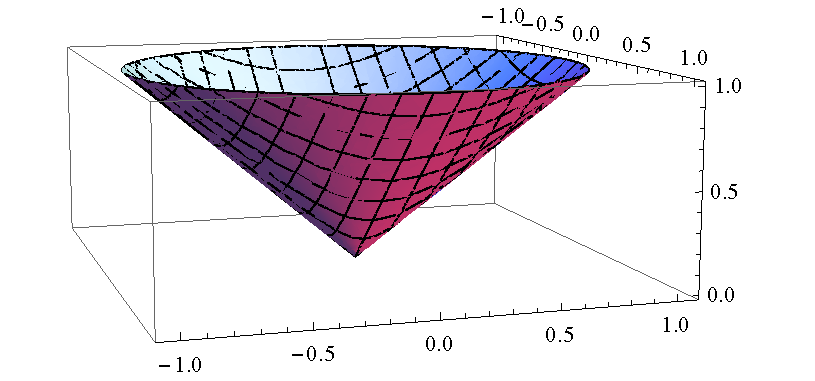
\includegraphics[width = .4\textwidth]{20150513-fig-cone3.pdf}} \quad
\subfigure[$z  = x^2 + y^2$]{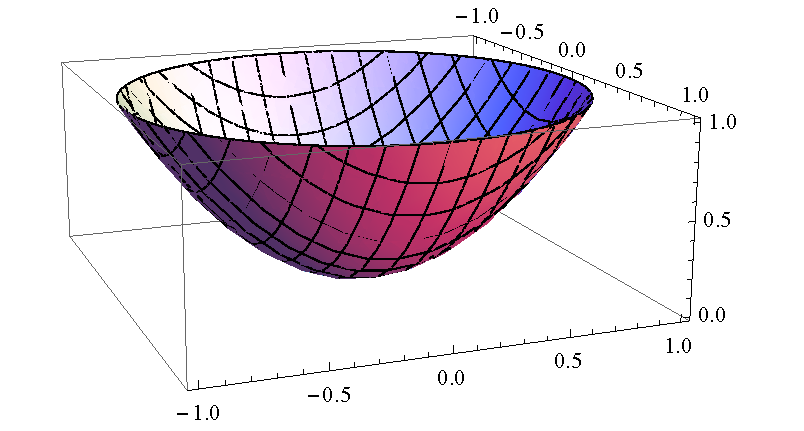
\includegraphics[width = .4\textwidth]{20150513-fig-elliptic-paraboloid3.pdf}}
\end{figure}

また$x$, $y$軸に垂直な平面に関するグラフの切断は、$2$変数函数$f(x, y)$を$x, y$の順に積分するときに役立ちます。特に体積の計算をするときは、まず真っ先にこれらの切断を考えるでしょう。ほとんどの人が大学入試の勉強でやったことがあるはずです。

\subsection{$z$軸を含む平面に関する切断}

続いて平面の方程式のうち、$ax + by = 0$の形のものを考えます。これの法ベクトルは${}^t\!(a, b, 0)$で、$z$軸の方向ベクトル${}^t\!(0, 0, 1)$と直交します。さらに平面$ax + by = 0$は原点を通るので、この平面は$z$軸を含むことが分かりました。したがって方程式$z = f(x, y)$で$ax + by = 0$を連立して$x$ないし$y$を消去すれば、$z$軸を含む平面でどういう形をしているか分かります。この式で$b=0$や$a=0$とした場合は、先ほどの$x$, $y$軸に垂直な平面による切断と一致します。

たとえば方程式$z=xy$のグラフを考えましょう。次のように変形してみます。
\begin{align*}
z = xy = \frac{(x+y)^2 - (x-y)^2}{4}
\end{align*}

この式に$x=y$を代入すると$z=x^2$、$x=-y$を代入すると$-x^2$になります。したがって平面$x=y$での断面は上向きの放物線、それに直交する平面$x=-y$での断面は下向きの放物線となります。ただし、\textbf{この放物線がそのまま$y=\pm x^2$にはならない}ことに気を付けてください。直線$y = x$上で原点からの距離が$1$である点のうち、座標が正のものは$(1/\sqrt{2}, 1/\sqrt{2})$です。ですから$xy$平面の直線$y=\pm x$に$x$軸や$y$軸と同じ目盛りを刻むには、点$(1/\sqrt{2},1/\sqrt{2})$を基準に取らなければいけません。そうすると$(x,y) = (t/\sqrt{2},\pm t/\sqrt{2})$のとき$xy = \pm t^2/2$となりますから、$z = xy$の平面$x = \pm y$による断面の放物線は$y = \pm x^2/2$と合同になります。

一方で等高線は$xy = c$という反比例の式で定まるので、双曲線または$2$直線になります。これを踏まえ、次の平面図を見てください。実線が$z\geq 0$の部分、点線が$z<0$の部分の等高線です。そして斜めの実線と点線がそれぞれ平面$x=y$と$x=-y$に対応し、これらで切断した断面がそれぞれ上向きと下向きの放物線になるわけです。

\begin{figure}[h!tbp]
\centering
\subfigure[$z = xy$を上から見た図]{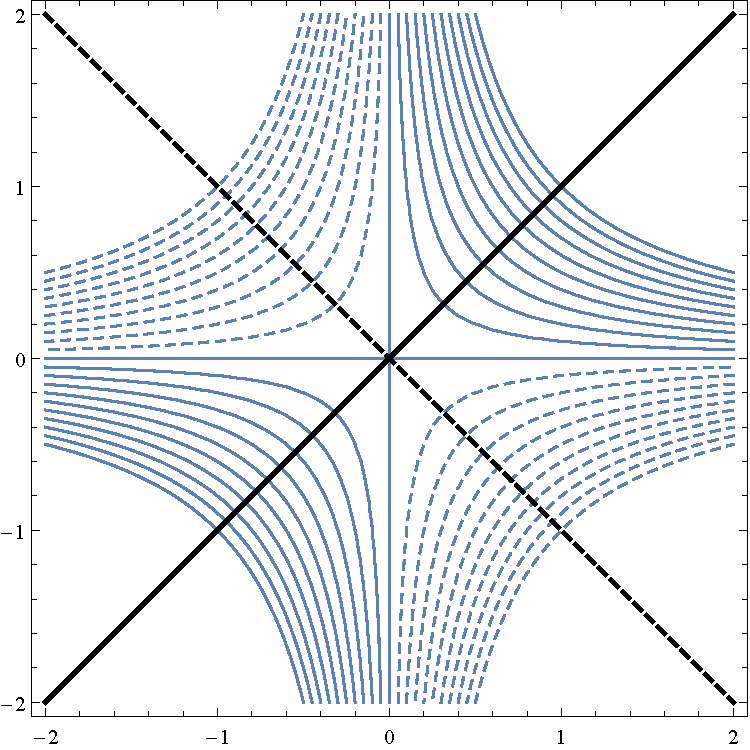
\includegraphics[width = .3\textwidth]{20150513-fig-hyperbolic-paraboloid1.pdf}} \quad
\subfigure[$z = xy$を俯瞰した図]{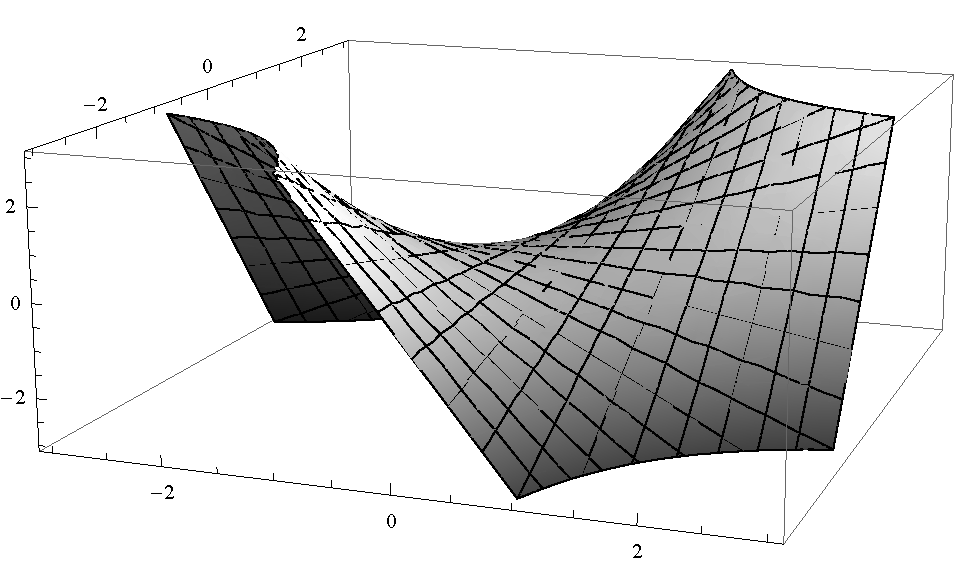
\includegraphics[width = .45\textwidth]{20150513-fig-hyperbolic-paraboloid2.pdf}}
\end{figure}

そして右の図は、曲面$z = xy$を俯瞰した図です。このグラフは双曲放物面と呼ばれます\footnote{テキストに「双曲$2$次形式」とも書いてありますが、これはどちらかというと$x^2-y^2-z=0$という「式の形」を表す言葉です。岩波書店から出ている『数学辞典 第$4$版』を引くと347 Aの項に「双曲放物面」と書いてあるので、その呼び名を使いました。また、このグラフで原点は「接平面が$xy$平面と平行であるが、極大でも極小でもない」という意味で\textbf{鞍点}と呼ばれます。ただしこれは一般名詞であって、グラフを固有名詞的に「馬の鞍」と呼ぶわけではありません。気を付けてください。}。立体的な図を見て等高線が双曲線になること、それから断面に放物線が現れることを納得してください\footnote{PDFファイルの原本 \url{https://github.com/HideakiHosaka/2015_linear_algebra/raw/master/2015linear_algebra.pdf} も必要に応じて見てみてください。カラーな上に拡大可能なので、印刷版より図が綺麗なはずです。}。

\begin{figure}[h!tbp]
\centering
\subfigure[$z = xy$の平面$x = y$による断面]{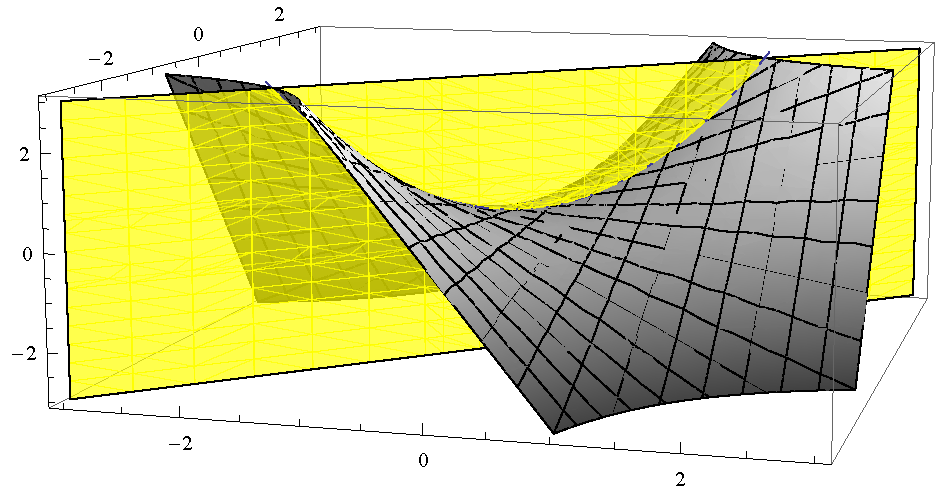
\includegraphics[width = .5\textwidth]{20150513-fig-hyperbolic-paraboloid3.pdf}} \quad
\subfigure[$z = xy$の平面$x = -y$による断面]{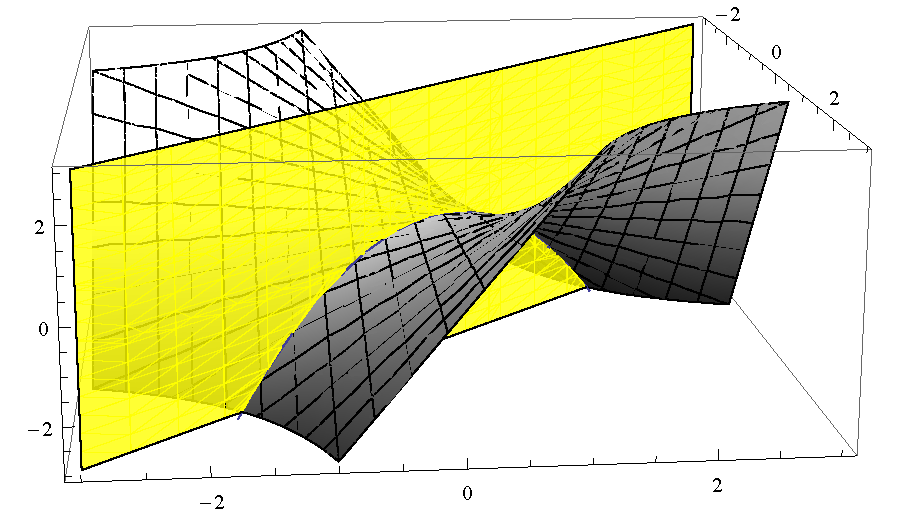
\includegraphics[width = .45\textwidth]{20150513-fig-hyperbolic-paraboloid4.pdf}}
\end{figure}

\section{座標変換とグラフの移動}

$2$変数函数のグラフを理解する別の手段として、グラフの移動を考えます。$1$変数の場合、この手法の最も典型的な例は平方完成です。$2$次函数を平方完成をすると、その$2$次函数が「放物線$y=ax^2$をどうやって動かして作られたか」が分かり、それによってグラフの形状がはっきり分かるのでした。そこで$2$変数函数についても、グラフを動かしましょう。$2$変数の場合は平行移動だけでなく回転移動もできますから、回転移動の方法についても調べます。

また$2$変数以上の函数だと、グラフを移動する以外にも「座標を取り換える」という操作ができます。$1$変数函数だと、せいぜい値域の目盛りを対数軸にして対数プロットをすることがあるくらいで、定義域の目盛りを変えることはありませんでした。ところが$2$変数函数だと、座標の取り換えが極めて有効なケースが出てきます。

\subsection{円柱座標}
平面上の極座標は、$(x,y) = (r\cos\theta, r\sin\theta)$ という式で定義されていました。そこで直交座標$(x,y,z)$のうち$x, y$だけを極座標で置き換えることで$(r,\theta,z)$という座標系が定まります。これを円柱座標といいます\footnote{$3$次元の極座標$(r,\theta,\varphi)$とは別物です。}。

$z=f(x,y)$の式の中にあからさまに$x^2+y^2$が出てくるなどする場合は、円柱座標が役立ちます。たとえばさっきの$z=\sqrt{x^2+y^2}$というグラフを円柱座標で考えてみると、$x^2+y^2=r^2$より$z=\sqrt{r^2}=|r|$となります。だから$z$の値は$\theta$に依存せず、グラフが$z$軸回りの任意の角度に対する回転対称性を持つことが分かります。そして$z$軸を含む平面でグラフを切断すれば、$z=|r|$という絶対値のグラフが現れます。これを回転させることで、元々のグラフは円錐を表していたことが再び分かります。このように$z$軸回りの回転対称性を持つグラフは、円柱座標を使う事ですっきりと理解できます。

$z=x^2+y^2$のグラフでも状況は同じです。こっちでは$z=r^2$となるのでやはり回転対称性を持ち、さらに$z$軸を含む平面での断面は放物線になります。よって放物線を軸に回転させて、元のグラフが回転放物面だと分かります。

\subsection{平行移動}
函数$y=f(x)$のグラフを右に$a$だけ平行移動すると、式は$y=f(x-a)$に変化します。右に$a$ずらすときに$f$の中に$x-a$が入るのでたまに勘違いしそうになりますが、そういうときは$x=0$等で検証してみましょう。平行移動後に$x=0$の位置\textbf{に写ってくる}のは、元々左に$a$だけ移動したところにある$x=-a$の位置の点です。だから平行移動後のグラフで$x=0$における値は$f(-a)$となります。

多変数函数でも全く事情は同じです。$z=f(x,y)$のグラフを$x$軸正の方向に$a$, $y$軸正の方向に$b$だけ平行移動させるとき、平行移動で点$(x, y)$\textbf{に写ってくる}点は$(x-a, y-b)$です。よって平行移動後のグラフは$z=f(x-a,y-b)$になります。

\subsection{回転}

$1$変数のグラフは変数が$x$しかないので、グラフの移動といっても平行移動くらいしかすることがありません。ですが$2$変数のグラフになると、座標の回転ができるようになります。原点中心の回転を調べてみましょう。平行移動のときと同じく、見るべきは「回転移動でどの点がどこに写るか」ではなく「どの点が\textbf{どこから写ってくるか}」です\footnote{後々線型代数の授業で座標変換を考えるときも、これと似たような状況が現れます。}。

複素平面上で原点中心の角度$\theta$回転は、$e^{i\theta}$の掛け算で与えられるのでした。これと$e^{i\theta}e^{-i\theta}(x+iy)=x+iy$より、$\theta$回転で点$(x,y)$\textbf{に写ってくる}点は$e^{-i\theta}(x+iy) = \bigl((\cos\theta) x + (\sin\theta)y \bigr) + i\bigl(-(\sin\theta) x + (\cos\theta) y\bigr)$です。したがって$f(x,y)$を原点中心に$\theta$回転させて得られる函数は、$f(x,y)$の中に今の座標を代入して得られる$f\bigl((\cos\theta) x + (\sin\theta)y, -(\sin\theta) x + (\cos\theta) y\bigr)$です。

% 群の函数への作用

さっきの$z = xy$のグラフは、回転を使うとよく理解できます。$xy$座標系を正の向きに$\pi/4$だけ回転させて$uv$座標系を作ります。すると導いた回転の公式で$\theta=\pi/4$を代入することで、$uv$座標系での点$(u,v)$は$xy$座標系で$\bigl((u+v)/\sqrt{2},(u-v)/\sqrt{2}\bigr)$に化けます。したがって$z = xy$は$uv$座標系で$z = (u^2-v^2)/2$です。こうすれば曲面$z = xy$と$z = x^2-y^2$が回転と縦方向の拡大・縮小で写り合うことが分かります。既に確認した通りですね。ちなみに$z = (u^2-v^2)/2$に直してしまえば、どんな定数$c\in\mathbb{R}$に対しても、平面$u = c$での断面が放物線$z = -v^2 /2$と同じ形だと分かります。実際$z = -v^2/2 + c^2/2$は、放物線$-v^2/2$を上下方向に平行移動したものです。これを$xy$座標系で見れば、平面$y = -x + c$ ($c\in\mathbb{R}$)による断面となります。

また今は$z$軸を中心とする回転を調べましたが、軸が$z$軸と平行である限り、どこであっても回転の計算はできます。既に僕たちはグラフの平行移動の仕方を知っていますから、回転軸が一旦$z$軸と重なるように平行移動し、$z$軸回りの回転をして、さらに最初の平行移動とは逆向きの平行移動をすればOKです。

\section{曲面上の運動と接ベクトル}

\subsection{曲面に沿う曲線と接ベクトル}

$2$変数函数$z=f(x,y)$と平面$\mathbb{R}^2$内の曲線$\gamma$を考えます。各$t\in\mathbb{R}$に対して平面$\mathbb{R}^2$上の点$\gamma(t)\in\mathbb{R}^2$が定まるから、$\gamma(t) = \bigl(x(t), y(t)\bigr)$と書けます。そこで$\gamma(t)$の座標を$z = f(x, y)$に代入する\footnote{写像の言葉で言うなら、曲線を$\gamma\colon\mathbb{R}\rightarrow\mathbb{R}^2$という写像と思い、$2$変数函数$f\colon\mathbb{R}^2\rightarrow\mathbb{R}$の合成$f\circ\gamma$を考えています。}と、$f\bigl(x(t), y(t)\bigr)$は点$\gamma(t)$における$f$の値を表します。こうしてしまえば$f\bigl(x(t), y(t)\bigr)$は$t$の函数ですから、微分することができます。まだ証明していませんが、実は$f\bigl(x(t), y(t)\bigr)$の$t$における微分は$f$と$\gamma'(t) := \bigl(x'(t), y'(t)\bigr)$だけで決まります\footnote{合成函数の微分さえできれば良いのですが、それは多変数の場合「連鎖律」と呼ばれ、少しだけ計算が複雑になります。}。そこで$f\bigl(x(t), y(t)\bigr)$の微分を、$\gamma'(t)$方向の\textbf{方向微分}と言います。$t$を時刻、$\gamma$を点の運動だと思えば、$\gamma'(t)$は時刻$t$における速度ベクトルです。直感的に言うと$f\bigl(\gamma(t)\bigr)$の微分は「$\gamma'(t)$方向に少し動くとどれだけ$f$が変化するか」を表す量ですから、方向微分という言葉がしっくりくるのではないでしょうか。

また$\tilde{\gamma}(t):=\bigl(x(t), y(t), f(x(t), y(t))\bigr)$と置くと、$\tilde{\gamma}(t)$は常に曲面$z = f(x,y)$上の点を表します。したがって$t$を動かすことで、曲面$z = f(x, y)$に沿う曲線が得られます。そこで曲線$\tilde{\gamma}$の座標を$t$で微分すると、$\tilde{\gamma}$の接ベクトルができ、それが曲面$z = f(x, y)$の接ベクトルにもなります。このようにして、曲面の接ベクトルが得られます。

\subsection{偏導函数と接平面}

今の方向微分の話で、特に$\gamma(t) = (a+t, b)$あるいは$\gamma(t) = (a, b+t)$の場合を考えます。つまり$\gamma$は$x$軸や$y$軸の方向を向いた直線の上を、速度$1$で進みます。このとき$f\bigl(\gamma(t)\bigr)$を$t=0$で微分した値を、それぞれ点$(a, b)$における$x$方向、$y$方向の\textbf{偏微分係数}といいます。すなわち
\[
\frac{\partial f}{\partial x}(a, b) := \frac{d}{dt}f(a+t, b)\Bigr|_{t=0}, \quad \frac{\partial f}{\partial y}(a, b) := \frac{d}{dt}f(a, b+t)\Bigr|_{t=0}
\]
です。新しい記号が出てきましたが、計算自体は難しくありません。$x$での偏微分は「$y$を定数と思って、$x$の函数として微分する」というだけです。また$1$変数の場合、微分係数は接線の傾きでした。だから$x$での偏微分係数は、点$(a,b)$における曲面$z = f(x, y)$の$x$軸方向の勾配を表します。

これを知っていると、$2$変数函数のグラフ$z = f(x, y)$の接平面が求められます。$\tilde{\gamma}$の微分が曲面$z = f(x,y)$の接ベクトルでした。その式に$x$方向の偏微分と$y$方向の偏微分を代入すると
\[
\biggl(1, 0, \frac{\partial f}{\partial x}(a, b)\biggr),\quad \biggl(0, 1, \frac{\partial f}{\partial y}(a, b)\biggr)
\]
が曲面$z = f(x,y)$の点$(a, b)$における接ベクトルだと分かります。これらのベクトルは$1$次独立ですから、点$(a, b)$における接平面はこれら$2$本のベクトルによって張られます。したがって外積を使って、接平面の法ベクトルが
\[
\biggl(\frac{\partial f}{\partial x}(a, b), \frac{\partial f}{\partial y}(a, b), -1\biggr)
\]
と分かります。これで接平面の方程式における$x, y, z$の係数が決まりました。あとは接平面が点$\bigl(a, b, f(a,b)\bigr)$を通るよう調整すれば、接平面の方程式
\[
\frac{\partial f}{\partial x}(a, b) (x-a) + \frac{\partial f}{\partial y}(a, b) (y-b) - \bigl( z - f(a,b)\bigr) = 0
\]
が求まります。

\section{解答など}

\subsection{穴埋め問題の解答}

既に一通りの問題を解説していますが、穴埋め問題の解答だけをもう一度まとめておきます。

\begin{tabular}{c@{\hspace{0.1zw}}l@{\hspace{1zw}}c@{\hspace{0.1zw}}l@{\hspace{1zw}}c@{\hspace{0.1zw}}l@{\hspace{1zw}}c@{\hspace{0.1zw}}l@{\hspace{1zw}}c@{\hspace{0.1zw}}l@{\hspace{1zw}}c@{\hspace{0.1zw}}l@{\hspace{1zw}}c@{\hspace{0.1zw}}l@{\hspace{1zw}}c@{\hspace{0.1zw}}l@{\hspace{1zw}}}
(1) & 平面 & (2) & 双曲放物面 & (3) & $z$軸 & (4) & 回転対称性 & (5) & 円錐 & (6) & 回転放物面 & (7) & $a$ & (8) & $b$ \\
(9) & $\sqrt{c}$ & (10) & $2xy$ & (11) & 双曲放物面 & (12) & 双曲線 & (13) & $a$ & (14) & $b$ & (15) & $1/2$ & (16) & $-1/2$ \\
\end{tabular}

\subsection{グラフ}
$z = xy$のグラフは既に描きました。$z = x \sin y$と$z = \sin x\sin y$のグラフは次の通りです。グラフの雰囲気が分かるよう、問題より少し範囲を広げて描画しています。
\begin{figure}[h!tbp]
\centering
\subfigure[$z  = x \sin y$]{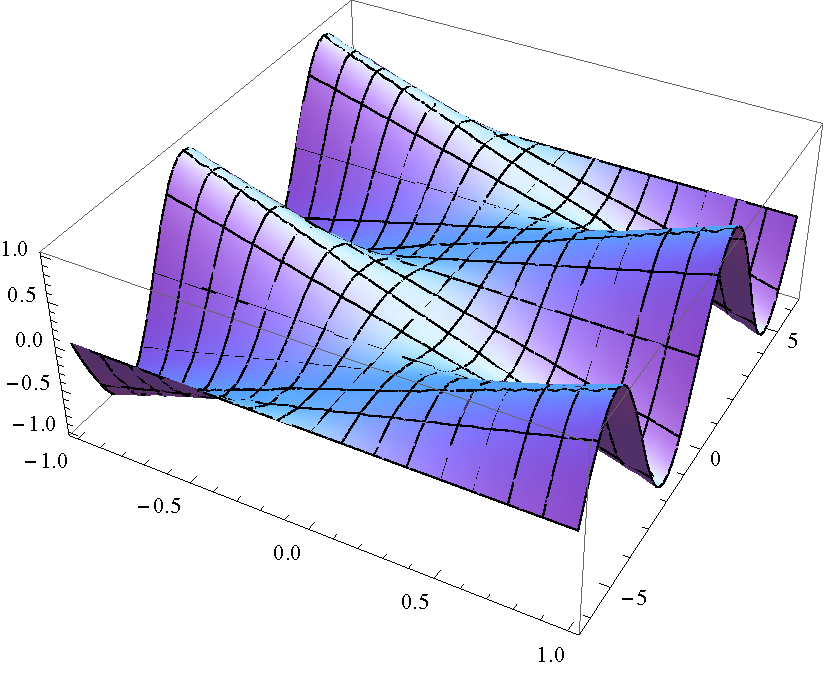
\includegraphics[width = .4\textwidth]{20150513-fig-problem-b.pdf}} \quad
\subfigure[$z  = \sin x \sin y$]{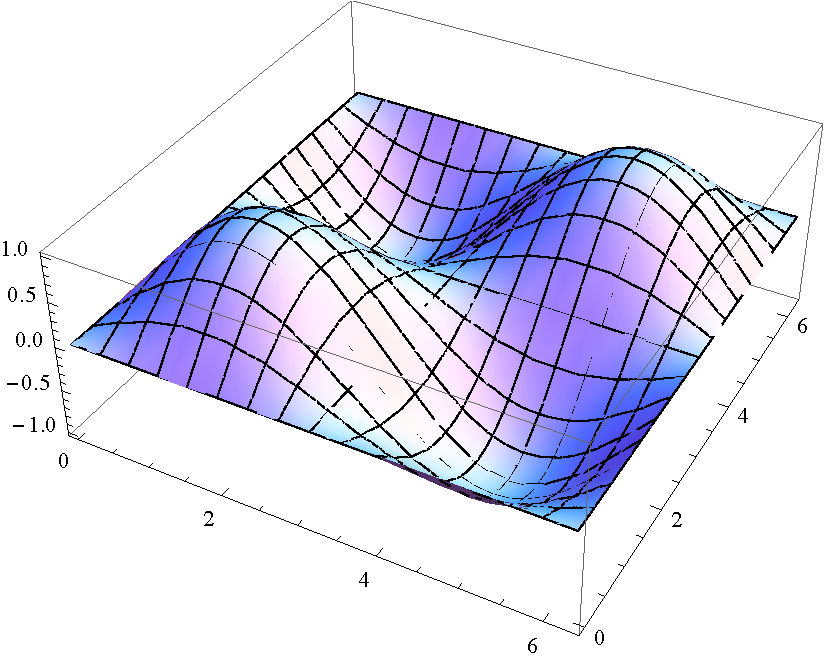
\includegraphics[width = .4\textwidth]{20150513-fig-problem-c.pdf}} \quad
\end{figure}

ちなみに、これらのグラフはMathematicaを使って描いています。Mathematicaの使い方については、たとえば「はいぱーワークブック」の29章\footnote{\url{http://hwb.ecc.u-tokyo.ac.jp/current/applications/mathematica/}}や、そこに紹介されている参考文献などを読んでください。


\chapter{行列とその演算}

\lectureinfo{2015年5月20日 1限}

今回のテーマは行列の計算です。行列の計算を理解できていない人はいないようでしたが、\textbf{計算ミスをする人が少なくありませんでした}。行列の計算は今後多用しますから、この機会に十分慣れておいてください。

\section[総和記号Σの使い方]{総和記号$\sum$の使い方} \label{section:usage_of_sum_symbol}\index{sigma@$\sum$ (総和記号)}

行列の積の計算やこの後でやる行列式の計算では、とにかく$\sum$記号が式中にたくさん現れます。そこで最初に、$\sum$の色々な使い方をまとめておきましょう。必要に応じて読んでください。

\subsection{最もありふれた使い方}

総和記号$\sum$の使い方として、最もありふれたものは
\[
\sum_{i = 1}^n a_i := a_1 + a_2  + \cdots + a_n
\]
というものでしょう。$n$個の数$a_1,a_2,\ldots,a_n$が与えられたとき、それの全ての和を上に書いたように、$\sum$記号で表すのでした。$\sum$記号は数学でよく現れる「数列の和」を表せるという意味で便利な記号ですが、それ以上に「記号操作で複雑な計算を片付けられる」という点が強力です。そのことを、以下で見ていきましょう。

\paragraph{線型性}
$\sum$の最も大事な性質は、次の\textbf{線型性}です。
\begin{align*}
\sum_{k = 1}^n  (a_k + b_k) &= \sum_{k = 1}^n a_k + \sum_{k = 1}^n b_k, \qquad
\sum_{k = 1}^n \alpha a_k = \alpha \sum_{k = 1}^n a_k
\end{align*}
式自体の意味は単純で、$1$つ目は足し算の順序の入れ替え、$2$つ目はかっこでくくる操作を表しています。
\begin{align*}
(a_1 + b_1) + (a_2 + b_2) + \cdots + (a_n + b_n) &= (a_1 + a_ 2 + \cdots + a_n) + (b_1 + b_2 + \cdots + b_n) \\
\alpha a_1 + \alpha a_2 + \cdots + \alpha a_n &= \alpha (a_1 + a_2 + \cdots + a_n)
\end{align*}
実際に式変形をするときは、線型性の公式を左から右、右から左の両方で使います。すなわち今の式を
\begin{itemize}
\item 変数が同じ範囲を走る$\sum$が足されているときは、それをひとまとめにしてよい
\item $\sum$の中に足し算があれば、それを$2$つの$\sum$に分割できる
\item $\sum$の変数と関係ない数は、いつでも$\sum$を前後に飛び越えられる
\end{itemize}
と読むわけです。

\paragraph{変数のシフトと和の順序の反転}

$\sum$の変数は、ずらすことが可能です。たとえば
\[
\sum_{k = 1}^n a_k = a_1 + a_2 + \cdots + a_n, \qquad \sum_{k = 0}^n a_{k+1} = a_1 + a_2 + \cdots + a_n
\]
ですね。項を書き出してしまえば当たり前ですが、$k$が走る範囲をずらしても、それに合わせて$\sum$の中の式に出てくる$k$を適当にずらせば、表す式は全く同じになります。

同じようにして、足す順序を逆順にすることもできます。$a_1 + a_2 + \cdots + a_n = a_n + a_{n-1} + \cdots + a_1$ですから
\[
\sum_{k = 1}^n a_k = \sum_{k = 1}^n a_{n+1-k}
\]
という式が成り立ちます。

これらの変数の変換は、主に線型性と組み合わせて$2$つの$\sum$をくっつけるときに使います。たとえば$\sum_{k = 1}^n k$の公式は、次のようにして導くことができます。
\begin{align*}
2 \sum_{k = 1}^n k
&= \sum_{k = 1}^n k + \sum_{k = 1}^n k
= \sum_{k = 1}^n k + \sum_{k = 1 }^n (n + 1 - k)
= \sum_{k = 1}^n \bigl\{ k + (n + 1 - k) \bigr\}
= \sum_{k = 1}^n (n+1) 
= n(n+1)
\end{align*}
もう一つ別の証明を挙げておきます。こっちの手法は、$\sum k^2$や$\sum k^3$の公式を導くのにも使えます。
\begin{align*}
(n+1)^2 -1
&=\sum_{k = 1}^n \{(k + 1)^2 - k^2\}
= \sum_{k = 1} ^n (2k+1) 
= 2\sum_{k = 1}^n k + \sum_{k = 1}^n 1
= 2\sum_{k = 1}^n k + n \\
\therefore \sum_{k = 1} ^n  k
&= \frac{(n+1)^2-1-n}{2}
= \frac{n^2 + n}{2}
\end{align*}

どちらの証明でも、$1$つ$1$つの式変形が「和の順序の反転」や「線型性で$\sum$をまとめる / ばらす」といった操作だけしか行っていないことに気を付けてください。このように「$\sum$の公式をそのまま当てはめる」という操作を繰り返すだけで証明を完了できることが、$\sum$を使う大きなメリットなのです。

% 差分の話

%\paragraph{公式}
%\[
%\sum_{i = 1}^n i = \frac{n(n+1)}{2}, \sum_{i = 1}^n r^i = \frac{r^{n+1} - 1}{r - 1}
%\]

\subsection{集合を走る変数に関する和}

さて$\sum_{k =1}^n a_k$は「$k$を順番に$1,2,\ldots,n$と動かし、出てくる項を全部足す」という意味でした。ですが「順番に足す」という意味は別に大事ではありません\footnote{ただし、たまに$n = 0$のとき「$\sum_{k = 1}^n a_k = 0$」という式が出ます。このような場合は$\sum$を$1$から「順に足す」という意味で捉えないと、式を正しく解釈できません。}。どうせ足し算だから、順序を入れ替えたって結果は変わらない\footnote{ここで考えているのは有限個の足し算だけです。無限級数などの代数的に扱えない場合は、全く考えていません。}からです。そこで順番を考えず、「集合のそれぞれの元に対応する項を足す」という意味でも$\sum$を使います。たとえば
\[
\sum_{k\in\{1,3,5\}} a_k = a_1 + a_3 + a_5
\]
という感じです。$\{1,3,5\}$の元は$1$と$3$と$5$だから、$k$が$1,3,5$を動くのに合わせて対応する$a_k$、つまり$a_1$と$a_3$と$a_5$を足し合わせるというのが左辺の$\sum$の意味です。新しい$\sum$を使えば、これまで使っていた$\sum$は
\[
\sum_{k = 1}^n a_k = \sum_{k\in\{1,2,\ldots,n\}} a_k
\]
と書き表せます。だから新しい$\sum$の使い方は、今までの$\sum$が拡張されたものになっています。後々見ていくように、$\sum$の変数に整数以外のものを使えるのは、実は非常に役立ちます。

さらに省略した書き方として、$\sum$の下に「変数の満たすべき条件」を書く場合があります。たとえば
\[
\sum_{\substack{1\leq k\leq 5\\ \text{$k$は奇数}}} a_k = a_1 + a_3 + a_5
\]
と書きます。集合$\{k\in\mathbb{N}\mid 1\leq k\leq 5, \text{$k$は奇数}\}$は$\{1,3,5\}$と同じです。この集合を$\sum$の下の狭いスペースに書くと非常に見苦しいので「縦棒の右側に書かれる条件だけを$\sum$の下に書いてしまおう」という魂胆です。だから
\[
\sum_{1\leq k\leq 5} a_k = \sum_{k\in\{1,2,3,4,5\}} a_k = \sum_{k = 1}^5 a_k = a_1 + a_2 + a_3 + a_4 + a_5
\]
などという意味になります。このとき一番左の表記法では``$k\in\mathbb{N}$''という条件が地味に抜け落ちますが、その部分については「読者が空気を読んで察する」という暗黙のルールがあります\footnote{勉強する人に向かって「空気読め」は割とヒドい言葉のような気がするのですが、ちょっとでも新しい$\sum$記号を使ってみると、逆に「一々$\sum$の下に集合を書くなんてかったるい」と思うようになってしまうんですよね……。}。頑張って読み解いてください。

さらに、この$\sum$記法に慣れるとこんなこともできます。
\[
\sum_{k \in A\cup B} a_k = \sum_{k \in A} a_k  + \sum_{k \in B} a_k - \sum_{k \in A\cap B} a_k
\]
$\sum$の変数が集合を走る場合、集合の分割に応じて$\sum$を分割できます。もし和にダブりがあればその部分を引いて補正しなければいけませんが、ダブりなくばらせば第$3$項は消えます。このような$\sum$の分割は、$\sum$を部分的に計算する場合に役立ちます。

\subsection{変数について}

ここで、$\sum$の変数について$2$つほど注意をしておきます。

\paragraph{ダミー変数}

次の式を見てください。
\[
\sum_{k = 1}^n a_k = \sum_{l = 1}^n a_l
\]
当たり前の式ですが、ここで大事なのは\textbf{$\sum$で走る文字は自由に取り換えても良い}という点です。左辺の$\sum$では、$k$は「$1$から$n$までの整数を動くこと」だけを示すのに使われているのであって、$k$という文字自体が式全体で意味を持っているわけではありません。$k$という文字は、$\sum$の中だけで有効です。こういう変数を\textbf{ダミー変数}\index{だみーへんすう@ダミー変数}と言います。

$\sum$を$1$個単独で使ってる場合は、ダミー変数の文字を変えるご利益はそんなにありません。せいぜい複素数を足し算する時、虚数単位とこんがらがらないよう変数を$i$から$j$に変えるくらいでしょうか。ですが$\sum$が入った複数個の式をかけて変形するようになると、割と頻繁に変数の衝突が起きたりします。そういう場合に文字の取り換えは、地味ですが計算を遂行するのに大変役立ちます。

\paragraph{変数のスコープ}

今のダミー変数について、$\sum$の変数は\textbf{式中の一部分でのみ意味がある}と言いました。この変数が有効な範囲を、プログラミングの言葉で\textbf{変数のスコープ}\index{へんすうのすこーぷ@変数のスコープ}といいます。たとえば
\[
\sum_{k=1}^n \uwave{(2k - 1)} = n^2
\]
の左辺における$k$のスコープは、下線を引いた$2k-1$の場所です。

当たり前のことですが、$\sum$で使われる変数はスコープ外で意味を持ちません。ですから式を見直してみて「$\sum$の外にダミー変数が飛び出していた」とか「$\sum$の計算をし終わった後にダミー変数が残っていた」などという場合、スコープを考えるだけで明らかに計算ミスがあると分かります。今みたいな単純な式だと気になりませんが、$\sum$の入った複雑な式では変数のスコープを意識すると計算がしやすくなります。心の片隅に置いといてください。

\subsection{二重和} \index{にじゅうわ@二重和}

ここまで$\sum$の使い方を色々説明してきましたが、実用面を考えると、さらに一歩踏み込んで多重の$\sum$を取り扱う必要があります。

計算の定義自体は今までの$\sum$と変わりません。たとえば
\[
\sum_{k = 1}^m \sum_{l  = 1}^n a_{k,l} = \sum_{k = 1}^m \Biggl\{\sum_{l  = 1}^n a_{k,l}\Biggr\}
\]
というように「内側の$\sum$をまず足し、その結果を外側の$\sum$でさらに足し合わせる」というだけです。$\sum$を元々「$1$列に並べた数を足し合わせる」という方法で使っていたことになぞらえれば、二重和は「長方形に並べた数を足し合わせる」という感じです。ただ二重和の場合
\[
\sum_{k = 1}^m \sum_{l  = 1}^k a_{k,l} = \sum_{k = 1}^m \Biggl\{\sum_{l  = 1}^k a_{k, l}\Biggr\} = (a_{1, 1}) + (a_{2, 1} + a_{2, 2}) + (a_{3, 1} + a_{3, 2} + a_{3, 3}) + \cdots
\]
のように、「外側の$\sum$のダミー変数を使って、内側の$\sum$における変数の範囲を指定する」という技ができたりします。上の例では、三角形に並べた数を全部足すという意味になります。

このような場合に、足し算の順序を上手くコントロールするための変数の扱い方を見ていきましょう。

\paragraph{和の順序の交換}\index{じゅんじょこうかん@($\sum$の) 順序交換} 一番基本的な二重和
\begin{align*}
\sum_{k = 1}^m \sum_{l  = 1}^n a_{k, l} 
= \sum_{k = 1}^m (a_{k, 1} + a_{k, 2} + \cdots + a_{k, n} )
=
\begin{array}{c@{\,}c@{\,}c@{\,}c@{\,}c@{\,}c}
 &a_{1, 1}  &+ &a_{1, 2} &+ \cdots + &a_{1, n} \\
+ &a_{2, 1} &+ &a_{2, 2} &+ \cdots + &a_{2, n} \\
+ & \cdots &\cdots \\
+ &a_{m, 1} &+ &a_{m, 2} &+ \cdots + &a_{m, n}
\end{array}
\end{align*}
を考えてみましょう。この計算は、各行を横向きに足し合わせた結果を縦に足し合わせても、各列を縦向きに足し合わせた結果を横に足し合わせても全く同じ結果になります。これを$\sum$で表現すると
\[
\sum_{k = 1}^m \sum_{l  = 1}^n a_{k, l} =
\sum_{l  = 1}^n \sum_{k = 1}^m a_{k, l} 
\]
となります。一方、
\begin{align*}
\sum_{k = 1}^n \sum_{l  = 1}^k a_{k,l}
= \sum_{k = 1}^n (a_{k, 1} + a_{k, 2} + \cdots + a_{k, k})
=
\begin{array}{c@{\,}c@{\,}c@{\,}c@{\,}c}
 &a_{1, 1} \\
+ &a_{2, 1} &+& a_{2, 2} \\
+ &\cdots \\
+ &a_{n, 1} &+& a_{n, 2} &+ \cdots + a_{n, n}
\end{array}
\end{align*}
のような場合、外側と内側の$\sum$を安直に入れ替えることはできません。この事実は「内側の$\sum$の上限を与える$k$が、外側の$\sum$のスコープの外に出られない」とも言えます。ですから「内側の$\sum$の範囲指定に外側の$\sum$の変数が使われていない限り、$2$つの$\sum$の順番を入れ替えることができる」というのが結論です。$\sum$の変数が集合を走る場合でも、同じことが言えます。

\paragraph{$\sum$の結合と分割} 次の式を見てください。
\[
\sum_{k = 1}^m \sum_{l = 1}^n a_{k, l} = \sum_{1\leq k\leq m} \sum_{1\leq l\leq n} a_{k, l} = \sum_{\substack	{1\leq k \leq m\\ 1\leq l\leq n}} a_{k, l}
\]
こんな感じで、$2$つの$\sum$をくっつけることができます。元々の二重和を「$k$が$\{1,2,\ldots,m\}$を走り、$l$が$\{1,2,\ldots,n\}$を走る」と書き換えた上で、さらに集合の直積を利用して「$(k,l)$が$\{1,2,\ldots,m\}\times\{1,2,\ldots,n\}$を走る」と書き換えました。こういう風に集合の直積を使うと、$2$つの$\sum$を$1$つにくっつけられます。逆に$\sum$の変数が直積集合を走るときは、$\sum$を$2$つにばらすことができます。

あんまり大した意味が無いようにも見えますが、三重以上に$\sum$が重なる状況では、$\sum$を$1$つにまとめると案外式が見やすくなったりします。また「$\sum$の変数は集合の上を走る」という意識を持っておくと、$\sum$の変数を操作するときに、式が正しいかどうかを変数の走る集合が等しいかどうかという問題に帰着させて考えられます。

\paragraph{変数変換} 最後に、$\sum$の変数変換を紹介します。次の二重和を見てください。
\begin{align*}
\sum_{k = 1}^n \sum_{l  = 1}^k a_{k,l}
=
\begin{array}{c@{\,}c@{\,}c@{\,}c@{\,}c}
 &a_{1, 1} \\
+ &a_{2, 1} &+& a_{2, 2} \\
+ &\cdots \\
+ &a_{n, 1} &+& a_{n, 2} &+ \cdots + a_{n, n}
\end{array}
\end{align*}
この足し方を図示したのが、次の一番左の図です。内側の$\sum$で足される項を、矢印で繋いでいます。
\begin{figure}[h!tbp]
\centering
\begin{picture}(80,90)
\put(0,0){\vector(0,1){80}}
\put(0,0){\vector(1,0){80}}
\put(82,-3){$k$}
\put(5,75){$l$}
\put(10,10){\circle*{3}}
\put(30,10){\circle*{3}}
\put(30,10){\vector(0,1){18}}
\put(30,30){\circle*{3}}
\put(50,10){\circle*{3}}
\put(50,10){\vector(0,1){18}}
\put(50,30){\circle*{3}}
\put(50,30){\vector(0,1){18}}
\put(50,50){\circle*{3}}
\put(70,10){\circle*{3}}
\put(70,10){\vector(0,1){18}}
\put(70,30){\circle*{3}}
\put(70,30){\vector(0,1){18}}
\put(70,50){\circle*{3}}
\put(70,50){\vector(0,1){18}}
\put(70,70){\circle*{3}}
\end{picture}\qquad\qquad
\begin{picture}(80,90)
\put(0,0){\vector(0,1){80}}
\put(0,0){\vector(1,0){80}}
\put(82,-3){$k$}
\put(5,75){$l$}
\put(10,10){\circle*{3}}
\put(10,10){\vector(1,0){18}}
\put(30,10){\circle*{3}}
\put(30,10){\vector(1,0){18}}
\put(30,30){\circle*{3}}
\put(30,30){\vector(1,0){18}}
\put(50,10){\circle*{3}}
\put(50,10){\vector(1,0){18}}
\put(50,30){\circle*{3}}
\put(50,30){\vector(1,0){18}}
\put(50,50){\circle*{3}}
\put(50,50){\vector(1,0){18}}
\put(70,10){\circle*{3}}
\put(70,30){\circle*{3}}
\put(70,50){\circle*{3}}
\put(70,70){\circle*{3}}
\end{picture}\qquad\qquad
\begin{picture}(80,90)
\put(82,-3){$k$}
\put(5,75){$l$}
\put(0,0){\vector(0,1){80}}
\put(0,0){\vector(1,0){80}}
\put(10,10){\circle*{3}}
\put(10,10){\vector(1,1){18}}
\put(30,10){\circle*{3}}
\put(30,10){\vector(1,1){18}}
\put(30,30){\circle*{3}}
\put(30,30){\vector(1,1){18}}
\put(50,10){\circle*{3}}
\put(50,10){\vector(1,1){18}}
\put(50,30){\circle*{3}}
\put(50,30){\vector(1,1){18}}
\put(50,50){\circle*{3}}
\put(50,50){\vector(1,1){18}}
\put(70,10){\circle*{3}}
\put(70,30){\circle*{3}}
\put(70,50){\circle*{3}}
\put(70,70){\circle*{3}}
\end{picture}
\end{figure}

そして図中にも描いたように、この二重和は色々な足し方ができます。この図をじっくり見れば
\[
\sum_{k = 1}^n \sum_{l = 1}^k a_{k, l}
= \sum_{l = 1}^n \sum_{k = l}^n a_{k, l}
= \sum_{p = 1}^n \sum_{k = 1}^{n + 1 - p} a_{p - 1 + k, k}
\]
が分かるはずです。集合で言えば、$\{(k,l)\in\{1,2,\ldots,n\} \mid l \leq k\}$を鉛直な直線や、あるいは軸と$45^{\circ}$の傾きをなす直線でスライスして分割しているわけです。このように二重和では「格子の各点に項が対応している」と捉えることで、外と中の$\sum$をそのまま入れ替えることはできなくても、足し方を色々変えることができます。特に、斜めの足し算はしばしば式変形のキーポイントになります。

$\sum$の変数変換は実際にやってみると案外間違えやすいのですが、そういう時はきちんと格子を描き「どの範囲の項が足されるか」を絵で表しましょう。そうすればぐっと間違いは減るはずです。

\subsection{総積記号}\index{pi@$\prod$ (総積記号)}
ちなみに$\sum$の掛け算バージョンもあって、それは$\prod$ (パイ) という記号で表されます。使い方は$\sum$と全く同じで
\[
\prod_{k = 1}^n a_i = a_1 a_2 \cdots a_k
\]
という意味です。たとえば$\prod_{k = 1}^n k = n!$など。$\sum$のときと同様、変数は集合を走ることもあります。

この記号も色々使いどころがあります。特に
\[
\sum_{k = 1}^n \log a_k = \log \prod_{k = 1}^n a_k, \qquad \prod_{k = 1}^n p^{a_k} = p^{\sum_{k = 1}^n a_k}
\]
という形の式変形は知っておくと、計算がサクサク進むと思います。

\section{行列とその演算}

数を縦に$m$個、横に$n$個並べたものを$m\times n$型あるいは$(m, n)$型の\textbf{行列}\index{ぎょうれつ@行列}といいます。また、行列の中にある一つ一つの数を\textbf{成分}といいます。特に$i$行$j$列\footnote{横の並びが行 (row), 縦の並びが列 (column) です。自動車レースのフロント・ローとか、化学で使うカラムクロマトグラフィーといった言葉を思い出すと「rowが横、columnが縦」を間違えにくくなるかもしれません。}にある成分を指して$(i,j)$成分という呼び方をします。成分を表すときは
\begin{itemize}
\item $A_{ij}$のように右下に$ij$をつけることで、行列$A$の$(i, j)$成分を表す
\item $(i, j)$成分が$a_{ij}$である行列のことを、$(a_{ij})_{\substack{1\leq i\leq m\\ 1\leq n\leq n}}$と表す
\end{itemize}
といった記法も使います。覚えておきましょう。

行列は数学の色々なところで使います。たとえば連立$1$次方程式を解いたり、微分方程式を解いたりといった用途に使えますし、また他の分野への応用もたくさんあります。じっくり勉強して、行列の扱いに慣れていってください。

\subsection{行列の和と積}

行列に対しては和\index{わ@(行列の) 和}と積\index{せき@(行列の) 積}が定義されます。まずはその定義を確認します。同じ型の行列に対しては「同じ位置にある成分を足す」、すなわち
\[
\begin{pmatrix}
a_{11} & a_{12} & \cdots & a_{1n} \\
a_{21} & a_{22} & \cdots & a_{2n} \\
\vdots & \vdots & \ddots & \vdots \\
a_{m1} & a_{m2} & \cdots & a_{mn}
\end{pmatrix}
+
\begin{pmatrix}
b_{11} & b_{12} & \cdots & b_{1n} \\
b_{21} & b_{22} & \cdots & b_{2n} \\
\vdots & \vdots & \ddots & \vdots \\
b_{m1} & b_{m2} & \cdots & b_{mn}
\end{pmatrix}
=
\begin{pmatrix}
a_{11} + b_{11} & a_{12} + b_{12} & \cdots & a_{1n} + b_{1n} \\
a_{21} + b_{21} & a_{22} + b_{22} & \cdots & a_{2n} + b_{2n} \\
\vdots & \vdots & \ddots & \vdots \\
a_{m1} + b_{m1} & a_{m2} + b_{m2} & \cdots & a_{mn} + b_{mn}
\end{pmatrix}
\]
と定めます。そして積は、$(m,n)$型行列$A$と$(n,l)$型行列$B$との間でだけ定義され、その$(i,j)$成分は
\[
(AB)_{ij} = \sum_{k = 1}^n a_{ik}b_{kj}
\]
です。これだと何をやっているか分からないのですが、行列を
\[
\biggl(
\begin{array}{ccc}
a_{11} & a_{12} & a_{13} \\ \hline
a_{21} & a_{22} & a_{23} 
\end{array}
\biggr)
\Biggl(
\begin{array}{c|c|c}
b_{11} & b_{12} & b_{13} \\
b_{21} & b_{22} & b_{23} \\
b_{31} & b_{32} & b_{33}
\end{array}
\Biggr)
\]
と区切れば、$AB$の$(i,j)$成分は「$A$の$i$行目と$B$の$j$列目との内積」だと分かります。慣れないうちは、こうやってきちんと行と列を区切ることをお勧めします。

こんなややこしい定義をするのには相応の事情があるのですが、そんなことよりも\textbf{行列の積は役立つ}という事実が大事です。数学で使うだけでなく、Googleが検索クエリを処理するとき\footnote{学習院大学の田崎晴明先生が執筆中の教科書 \url{http://www.gakushuin.ac.jp/~881791/mathbook/index.html} 内の「グーグルのページランク」の節に、解説があります。あるいは原論文 \url{http://infolab.stanford.edu/pub/papers/google.pdf} を見ても良いでしょう。}とか、生物の記憶のシミュレーションをするときとか\footnote{たとえば池谷裕二『進化しすぎた脳』(講談社ブルーバックス) の付録を参照。}、その他行列の使い道は山ほどあります。理論的な場面でも使うので、計算をコンピュータに丸投げできず、人間が手計算をしなければいけない場面もしばしばあります。ですので行列の掛け算の仕方は徹底的に練習して、体で覚えてください。

\subsection{行列の積の性質}
行列の積で非常に特徴的なのは\textbf{順序を変えると結果が変わる}という性質です。具体例を一つやってみます。

\paragraph{問8の解答$+\alpha$}
\begin{align*}
\biggl(
\begin{array}{ccc}
1 & 2 & 4 \\ \hline
3 & 1 & 1
\end{array}
\biggr)
\Biggl(
\begin{array}{c|c}
-2 & 2 \\
7 & 5 \\
-1 & -3
\end{array}
\Biggr)
=
\begin{pmatrix}
8 & 0 \\
0 & 8
\end{pmatrix}, 
\Biggl(
\begin{array}{cc}
-2 & 2 \\ \hline
7 & 5 \\ \hline
-1 & -3
\end{array}
\Biggr)
\biggl(
\begin{array}{c|c|c}
1 & 2 & 4 \\
3 & 1 & 1
\end{array}
\biggr)
=
\begin{pmatrix}
4 & -2 & -6 \\
22 & 19 & 33 \\
-10 & -5 & -7
\end{pmatrix}
\end{align*}

\paragraph{非可換性}\index{ひかかんせい@非可換性}

今の例では、行列の積$AB$と$BA$の結果がサイズ違いになりました。他にも「$AB$は掛け算できるが$BA$は掛け算ができない」とか「$AB$と$BA$は同じ形の行列になるが結果は違う」とか色々な場合がありますが、とにかく大事なのは\textbf{行列の積は、ほとんどの場合順序を入れ替えられない}ことです。だから多項式$(x+y)^n$, $(x+y)(x-y)$などの展開公式もそのままは使えません。気を付けてください。

\paragraph{零因子}
さらに行列の場合、\textbf{零行列でない行列同士の積が零行列になる}こともあります。たとえば
$\begin{pmatrix}
0 & 1 \\
0 & 0 
\end{pmatrix}^2 = O$
です。このような「上手く行列をかけると$O$にできる」性質を持つ行列は\textbf{零因子}\index{ぜろいんし@零因子}と呼ばれます。零因子の存在も、普通の数や多項式とは大きく違うことです。

\section{有名な公式たち}

今回の計算問題の中には、実は有名な公式がいくつも含まれています。計算の答え合わせをしながら、公式とその使い方を見ていきましょう。

\subsection{Cayley--Hamiltonの定理}\index{Cayley--Hamiltonのていり@Cayley--Hamiltonの定理}

問6 (b) に現れる等式は\textbf{Cayley--Hamiltonの定理}と呼ばれています。この等式が正しいことを確かめましょう。

\paragraph{問6の解答}
(a) $(A - aE)(A - dE) = A^2 - (a+d) A + (ad-bc) E$である。よって
\begin{align*}
(A - aE)(A - dE) &=
\begin{pmatrix}
a & b \\ 
c & d 
\end{pmatrix}^2
-
(a+d)
\begin{pmatrix}
a & b \\ 
c & d 
\end{pmatrix}
+
ad
\begin{pmatrix}
1 & 0 \\ 
0 & 1 
\end{pmatrix} \\
&=
\begin{pmatrix}
a^2 +bc & ab +bd \\ 
ac +cd & bc + d^2 
\end{pmatrix}
-
\begin{pmatrix}
a^2 + ad & ab +bd\\ 
ac + cd & ad + d^2
\end{pmatrix}
+
\begin{pmatrix}
ad & 0 \\ 
0 & ad
\end{pmatrix} \\
&=
\begin{pmatrix}
bc & 0\\ 
0 & bc
\end{pmatrix}
\end{align*}

(b) $A^2 - (a+d)A + (ad-bc) E = (A - aE)(A - dE) -bc E = O$

\paragraph{対角和と行列式} 一般に$2$次正方行列に対し
\[
\tr
\begin{pmatrix}
a & b \\
c  & d
\end{pmatrix}
:= a+d, \qquad
\det
\begin{pmatrix}
a & b \\
c  & d
\end{pmatrix}
:= ad - bc
\]
をそれぞれ行列の\textbf{対角和}\index{たいかくわ@対角和} (\underline{tr}ace)、\textbf{行列式}\index{ぎょうれつしき@行列式} (\underline{det}erminant)といいます。対角和は文字通り、行列の対角線上にある成分を全部足し合わせたものです。行列式については第$3$回の解答で「$2$本のベクトルが張る平行四辺形の符号付き面積」という意味を説明しました。これらを用いて、Cayley--Hamiltonの定理は$A^2 - (\tr A) A + (\det A) E = O$と書けます。

証明はしていませんが、対角和と行列式はそれぞれ適切な型の行列に対し$\tr (AB) = \tr (BA)$, $\det (AB) = \det (BA)$という式を満たします。重要な公式なので練習問題がてら証明してみてください。$2$次正方行列だったらすぐ示せるはずです。

\subsection{余因子行列と逆行列}

\paragraph{余因子行列}
問4 (3)に現れる行列
$\begin{pmatrix}
d & -b \\
-c & a
\end{pmatrix}$
を
$\begin{pmatrix}
a & b \\
c & d
\end{pmatrix}$
の\textbf{余因子行列}\index{よいんしぎょうれつ@余因子行列}といいます。余因子行列は「元の行列にかけたら単位行列の行列式倍になる」という大事な性質を持っています。次回以降$3$次以上の正方行列に対する余因子行列の定義もやりますが、$2$次の余因子行列は$3$次以上のものと比べて格段に使用頻度が高いです。どんな行列が与えられても脊髄反射で余因子行列が即答できるよう、暗記しておいてください。

まず、余因子行列の掛け算をやってみましょう。

\paragraph{問4 (3)の解答}
\begin{align*}
\begin{pmatrix}
a & b \\
c & d
\end{pmatrix}
\begin{pmatrix}
d & -b \\
-c & a
\end{pmatrix}
=
\begin{pmatrix}
ad-bc & 0 \\
0 & ad-bc
\end{pmatrix}
=
(ad-bc)E
= (\det A) E
\end{align*}

\paragraph{Cayley--Hamiltonの定理の帰結} ここで、先ほどの$A^2 - (\tr A) A + (\det A) E = O$を思い出しましょう。この式を移項すると$(\det A) E = A\bigl((\tr A) E - A\bigr)$が得られます。そして実際に計算してみても
\[
A - (\tr A) E
=
\begin{pmatrix}
a + d & 0 \\
0 & a + d
\end{pmatrix}
-
\begin{pmatrix}
a & b \\
c & d
\end{pmatrix}
=
\begin{pmatrix}
d & -b \\
-c & a
\end{pmatrix}
\]
なので、$2$次正方行列$A$の余因子行列が$(\tr A) E - A$と表せることが分かりました。

この式からは、とても大事なことが分かります。一般に同じサイズの正方行列であっても、掛け算の順番を入れ替えると結果が変わることがあるのでした。しかし$A$と$A$、あるいは$A$と$E$の掛け算は、いつでも順番をひっくり返せます。したがって$A\bigl((\tr A) E - A\bigr) = \bigl((\tr A) E - A\bigr) A = (\det A) E$が成り立ちます。余因子行列は\textbf{左右のどちら側からかけても、単位行列の$(\det A)$倍}になるのです。

\paragraph{逆行列}
ここで、さらに$\det A\neq 0$の場合を考えてみます。このとき
\[
A^{-1} := \frac{(\tr A) E - A }{\det A}
= \frac{1}{ad-bc}
\begin{pmatrix}
d & -b \\
-c & a
\end{pmatrix}
\]
とおくと、余因子行列の計算から$AA^{-1} = E$が分かります。単位行列$E$は数における$1$みたいなものだから、$A^{-1}$は$A$の逆数みたいなものですね。そこで$A^{-1}$を$A$の\textbf{逆行列}\index{ぎゃくぎょうれつ@逆行列}といいます。

$A^{-1}$は余因子行列を$\det A$で割っただけですから、$A^{-1}$と$A$の積も交換可能です。よって$A^{-1}A = A A^{-1} = E$が成り立ちます。\textbf{逆行列は、左からかけても右からかけても単位行列になる}のです。行列の積を計算するときに順番がひっくり返せないのは少々面倒ですが、逆行列についてはそういう面倒なことは起きないので安心してください。

問4の残りと問7は、余因子行列の公式に全部押し付けられます。
\paragraph{問4 (1), (2)の解答}
\[
\begin{pmatrix}
5 & 6 \\
4 & 5
\end{pmatrix}
\begin{pmatrix}
5 & -6 \\
-4 & 5
\end{pmatrix}
=
\begin{pmatrix}
1 & 0 \\
0 & 1
\end{pmatrix}, 
\begin{pmatrix}
1 & 2 \\
3 & 4
\end{pmatrix}
\begin{pmatrix}
4 & -2 \\
-3 & 1
\end{pmatrix}
=
\begin{pmatrix}
-2 & 0 \\
0 & -2
\end{pmatrix}
\]

\paragraph{問7の解答}

\[
\begin{pmatrix}
1 & -2 \\
2 & -3
\end{pmatrix}
\begin{pmatrix}
-3 & 2 \\
-2 & 1
\end{pmatrix}
=
\begin{pmatrix}
1 & 0 \\
0 & 1
\end{pmatrix}, 
\begin{pmatrix}
-3 & 2 \\
-2 & 1
\end{pmatrix}
\begin{pmatrix}
1 & -2 \\
2 & -3
\end{pmatrix}
= 
\begin{pmatrix}
1 & 0 \\
0 & 1
\end{pmatrix}
\]

\paragraph{逆行列の存在条件} \label{paragraph:existence_of_inverse_matrix}

$0$でない数に対しては常に逆数を考えられますが、行列はいつも逆行列を持つとは限りません。余因子行列から逆行列を作るには$(\det A)$で割る操作が必要なので、$\det A = 0$の場合に破綻が生じます。そして、$\det A = 0$の場合はどうやっても逆行列が作れないことが、次のように示せます。

成分計算によって、$2$つの$2$次正方行列$A, B$に対して$\det (AB) = (\det A)(\det B)$が確かめられます。よって、もし行列$A$の逆行列$A^{-1}$が存在すれば、$A A^{-1} = E$の両辺の行列式を取って$(\det A)(\det A^{-1}) = \det E =1$が得られます。これより$\det A \neq 0$が従います。

この議論で、逆行列が存在するならば$\det A \neq 0$だと分かりました。逆に$\det A \neq 0$の場合は、余因子行列から逆行列を作れることを既に示しています。ですから$2$次正方行列の場合に、\textbf{逆行列が存在することと$\det A \neq 0$は同値}な条件だと分かりました。この条件が一般の$n$次正方行列でも正しいことを、追々証明します。

\subsection{交換子} \label{paragraph:commutator}
同じ大きさの$2$つの正方行列$A, B$に対し、$[A, B] := AB - BA$と書きます。この$[,]$のことを\textbf{交換子}\index{こうかんし@交換子}と言います。$A$と$B$が交換する、すなわち$AB = BA$なら$[A, B] = 0$ですから、交換子は「$2$つの行列がどれくらい交換しないか」を測るものです。実際に、次の$H, X, Y$で計算してみましょう。
\begin{align*}
H =
\begin{pmatrix}
1 & 0 \\
0 & -1
\end{pmatrix}, \qquad
X =
\begin{pmatrix}
0 & 1 \\
0 & 0
\end{pmatrix}, \qquad
Y =
\begin{pmatrix}
0 & 0 \\
1 & 0
\end{pmatrix}.
\end{align*}

\paragraph{問5の解答}
\begin{align*}
[H, X]
&=
\begin{pmatrix}
1 & 0 \\
0 & -1
\end{pmatrix}
\begin{pmatrix}
0 & 1 \\
0 & 0
\end{pmatrix}
-
\begin{pmatrix}
0 & 1 \\
0 & 0
\end{pmatrix}
\begin{pmatrix}
1 & 0 \\
0 & -1
\end{pmatrix}
 & &=
\begin{pmatrix}
0 & 1 \\
0 & 0
\end{pmatrix}
-
\begin{pmatrix}
0 & -1 \\
0 & 0
\end{pmatrix}
& &= 
\begin{pmatrix}
0 & 2 \\
0 & 0
\end{pmatrix}
& &= 2X \\
[H, Y]
&=
\begin{pmatrix}
1 & 0 \\
0 & -1
\end{pmatrix}
\begin{pmatrix}
0 & 0 \\
1 & 0
\end{pmatrix}
-
\begin{pmatrix}
0 & 0 \\
1 & 0
\end{pmatrix}
\begin{pmatrix}
1 & 0 \\
0 & -1
\end{pmatrix}
& &=
\begin{pmatrix}
0 & 0 \\
-1 & 0
\end{pmatrix}
-
\begin{pmatrix}
0 & 0 \\
1 & 0
\end{pmatrix}
& &= -
\begin{pmatrix}
0 & 0 \\
2 & 0
\end{pmatrix}
& &= -2Y \\
[X, Y]
&=
\begin{pmatrix}
0 & 1 \\
0 & 0
\end{pmatrix}
\begin{pmatrix}
0 & 0 \\
1 & 0
\end{pmatrix}
-
\begin{pmatrix}
0 & 0 \\
1 & 0
\end{pmatrix}
\begin{pmatrix}
0 & 1 \\
0 & 0
\end{pmatrix}
& &=
\begin{pmatrix}
1 & 0 \\
0 & 0
\end{pmatrix}
-
\begin{pmatrix}
0 & 0 \\
0 & 1
\end{pmatrix}
& &=
\begin{pmatrix}
1 & 0 \\
0 & -1
\end{pmatrix}
& &= H
\end{align*}

\paragraph{Lie環$\mathfrak{sl}_2$}
今の$[H, X] = 2X$, $[H, Y] = -2Y$, $[X, Y] = H$という公式、ただ計算すればそれで終わりなのですが、実は「Lie環$\mathfrak{sl}_2$\index{sl2@$\mathfrak{sl}_2$}の交換関係」という名前が付いています。また行列$X, Y, H$の$3$つ組は$\mathfrak{sl}_2$-triple\index{sl2-triple@$\mathfrak{sl}_2$-triple}と呼ばれます。今は詳しい説明を省きますが、物理や数学を専攻にすると、将来きっとお世話になることでしょう。

\subsection{特殊な形の行列の積}

最後に問9を解きつつ、線型代数をやる上でよく見かける計算を紹介しましょう。まずは答えを載せておきます。

\paragraph{問9の解答} (a) から (c) までは、地道な計算で示す。

\noindent (a) ${}^t\bm{v}M\bm{v} = 4xy + z^2$ 

\noindent (b), (c)
\[
A^2 = 
B^2 = 
C^2 = 
\begin{pmatrix}
1 & 0 & 0 \\
0 & 1 & 0 \\
0 & 0 & 1
\end{pmatrix}
, \qquad
{}^t\! AMA = 
{}^t BMB = 
{}^t CMC =
\begin{pmatrix}
0 & 2 & 0 \\
2 & 0 & 0 \\
0 & 0 & 1
\end{pmatrix}
= M
\]

\noindent(d) ${}^t(A\bm{v})M(A\bm{v}) = {}^t\bm{v}\,{}^t \! AMA\bm{v} = {}^t\bm{v}M\bm{v}$ \qed


\paragraph{転置と行列の積との関係}

行列$A$に対し、その縦と横をひっくり返した行列${}^t\! A$を$A$の\textbf{転置行列}\index{てんち@転置}といいます。ベクトルの転置と記号の使い方は同じです。転置については、明らかに${}^t({}^t A)= A$という式が成り立ちます。

さて$A$, $B$の積$AB$が定義されるとき、${}^t(AB) = {}^t B\, {}^t\!A$という式が成り立ちます。実際$A$が$(m, n)$型、$B$が$(n, l)$型のとき、$AB$は$(m, l)$型なので${}^t(AB)$は$(l, m)$型です。$A$と$B$の転置を組み合わせて$(l, m)$型行列を作るには、$(l,n)$型行列と$(n,m)$型行列の積である${}^tB\, {}^t\! A$という組合せしかありません。そして実際に${}^t(AB)$と${}^t B\, {}^t\! A$の$(i, j)$成分を比較すると
\[
\bigl({}^t(AB)\bigr)_{ij} = (AB)_{ji} = \sum_{k = 1}^n A_{jk} B_{ki} = \sum_{k = 1}^n ({}^t\! A)_{kj} ({}^t B)_{ik}
= \sum_{k = 1}^n ({}^t B)_{ik} ({}^t\! A)_{kj} = ({}^t B\, {}^t\! A)_{ij}
\]
となり、確かに一致しています。この公式はよく使うので、覚えておきましょう。そうすれば (d) は (c) を使ってすぐ解けます。

\paragraph{内積} \label{paragraph:example_of_inner_product}

(a) の問題で計算結果の型を間違える人が多かったです。少し落ち着いて、計算をフォローしてみましょう。

$n$次元の縦ベクトルは、$(n,1)$型の行列と同じです。その転置を取ったものは$n$次元の横ベクトル、すなわち$(1,n)$型の行列です。よって$n$次元の縦ベクトル$\bm{u},\bm{v}\in\mathbb{R}^n$に対し、${}^t\bm{u}\bm{v}$は$(1,n)$型行列と$(n,1)$型の行列の積だから、$(1,1)$型行列になります。たとえば$n=3$で$\bm{u} = {}^t(u_1, u_2, u_3)$, $\bm{v} = {}^t(v_1, v_2, v_3)$の場合に成分で書けば
\[
{}^t \bm{u}\bm{v}
=
\begin{pmatrix}
u_1 & u_2 & u_3
\end{pmatrix}
\begin{pmatrix}
v_1 \\
v_2 \\
v_3
\end{pmatrix}
=
\begin{pmatrix}
u_1 v_1 + u_2 v_2 + u_3 v_3
\end{pmatrix}
\]
です。ここで計算結果の式は$(1, 1)$型行列なので括弧をつけましたが、$(1, 1)$型行列とスカラーとは自然に同一視することができます。ですから普通は計算結果にわざわざ括弧をつけず、単に${}^t\bm{u}\bm{v} = u_1 v_1 + u_2 v_2 + u_3 v_3$と書きます。成分が実数なら、${}^t\bm{u}\bm{v}$はベクトルの内積と一致します。

そしてこの問題の$M$に限らず、$n$次正方行列$M$と$n$次元の縦ベクトル$\bm{u}$, $\bm{v}$が与えられたとき、${}^t\bm{u}M\bm{v}$はやはりスカラーになります。実際$M\bm{v}$が$n$次元の縦ベクトルですから、この式を${}^t\bm{u}(M\bm{v})$と読めば、計算結果が$\bm{u}$と$M\bm{v}$の内積になります。また$M=E$のときは${}^t\bm{u}E\bm{v}={}^t\bm{u}\bm{v}$ですから、${}^t\bm{u}M\bm{v}$は内積の一般化だと思えます。どんな$M$を持って来れば${}^t\bm{u}M\bm{v}$が内積と似た性質を示すかを調べるのが、$1$年生の線型代数の後半で学ぶテーマの$1$つです。

\paragraph{特別な行列の名前}

問9の行列$A, B, C$は$2$乗すると単位行列になるという、特別な性質を持っています。せっかくなのでこれに関連して、特別な行列のクラスを紹介しておきます。

まず$2$乗したら単位行列ということは、逆行列が自分自身ということと同じです。そして$A$, $B$は共に対称行列ですから、$A$, $B$は「自分自身の転置行列が逆行列」という性質を持ちます。このような行列を\textbf{直交行列}\index{ちょっこうぎょうれつ@直交行列}といいます。直交行列は$1$年生の終わりに学ぶ「対称行列の対角化」という話で重要な役割を果たします。

また一般に、何乗かしたら$1$になる行列を\textbf{巾単行列}\index{べきたんぎょうれつ@巾単行列}と言います。$A$, $B$, $C$は全て巾単行列です。こちらも重要な行列ですが、$1$年生の線型代数の範囲ではそこまで活躍しないかもしれません。

\paragraph{随伴作用}

問9 (c) では${}^t\! AMA$を計算しました。ここで${}^t\! A=A^{-1}$ですから、${}^t\! AMA$は$A^{-1}MA$とも書けます。この「正方行列を左から$A^{-1}$、右から$A$で挟む操作」は後々非常に良く出てきて、$A^{-1}$による随伴作用\index{ずいはんさよう@(行列の) 随伴作用}\footnote{普通、随伴作用では$M$を$A^{-1}MA$ではなく$AMA^{-1}$にうつすので、$A^{-1}MA=A^{-1}M(A^{-1})^{-1}$は$A^{-1}$による随伴となります。}という名前までついています。また随伴作用を表す$\Ad_A(M):= AMA^{-1}$という記号も用意されていますが、ここまで覚える必要はたぶんありません。


\chapter{線型写像と行列}

\lectureinfo{2015年5月27日 1限}

\section{問題訂正のお詫びと雑談}

最初に問題訂正のお知らせです。今回の問題の$4$番と$5$番に間違いがあります。すいませんでした。どこが間違えていたのかは、それぞれの問題の解説で詳しく書きます。$5$番に取り組んだ人については、多くの人が「何かがおかしい」ということに気づいていたようです。また何人か、問題が間違っている事実を的確に見抜いた人もいました。\\

ところで少々むちゃくちゃなことを言いますが、\textbf{先生やTAの言うことがいつも正しいなどと思ってはダメです}。もちろん (少なくとも、このプリントを書いているTAの穂坂は) 意図的に間違ったことを言おうと思っているわけではなく、なるべくミスをなくす努力をしています。とは言っても人間である以上、何かの拍子に間違いが入ることは避けられません。ですから最終的には、皆さん自身が物事が正しいかどうかを判断しなければいけません。

特に数学では命題の真偽が白黒はっきりします\footnote{残念ながら (?) ごく稀に白黒はっきりつかない問題もあります。それは「G\"odelの不完全性定理」によって与えられます。せっかくなので、少し「証明不可能な命題」について、雰囲気を紹介してみたいと思います。この部分は読み飛ばしても、本編には全く影響しません。

G\"odelの不完全性定理\index{ふかんぜんせいていり@不完全性定理}は「自然数の算術 (Peano算術) を含むいかなる体系にも、真偽のいずれも証明できない命題が存在する」ことを主張します。そして不完全性定理には「真偽の判定が不可能な命題の存在」を保証する第$1$不完全性定理と、これより一段と強く、証明不可能な命題を具体的に与える第$2$不完全性定理とがあります。僕たちがやっている数学では、そのうち真偽が判定できない命題に突き当たるのです。

もう少し詳しいことを言うと、僕たちが普段「数学」と呼んでいるものはZermelo--Fraenkelの公理系 (ZF) に選択公理\index{せんたくこうり@選択公理} (Axiom of Choice; AC) という公理を付け加えた``ZFC''\index{ZFCこうりけい@ZFC公理系}という公理系の上に構築されています。ZFCでは自然数の算術を扱えますので、G\"odelの不完全性定理により、この公理系で真偽の判定が不可能な命題$P$が存在します。この場合ZFCに証明不可能な命題$P$を公理として付け加えても、その否定を付け加えても、元のZFCより強い公理系ができます。僕たちは、このどちらに従って数学をしても良いのです。もちろん必要にならない限りは「証明不可能な命題に手を触れない」という立場で問題は起こりません。

このような「真偽のいずれも証明できない命題」の中で最も良く知られたものの一つが「連続体仮説 (Continuum Hypothesis; CH)\index{れんぞくたいかせつ@連続体仮説}」と呼ばれるものです。これを説明するには「無限集合の個数」に関する概念が必要なので、少しだけ説明しましょう。

$2$つの集合$A$と$B$が「同じ個数」であることは、どうやれば判定できるでしょうか?$A$と$B$が共に有限集合であるときは、元の個数を数えれば同じ個数かどうかが分かります。ところが無限集合の場合には「数える」ことができません。そこで無限集合$A$, $B$が「同じ個数」であることを「全単射$f\colon A\rightarrow B$が存在すること」で定義します。「集合の元の間に$1:1$の対応が付けば、同じ個数と呼んでいいだろう」というわけです。この「同じ個数である」ということを、数学では「$2$つの集合が同じ濃度である」と言います。また無限集合の「個数」に相当するものを、集合の「濃度」\index{のうど@濃度}と言います。

さて、自然数全体の集合$\mathbb{N}$と実数全体の集合$\mathbb{R}$はどちらも無限集合です。また$\mathbb{N}\subset\mathbb{R}$ですから、少なくとも$\mathbb{R}$の濃度は$\mathbb{N}$の濃度以上であることは間違いありません。そして実は「Cantorの対角線論法」と呼ばれる手法により、「$\mathbb{N}$から$\mathbb{R}$への全単射が存在しない」ことが証明できます。ですから実数全体の集合$\mathbb{R}$の濃度は、自然数全体の集合$\mathbb{N}$の濃度より真に大きくなります。ところが色々なものを探しても「自然数と実数の間の濃度を持つ集合」が見つからないのです。そこで「実数と自然数の間の濃度を持つ集合は存在しないのではないか」という仮説が登場しました。これが「連続体仮説」です。

そして我々の数学の体系ZFCのもと、G\"odelが1940年に連続体仮説の否定が証明不可能なこと、Cohenが1963年に連続体仮説が証明不可能なことをそれぞれ示しています。ですから、この「連続体仮説」が、まさに「白とも黒ともつかない数学的命題」にあたります。数学というと「証明すること」ばかりだと思われがちですが、その中には「証明不可能なことを証明する」という不思議な話もあるのです。

ちなみに、この説明を書くにあたり
\begin{itemize}
\item G\"odelの不完全性定理に関しては、鹿島亮『\href{http://www.asakura.co.jp/G_12.php?isbn=ISBN978-4-254-11765-3}{数理論理学}』(朝倉書店) を
\item 連続体仮説に関しては、東大数理科学研究科の古田幹雄先生の解説 \url{http://www.ms.u-tokyo.ac.jp/~furuta/BernsteinZorn.pdf} を
\end{itemize}
それぞれ参考にしました。興味のある人は読んでみてください。
}から、問題や解説が間違っているときは「反例」が見つかるはずです。授業で何か怪しいことを見つけたときは「先生やTAが言ってることなんだから、自分の方が間違っているんだろう」などと思わず「本当に正しいのか」を疑ってかかってください。そして間違いを見抜くことができたら、それを正した上で問題に取り組むなどしてください。

\section{数ベクトルに対する線型写像}

前回の授業で天下りに行列とその演算を定義しましたが、今回はいよいよ「その心」を説明します。一言で言ってしまうと、行列とは「$\mathbb{R}^n$から$\mathbb{R}^m$への線型写像」と呼ばれる特別な写像を実現する道具なのです。その意味を、これから確認していきましょう。

\subsection{数ベクトルに対する線型写像の定義}

$f\colon\mathbb{R}^n \rightarrow \mathbb{R}^m$が\textbf{線型写像}\index{せんけいしゃぞう@線型写像}であるとは、
\begin{itemize}
\item 任意の$\bm{u}$, $\bm{v}\in\mathbb{R}^n$に対し、$f(\bm{u} + \bm{v}) = f(\bm{u}) + f(\bm{v})$
\item 任意の$\bm{u}\in\mathbb{R}^n$, $\alpha\in\mathbb{R}$に対し、$f(\alpha\bm{u}) = \alpha f(\bm{u})$
\end{itemize}
が満たされることをいいます。難しいことを言っているような気もしますが、$m = n = 1$とおけば$f$は普通の函数になります。そして$u$がただの数なので、$f(u) = u f(1)$となります。つまり$f$は定数項のない$1$次函数 (正比例の式) です。だから線型写像は、\textbf{$1$次函数$y = ax$をベクトルに対して一般化したもの}と言えます。こう言えば、線型写像を考えるご利益がありそうだという気がしてくると思います。そして実際、線型写像は色々なところで出てきます。

線型写像の一つの例は、行列の積です。$A$を$(m,n)$型行列とします。このとき$\bm{v}\in\mathbb{R}^n$に対し、$A\bm{v}\in\mathbb{R}^m$です。したがって「$A$を$\mathbb{R}^n$のベクトルに左からかける」という操作によって、$A$は写像$\mathbb{R}^n\rightarrow\mathbb{R}^m$を定めます。そして
\begin{itemize}
\item 任意の$\bm{u}$, $\bm{v}\in\mathbb{R}^n$に対し、$A(\bm{u} + \bm{v}) = A\bm{u} + A\bm{v}$
\item 任意の$\bm{u}\in\mathbb{R}^n$, $\alpha\in\mathbb{R}$に対し、$A(\alpha\bm{u}) = \alpha A\bm{u}$
\end{itemize}
が成り立ちます。よって$A$倍写像は線型写像であることが分かりました。

\paragraph{問2の解答} 抵抗や起電力の具体的な値は本質的でないので、最も一般的な状況で議論する。図のように\footnote{問題中の図では抵抗がギザギザの折れ線で表されていました。この記号は今でもよく使われてはいますが古いですので、ここでは現行の規格JIS C 0617-4に従い、箱で抵抗を表しました。}電池の起電力$V_1, V_2$、抵抗値$r_0, r_1, r_2$および電流$I_0, I_1, I_2$を定める。このとき
\begin{itemize}
\item 上側の分岐点におけるKirchhoffの第$1$法則から$I_0 = I_1 + I_2$
\item 左右それぞれのサイクルに対するKirchhoffの第$2$法則から$V_1 = r_1 I_1 + r_0 I_0, V_2 = r_2 I_2 + r_0 I_0$
\end{itemize}
\begin{figure}[h!tbp]
\centering
\begin{picture}(240, 140)
% 横の導線: 下
\put(20,20){\line(1,0){200}}
% 横の導線: 上
\put(20,120){\line(1,0){35}}		% 左の線
\put(85,120){\line(1,0){70}}		% 真ん中の線
\put(185,120){\line(1,0){35}}		% 上の線
% 縦の導線: 一番左
\put(20, 20){\line(0,1){52}}		% 下の線
\put(20, 75){\line(0,1){45}}		% 上の線
% 縦の導線: 真ん中
\put(120, 20){\line(0,1){30}}		% 下の線
\put(120, 80){\line(0,1){40}}		% 上の線
% 縦の導線: 一番右
\put(220, 20){\line(0,1){52}}			% 下の線
\put(220, 75){\line(0,1){45}}			% 上の線
% 電池 V_1
\put(15, 72){\line(1,0){10}}			% マイナス極
\put(10, 75){\line(1,0){20}}			% プラス極
\put(0, 70){$V_1$}
% 電池 V_2
\put(215, 72){\line(1,0){10}}			% マイナス極
\put(210, 75){\line(1,0){20}}			% プラス極
\put(231, 70){$V_2$}
% 抵抗
\put(115, 50){\framebox(10, 30){}} 	% r_0
\put(100,60){$r_0$}
\put(55, 115){\framebox(30, 10){}}	% r_1
\put(65 , 130){$r_1$}
\put(155, 115){\framebox(30, 10){}}	% r_2
\put(165 , 130){$r_2$}
% 電流
\put(115, 115){\vector(0, -1){25}}		% I_0
\put(100 , 100){$I_0$}
\put(95, 125){\vector(1,0){25}}		% I_1
\put(100 , 130){$I_1$}
\put(150, 125){\vector(-1,0){25}}		% I_2
\put(130 , 130){$I_2$}
\end{picture}
\end{figure}
が成り立つ\footnote{要は「導線の接点において、流れ込む電流と流れ出る電流は釣り合う」「回路を一周すると、抵抗での電圧低下と電池の起電力が釣り合う」と言っているだけです。物理を習っていなくても、こう書けば「それはそうなるだろう」という気がしてきませんか?また、式さえ立ててしまえば、後は単なる連立一次方程式の問題です。}。これらの式から$I_0$を消去し、方程式を行列で書くと
\begin{align*}
\begin{pmatrix}
V_1 \\
V_2
\end{pmatrix}
=
\begin{pmatrix}
r_0 + r_1 & r_0 \\
r_0 & r_0 + r_2
\end{pmatrix}
\begin{pmatrix}
I_1 \\
I_2
\end{pmatrix}
\end{align*}
が成り立つ\footnote{$I_0$を消去せずに$3$次正方行列を使って方程式を書き下すこともできますが、計算方法を知っていたとしても、$3$次正方行列の逆行列を求めるのは若干面倒です。今の場合は簡単に変数$I_0$を消去できるので、$2$次正方行列を使った計算に持ち込みました。}。よって、逆行列を両辺に左からかけると
\begin{align*}
\begin{pmatrix}
I_1 \\
I_2
\end{pmatrix}
=
\frac{1}{r_1 r_2 + r_0 (r_1 + r_2)}
\begin{pmatrix}
r_0 + r_2 & -r_0 \\
-r_0 & r_0 + r_1
\end{pmatrix}
\begin{pmatrix}
V_1 \\
V_2
\end{pmatrix}
\end{align*}
だから
\begin{align*}
I_0 = I_1 + I_2
&= \frac{1}{r_1 r_2 + r_0 (r_1 + r_2)}
\begin{pmatrix}
1 & 1
\end{pmatrix}
\begin{pmatrix}
r_0 + r_2 & -r_0 \\
-r_0 & r_0 + r_1
\end{pmatrix}
\begin{pmatrix}
V_1 \\
V_2
\end{pmatrix}
= \frac{1}{r_1 r_2 + r_0 (r_1 + r_2)}
\begin{pmatrix}
 r_2 & r_1
\end{pmatrix}
\begin{pmatrix}
V_1 \\
V_2
\end{pmatrix} \\
&= \frac{1}{r_1 r_2 + r_0 (r_1 + r_2)} (r_2 V_1 + r_1 V_2)
\end{align*}
となる。確かにこれは、$V_1 = 0$のときの解と$V_2 = 0$のときの解を足し合わせたものになっている。数値の代入はやればできるので省略する。

\paragraph{線型性} いまの答えの式を
\[
I_0
=
\frac{1}{r_1 r_2 + r_0 (r_1 + r_2)}
\begin{pmatrix}
 r_2 & r_1
\end{pmatrix}
\begin{pmatrix}
V_1 \\
0
\end{pmatrix}
+
\frac{1}{r_1 r_2 + r_0 (r_1 + r_2)}
\begin{pmatrix}
 r_2 & r_1
\end{pmatrix}
\begin{pmatrix}
0 \\
V_2
\end{pmatrix}
\]
と書き換えてみます。こうすれば「$V_1 = 0$のときの$I_0$の値」「$V_2 = 0$のときの$I_0$の値」を足したものが最終的な$I_0$の値になることがよりはっきり見えます。そして、この式の書き換えで使ったのは紛れもなく\textbf{行列をかける操作の線型性}です。だからこの問題は「$I_0, I_1, I_2$が$V_1, V_2$に対して線型に依存すること」を確認していたことになります。

もう少し別の線型写像の例も見てみましょう。

\paragraph{問1の解答} (1) 任意の$\bm{x}$, $\bm{y}\in\mathbb{R}^n$と実数$\alpha$に対し
\begin{align*}
\overline{\bm{x} + \bm{y}}
&= \frac{1}{n} \sum_{i = 1}^n (x_i + y_i) = \frac{1}{n} \sum_{i = 1}^n x_i +\frac{1}{n} \sum_{i = 1}^n  y_i
= \overline{\bm{x}} + \overline{\bm{y}} \\
\overline{\alpha \bm{x}}
&= \frac{1}{n} \sum_{i = 1}^n \alpha x_i 
= \alpha \frac{1}{n} \sum_{i = 1}^n x_i 
= \alpha \overline{\bm{x}}
\end{align*}
が成り立つ。よって平均\index{へいきん@平均}を取る写像は線型である。

\noindent (2) 元の問題では$n = 5$であるが、一般の場合で示す。$p_1,\ldots,p_n$を、$p_1 + \cdots + p_n = 1$かつ$p_i > 0$を満たす実数とする。また$\bm{x} = {}^t(x_1,\ldots, x_n)\in\mathbb{R}^n$とする。このとき期待値\index{きたいち@期待値}は
\[
E[\bm{x}] = p_1 x_1 + p_2 x_2 + \cdots + p_n x_n = \sum_{i = 1}^n p_i x_i
\]
で与えられる。よって任意の$\bm{x}, \bm{y}\in\mathbb{R}^n$と$\alpha\in\mathbb{R}$に対して
\begin{align*}
E[\bm{x} + \bm{y}] &= \sum_{i = 1}^ n p_i (x_i + y_i) = \sum_{i = 1}^ n p_i x_i + \sum_{i = 1}^ n p_i  y_i = E[\bm{x}] + E[\bm{y}] \\
E[\alpha \bm{x}] &= \sum_{i = 1}^ n p_i \alpha x_i = \alpha \sum_{i = 1}^ n p_i x_i = \alpha E[\bm{x}]
\end{align*}
が成り立つ。すなわち期待値を取る写像は線型である。

\paragraph{問1の補足}
上の解答では線型性を定義に従って示しました。ですが (2) で$\bm{p} = {}^t (p_1, \ldots, p_n)\in\mathbb{R}^n$とおくと、$E[\bm{x}] = {}^t \bm{p}\bm{x}$という式が成り立ちます。つまり期待値を取る写像$E$は横ベクトル${}^t \bm{p}$を左からかける写像と一致するので、ここから線型性が分かります。また (2) で$p_1 = \cdots = p_n := 1/n$とおけば、(1) の場合になります。

\subsection{線型写像の行列表示}

行列の積は線型写像でしたが、実は逆に、\textbf{全ての線型写像は行列の積で書くことができます}。

いま$f\colon \mathbb{R}^n \rightarrow \mathbb{R}^m$を線型写像とします。このとき$1\leq i\leq n$に対し、第$i$成分が$1$でそれ以外の成分が$0$である行列を$\bm{e}_i$と書きます。これを用いて$\bm{v}_i :=f(\bm{e}_i)\in\mathbb{R}^m$とおき、さらにベクトル$\bm{v}_1,\ldots,\bm{v}_n$たちを並べて$A = (\bm{v}_1 \  \bm{v}_2 \  \cdots \ \bm{v}_n)$という行列を作ります。この行列のサイズは$(m,n)$型です。つまり、$f$による$\bm{e}_1,\ldots,\bm{e}_n$の行先を並べて行列を作るわけです。

そして$\mathbb{R}^n$のベクトル$\bm{v}$を成分表示し$\bm{v} = {}^t (a_1, a_2, \ldots, a_n) = \sum_{i = 1}^n a_i \bm{e}_i$と書くと
\[
f\biggl(\sum_{i = 1}^n  a_i \bm{e}_i \biggr) = \sum_{i = 1}^n  f( a_i \bm{e}_i ) = \sum_{i = 1}^n  a_i f(\bm{e}_i) = \sum_{i = 1}^n  a_i \bm{v}_i
\]
が成り立ち、その一方で
\[
A\sum_{i = 1}^n  a_i \bm{e}_i = \sum_{i = 1}^n  a_i A\bm{e}_i = \sum_{i = 1}^n  a_i \bm{v}_i
\]
も成り立ちます。よって$f(\bm{v}) = A\bm{v}$です。$\bm{v}$の取り方は任意だったので、これで線型写像$f$と$A$倍写像が一致することが示せました。この$A$を\textbf{線型写像$f$の行列表示}\index{ぎょうれつひょうじ@(線型写像の) 行列表示}といいます。ナイーブには「線型写像$=$行列」と思ってよい、ということになります。

\subsection{平面$\mathbb{R}^2$上の線型変換}

線型写像$f\colon \mathbb{R}^n\rightarrow\mathbb{R}^m$において、特に$n = m$が満たされる場合、$f$を\textbf{線型変換}と呼ぶことがあります。$m \neq n$なら$\mathbb{R}^n$と$\mathbb{R}^m$は異なるので、$f$は空間$\mathbb{R}^n$の点を別の空間$\mathbb{R}^m$の点に対応させるだけです。ところが$m = n$なら定義域と値域が同じ集合ですから、$f$は「空間$\mathbb{R}^n$の中で点を移動させる操作」と思うことができます。そこで$m = n$の場合、線型写像$f$は特別に「線型変換」\index{せんけいへんかん@線型変換}と呼ばれます。

\paragraph{等長写像と等角写像} 

線型写像や線型変換は、一般に図形の「形」を保ちません。線型性のおかげでそこまで大幅に形が崩れたりはしないのですが、たとえば「長方形をつぶして平行四辺形にする」くらいの変形が起きます。ところが運が良いと、線型写像が「任意の$2$点間の距離を保つ」とか「任意の$2$本のベクトルのなす角を保つ」といった良い性質を持つことがあります。これらの典型例は、回転行列です。

こうした写像はしばしば登場するので、名前が付いています。任意の$2$点間の距離を保つ写像を\textbf{等長写像}\index{とうちょうしゃぞう@等長写像}といい、任意の$2$本のベクトルのなす角を保つ写像を\textbf{等角写像}\index{とうかくしゃぞう@等角写像}といいます。また等角写像であるような線型変換は、あまり「等角変換」とは呼ばれず、\textbf{共形変換}\index{きょうけいへんかん@共形変換}と呼ばれることが多いです。

線型変換の場合、等長変換ならば必ず共形変換になります。これは三角形の合同条件に「三辺相等」があるからです。どの$2$点間の距離も保たれるなら三角形の形がそのまま保たれるので、したがって角度も保たれるというわけです。この事実をベクトルを用いて証明するのが、問4の(1)$\Rightarrow$(2)です。ところが共形変換であっても、必ずしも等長変換になるとは限りません。$2$つの三角形の内角が揃っても、その$2$つの三角形は一般に合同にはならず、相似にしかならないからです。ですから線型な共形変換は相似変換ですが、等長性までは保証されません。

\paragraph{問4の訂正} というわけで、問4の\textbf{問題が半分間違っていました}。ごめんなさい。(1)$\Rightarrow$(2)は正しいですが、(2)$\Rightarrow$(1)は正しくありません。反例はたとえば$2$倍写像$f(\bm{u}) := 2\bm{u}$です。

ベクトル$\bm{u}$, $\bm{v}$のなす角は$\bm{u}\cdot\bm{v}/|\bm{u}||\bm{v}|$で与えられます。いま$f$を$2$倍写像とすると、$f(\bm{u})\cdot f(\bm{v})/|f(\bm{u})||f(\bm{v})| = 2\bm{u}\cdot2\bm{v}/|2\bm{u}||2\bm{v}| = \bm{u}\cdot\bm{v}/|\bm{u}||\bm{v}|$なので、任意のベクトルのなす角は保存されます。しかし$f$は長さを保ちません。

\paragraph{問4 (1)$\Rightarrow$(2)の解答} 任意のベクトル$\bm{u}, \bm{v} \in \mathbb{R}^2$に対し
\begin{align*}
|\bm{u} + \bm{v}|^2 - |\bm{u} - \bm{v}|^2
&= (\bm{u} + \bm{v})\cdot(\bm{u} + \bm{v}) - (\bm{u} - \bm{v})\cdot(\bm{u} - \bm{v}) = 4\bm{u}\cdot\bm{v}
\end{align*}
が成り立つ。よって$F\colon\mathbb{R}^2\rightarrow\mathbb{R}^2$が等長線型変換なら、$|F(\bm{u}) + F(\bm{v})| = |\bm{u} + \bm{v}|$, $|F(\bm{u}) - F(\bm{v})| = |\bm{u} - \bm{v}|$なので
\[
F(\bm{u})\cdot F(\bm{v}) = \frac{|F(\bm{u}) + F(\bm{v})|^2 - |F(\bm{u}) - F(\bm{v})|^2}{4}
= \frac{|\bm{u} + \bm{v}|^2 - |\bm{u} - \bm{v}|^2}{4} = \bm{u}\cdot\bm{v}
\]
となる。つまり$F$は内積を保っている。 そして$F$は等長写像だから、角度$\bm{u}\cdot\bm{v}/|\bm{u}||\bm{v}|$も保つ。 \qed

\paragraph{問5の解答}

(1) $SR(\theta) = R(\theta)S$とすると
\begin{align*}
SR(\theta) &= 
\begin{pmatrix}
1 & 0 \\
0 & -1
\end{pmatrix}
\begin{pmatrix}
\cos\theta & -\sin\theta \\
\sin\theta & \cos\theta
\end{pmatrix}
=
\begin{pmatrix}
\cos\theta & -\sin\theta \\
-\sin\theta & -\cos\theta
\end{pmatrix}\\
R(\theta) S &= 
\begin{pmatrix}
\cos\theta & -\sin\theta \\
\sin\theta & \cos\theta
\end{pmatrix} =
\begin{pmatrix}
1 & 0 \\
0 & -1
\end{pmatrix}
\begin{pmatrix}
\cos\theta & \sin\theta \\
\sin\theta & -\cos\theta
\end{pmatrix}
\end{align*}
これらが等しいので$\sin\theta = -\sin\theta$、つまり$\sin\theta = 0$である。よって$\theta = n\pi$ ($n\in\mathbb{Z}$)である。

\noindent (2) 次の計算により、$SR(\theta)S$は$(-\theta)$回転であると分かる。
\[
SR(\theta)S = 
\begin{pmatrix}
1 & 0 \\
0 & -1
\end{pmatrix}
\begin{pmatrix}
\cos\theta & -\sin\theta \\
\sin\theta & \cos\theta
\end{pmatrix}
\begin{pmatrix}
1 & 0 \\
0 & -1
\end{pmatrix}
=
\begin{pmatrix}
\cos\theta & \sin\theta \\
-\sin\theta & \cos\theta
\end{pmatrix}
= R(-\theta)
\]

\paragraph{問5の訂正と線型空間の向き} いま見たように、どう見ても$SR(\theta)S$は「折り返し」ではなく、回転を表します。これも問題が間違えていました。すいません。

ちなみに「向き」\index{むき@(基底の) 向き}を考えると、$SR(\theta)S$が折り返しでないという確証が得られます。平面上の$1$次独立な$2$本のベクトル$\bm{u}$, $\bm{v}$について、始点を揃えたとき$\bm{u}$から$\bm{v}$へ向かう方向が正の向き (反時計回り) になることを「$(\bm{u}, \bm{v})$は正の向きである」と呼びましょう。たとえば$(\bm{e}_1, \bm{e}_2)$は正の向きです。このとき線型変換$A$に対し「正の向きであるベクトルのペアを正の向きにうつす」ということと、$\det A>0$が同値になります。たとえば回転行列と折り返しは、それぞれ$\det R(\theta) = 1 > 0$, $\det S = -1 <0$を満たします。そして実際、正の向きのベクトルのペアを回転させたものは正の向きだし、折り返したものは負の向きになります。確かに「向きを保つかどうか」と$\det$の符号に対応がついていますね。

一方、行列式は$\det AB = \det A \det B$という性質を持つのでした。ですから$\det S R(\theta) S = \det S \det R(\theta) \det S = (-1)\cdot 1\cdot (-1) = 1$となり、$S R(\theta) S$は向きを保ちます。一方でどんな折り返し変換も向きを反転させますから、その行列式は負でないといけません。したがって、$S R(\theta) S$は絶対に折り返しにならないと分かりました。

\section{線型空間}

これまで数ベクトル空間上の線型写像を調べました。ここでもう一歩、線型写像の考察を進めてみましょう。僕たちは数ベクトルの性質を使って線型写像を定義したわけですが、その発想を逆転させてみます。「線型写像が定義できるには、定義域と値域にどんな性質があれば良いでしょうか?」\footnote{ちなみに、この手の発想は数学ではよく見かけます。「○○は××の性質を持つ」ということが分かったら、逆に「××という性質が上手く定まるのはどういう場合か」と考え、抽象化を図るのです。たとえば函数の「連続性」の概念から位相空間の考え方に到達します。}

その答えが「線型空間」と呼ばれるものです。線型空間は数ベクトル空間の性質を一部だけ抜き出したもので、これを使うと、数ベクトル空間でなくても線型写像の概念を定義することができます。

\subsection{線型空間の定義}

後でちゃんと線型空間の定義を理解する必要がありますが、今は軽く眺め「数ベクトル空間だったら当たり前に成り立つ性質だよなあ」と納得してみてください。

\paragraph{線型空間}

次の条件を満たす集合$V$を\textbf{線型空間}\index{せんけいくうかん@線型空間}あるいは\textbf{ベクトル空間}\index{べくとるくうかん@ベクトル空間}と言います。

\begin{itemize}
\item $V$上に加法が定義されており
\begin{itemize}
\item 任意の$\bm{u}, \bm{v}, \bm{w}\in V$に対し$(\bm{u} + \bm{v}) + \bm{w} = \bm{u} + (\bm{v} + \bm{w})$が成り立つ
\item 任意の$\bm{u}\in V$に対し$\bm{u} + \bm{0} = \bm{0} + \bm{u} = \bm{0}$となる$\bm{0}\in V$が唯一存在する
\item 任意の$\bm{u}\in V$に対し、$\bm{u} + \bm{v} = \bm{0}$となる$\bm{v}\in V$が唯一存在する (この$\bm{v}$を$-\bm{u}$と書く)
\item 任意の$\bm{u}, \bm{v}\in V$に対し$\bm{u} + \bm{v} = \bm{v} + \bm{u}$が成り立つ
\end{itemize}
\item $V$上にスカラー倍が定義されている
\begin{itemize}
\item 任意の$\alpha, \beta\in\mathbb{R}$と$\bm{v}\in V$に対し$\alpha(\beta\bm{v})=(\alpha\beta)\bm{v}$が成り立つ
\item 任意の$\bm{v}\in V$に対し、$1\bm{v}=\bm{v}$が成り立つ
\end{itemize}
\item スカラー倍と和が分配法則を満たす
\begin{itemize}
\item 任意の$\bm{u}, \bm{v}\in V$と$\alpha\in\mathbb{R}$に対し$(\alpha + \beta)\bm{v} = \alpha\bm{v} + \beta\bm{v}$
\item 任意の$\bm{u}\in V$と$\alpha,\beta\in\mathbb{R}$に対し、$\alpha(\bm{u} + \bm{v}) = \alpha\bm{u} + \alpha\bm{v}$
\end{itemize}
\end{itemize}

これらの性質から、$0\bm{v}=\bm{0}$, $(-1)\bm{v} = -\bm{v}$が成り立つことが次のように示せます。
\begin{itemize}
\item $0 \bm{v} = (0 + 0) \bm{v} = 0\bm{v} + 0\bm{v}$の両辺に$-(0\bm{v})$を足して、$\bm{0} = 0\bm{v} + \bm{0} = 0\bm{v}$
\item $\bm{0} = 0\bm{v} = \bigl(1 + (-1)\bigr)\bm{v} = \bm{v} + (-1) \bm{v}$より、$-\bm{v} = (-1)\bm{v}$
\end{itemize}

ちなみにスカラーが実数体$\mathbb{R}$のとき、\uline{実}線型空間という言い方をします。スカラーを複素数体$\mathbb{C}$にすると、今と全く同じようにして\uline{複素}線型空間が定義されます。

\subsection{例: 微分方程式の解空間}

線型空間の定義を抽象化したことによって、我々は「数ベクトル空間でない線型空間」を扱えるようになりました。その中で最も重要なものが、微分方程式の解空間と呼ばれるものです。どのような分野に進んでも、おそらく微分方程式と全く無縁な人生を過ごす人はいないでしょう。たとえば「時々刻々と変化する量」を扱えば、確実に時間を変数とする微分方程式が出ます。そして単振動の方程式や波動方程式、熱方程式などの基本的な微分方程式の多くが、これから説明する「線型微分方程式」と呼ばれるクラスに属します。また解くのが難しい微分方程式も、線型微分方程式で近似して解くことが良くあります。こうした線型微分方程式を解くとき、線型代数が極めて重要な役割を果たします。

まずは例を見てみましょう。

\paragraph{問3の解答} 微分方程式$y'' - y' - 6y = 0$を考える。

\noindent (1), (2) 一般に$y = e^{\alpha x}$に対し、$y' = \alpha y$を満たす。よって$y'' - y' - 6y = (\alpha^2 - \alpha - 6) y = (\alpha - 3)(\alpha + 2) y$である。これより$y = e^{\alpha x}$が$y'' - y' - 6y =0$を満たすことは、$\alpha = -2$または$\alpha = 3$と同値である。

\noindent (3) $y$を微分方程式の解、$C\in \mathbb{R}$とする。このとき$(Cy)' = Cy'$, $(Cy)'' = Cy''$であるから、$(Cy)'' - (Cy)' - 6(Cy) = C(y'' - y' - 6) = 0$である。よって$Cy$も解である。

また$y_1, y_2$を微分方程式の解とする。このとき$(y_1 + y_2)'' - (y_1 + y_2)' - 6(y_1 + y_2) = (y_1'' - y_1' - 6 y_1) + (y_2'' - y_2' - 6 y_2) = 0$であるから、$y_1 + y_2$もまた微分方程式の解である。

\noindent (4) は (1), (2), (3) から直ちに従う。

\noindent (5) 微分方程式の解$y(x) = C_1 e^{3x} + C_2 e^{-2x}$が初期条件$y(0) = \alpha$, $y'(0) = \beta$を満たすとする。このとき$\alpha = y(0) = C_1 + C_2$, $\beta = y'(0) = 3C_1 - 2C_2$なので、$C_1 = (2\alpha + \beta)/5, C_2 = (3\alpha - \beta)/5$である。

\paragraph{線型微分方程式の解空間}

今の問題の(3)で示したことを一言で言えば「$y'' - y' - 6y = 0$の解全体は線型空間をなす」ということです。この証明で本質的なのは「微分の線型性」と「$y,y',\ldots$の項が斉次$1$次式\footnote{ここで「斉次」というのは、定数項が$0$という意味です。}」という点でした。

一般に$a_n(x) y^{(n)} + a_{n - 1}(x) y^{(n-1)} + \cdots + a_1(x) y' + a_0(x) y = 0$のように、微分方程式であって$y, y', y'',\ldots$に関する斉次$1$次式であるものを\textbf{線型微分方程式}\index{せんけいびぶんほうていしき@線型微分方程式}といいます。問3と全く同様にして、この方程式の解全体は線型空間をなすことが示せます。そこで線型微分方程式の場合、解全体の集合を\textbf{解空間}\index{かいくうかん@(線型微分方程式の) 解空間}といいます。

線型微分方程式の場合、$2$つの解を足したら新しい解を作ることができます。すなわち\textbf{解の重ね合わせ}ができます。たとえば「波」を表す函数は波動方程式という線型偏微分方程式の解として与えられます。波については重ね合わせの原理が成り立つことはよく知られていますが、微分方程式のレベルで見ると、これは波の満たす方程式が線型だという事実に対応しています。

\paragraph{線型空間の基底}

線型空間$V$のベクトルの組$(\bm{u}_1, \ldots, \bm{u}_n)$であって「任意の$\bm{v}\in V$が$\bm{v} = a_1 \bm{v}_1 + a_2 \bm{v}_2 + \cdots + a_n \bm{u}_n$の形に一意的に表せる」という性質を持つものを、$V$の\textbf{基底}\index{きてい@基底}と言います。たとえば第$i$成分だけが$1$で他の成分が$0$であるようなベクトルを$\bm{e}_i$と書くと、$\mathbb{R}^n$の基底として$(\bm{e}_1, \bm{e}_2, \ldots, \bm{e}_n)$が取れます。

実は一般の場合でも、線型空間には常に基底が取れることが知られています。ですから基底を$1$つ取ってしまえば、どんなベクトルもその$1$次結合で表せます。特に線型微分方程式の解空間の場合、\textbf{基底をなす解を見つけてしまえば、他の全ての解は基底の重ね合わせで得られる}ということです。今の方程式$y'' - y' - 6y = 0$では、$(e^{3x}, e^{-2x})$が解空間の基底であることが示せます。だから線型代数の議論によって、$C_1 e^{3x} + C_2 e^{-2x}$ ($C_1, C_2\in\mathbb{R}$) が\textbf{全ての解を尽くすこと}が保証されるのです。

また方程式$y'' - y' - 6y = 0$については、初期条件として$y(0)$と$y'(0)$を決めるごとに解が$1$つ定まります。ですから解の自由度は$2$です。そして (5) の問題で見たように、初期条件$y(0) = \alpha$, $y'(0) = \beta$に対応する解を求めることは、${}^t(\alpha, \beta) = C_1{}^t(1, 3) + C_2{}^t(1, -2)$を満たすスカラー$C_1, C_2$を求めることと同じでした。つまり初期条件を満たす解、$e^{3x}$と$e^{-2x}$とが、それぞれベクトル${}^t(\alpha, \beta)$, ${}^t (1,3)$と${}^t (1,2)$とにぴったり対応しているわけです\footnote{線型写像のことをもう少しちゃんと学ぶと、この「微分方程式の解と数ベクトルとが対応する」という事実は「解空間と$\mathbb{R}^2$の間の線型同型」という言葉できちんと定式化できます。}。そして「解の自由度が$2$である」という事実は、解空間の次元が$2$であるという事実にちょうど対応しているのです。「自由度」という言葉は必ずしも厳密な定式化が易しくありませんが、線型微分方程式の場合はこのように「解空間」という概念を導入することで、その次元としてきちんと定式化ができるのです。このようにして、線型代数の議論がいかに強力であるかを垣間見ることができます。


\part[線形代数学1]{線形代数学\CID{7555}}\label{part2}	% \CID{7555} は丸囲みの①

\end{document}
